\documentclass[a4paper]{article}
\usepackage[margin=3.5cm]{geometry}
\usepackage{amsmath}
\usepackage{amssymb}
\usepackage[svgnames]{xcolor}
\usepackage{amsthm}
\makeatletter
\def\th@plain{%
  \thm@notefont{}% same as heading font
  \itshape % body font
}
\def\th@definition{%
  \thm@notefont{}% same as heading font
  \normalfont % body font
}
\makeatother
\usepackage{dsfont}
\usepackage{graphicx}
\usepackage{caption}
\usepackage{hyperref}
\usepackage{datetime}
\usepackage{outlines}
\usepackage{float}
\usepackage{booktabs}
\usepackage{enumitem}
\usepackage{mathtools}
\usepackage{nicematrix}
\usepackage{nccmath}
\usepackage{lipsum}
\usepackage[activate={true,nocompatibility},final,tracking=true,kerning=true,spacing=true,factor=500,stretch=15,shrink=15]{microtype}

\addtolength{\skip\footins}{2mm}

\definecolor{fgcolor}{rgb}{0.345, 0.345, 0.345}
\newcommand{\hlnum}[1]{\textcolor[rgb]{0.686,0.059,0.569}{#1}}%
\newcommand{\hlstr}[1]{\textcolor[rgb]{0.192,0.494,0.8}{#1}}%
\newcommand{\hlcom}[1]{\textcolor[rgb]{0.678,0.584,0.686}{\textit{#1}}}%
\newcommand{\hlopt}[1]{\textcolor[rgb]{0,0,0}{#1}}%
\newcommand{\hlstd}[1]{\textcolor[rgb]{0.345,0.345,0.345}{#1}}%
\newcommand{\hlkwa}[1]{\textcolor[rgb]{0.161,0.373,0.58}{\textbf{#1}}}%
\newcommand{\hlkwb}[1]{\textcolor[rgb]{0.69,0.353,0.396}{#1}}%
\newcommand{\hlkwc}[1]{\textcolor[rgb]{0.333,0.667,0.333}{#1}}%
\newcommand{\hlkwd}[1]{\textcolor[rgb]{0.737,0.353,0.396}{\textbf{#1}}}%
\let\hlipl\hlkwb

\usepackage{framed}
\makeatletter
\newenvironment{kframe}{%
 \def\at@end@of@kframe{}%
 \ifinner\ifhmode%
  \def\at@end@of@kframe{\end{minipage}}%
  \begin{minipage}{\columnwidth}%
 \fi\fi%
 \def\FrameCommand##1{\hskip\@totalleftmargin \hskip-\fboxsep
 \colorbox{shadecolor}{##1}\hskip-\fboxsep
     % There is no \\@totalrightmargin, so:
     \hskip-\linewidth \hskip-\@totalleftmargin \hskip\columnwidth}%
 \MakeFramed {\advance\hsize-\width
   \@totalleftmargin\z@ \linewidth\hsize
   \@setminipage}}%
 {\par\unskip\endMakeFramed%
 \at@end@of@kframe}
\makeatother

\definecolor{shadecolor}{rgb}{.97, .97, .97}
\definecolor{messagecolor}{rgb}{0, 0, 0}
\definecolor{warningcolor}{rgb}{1, 0, 1}
\definecolor{errorcolor}{rgb}{1, 0, 0}
\newenvironment{knitrout}{}{} % an empty environment to be redefined in TeX


% code highlighting
\usepackage{minted}
\usepackage{xpatch}
\newminted[cminted]{python}{fontsize=\small}
\xpretocmd{\cminted}{\RecustomVerbatimEnvironment{Verbatim}{BVerbatim}{}}{}{}

% link coloring
\hypersetup{
   colorlinks,
   linkcolor={red!90!black},
   citecolor={green!40!black},
   urlcolor={blue!60!black}
}

% concatenation symbol (c.f. ++ in Haskell)
\newcommand\mdoubleplus{\mathbin{+\mkern-10mu+}}

% end of proof symbol
\newcommand{\newmarkedtheorem}[1]{%
  \newenvironment{#1}
    {\pushQED{\qed}\csname inner@#1\endcsname}
    {\popQED\csname endinner@#1\endcsname}%
  \newtheorem{inner@#1}%
}
% \renewenvironment{proof}{{\noindent\bfseries Proof.}}{*something*}
%\let\oldproofname=\proofname
%\renewcommand{\proofname}{\rm\bf{\oldproofname}}


\theoremstyle{definition}
%\newtheorem{eg}{Example}[section]
\newmarkedtheorem{eg}{Example}[section]
\newtheorem{observation}{Observation}[section]
\newtheorem{remark}{Remark}
\theoremstyle{plain}
\newtheorem{define}{Definition\hspace{0.25em}\ignorespaces}
\newtheorem{proposition}{Proposition}
\newtheorem{lemma}{Lemma}
\newtheorem{corollary}{Corollary}
\newtheorem{theorem}{Theorem\hspace{0.25em}\ignorespaces}
\newtheorem{assump}{Assumption\hspace{0.25em}\ignorespaces}

\newdateformat{monthyeardate}{\monthname[\THEMONTH] \THEYEAR}

\author{Jeroen van Riel}
\date{\monthyeardate\today}
\title{Autonomous vehicle scheduling in networks}

\begin{document}

\maketitle

\tableofcontents
\newpage

\newcommand\halfopen[2]{\ensuremath{[#1,#2)}}
\newcommand\openhalf[2]{\ensuremath{(#1,#2]}}


From here on, we will denote the state as vectors $x = (x_{1}, x_{2})$, with
position $x_{1}$ and velocity $x_{2}$. To support the characterization of
optimal trajectories in the next subsection, we introduce some auxiliary
functions to describe parts of a trajectory where
$u(t) \in \{-\omega, \omega\}$. Without any additional constraints, the time it
takes to fully accelerate from rest to maximum velocity is given by $1/\omega$.
Similarly, it takes this same amount of time to fully decelerate from maximum
velocity to rest.

Given some initial state $x \in \mathbb{R} \times [0, 1]$ and start time $a$ and
end time $b$ such that $a \leq b$ and $x_{2} + (b - a) \omega \leq 1$, let the
acceleration trajectory $x^{+}[x, a, b] : [a, b] \rightarrow \mathbb{R}^{2}$ be
defined as
\begin{align*}
  x^{+}[x, a, b](\tau) :=
  \begin{pmatrix}
  x_{1} + x_{2}(\tau - a) + \omega (\tau-a)^{2} / 2 \\
  x_{2} + \omega (\tau - a)
  \end{pmatrix} .
\end{align*}
Similarly, for $x, a, b$ satisfying $a \leq b$, $x_{2} - (b-a)\omega \geq 0$, let the deceleration trajectory $x^{-}[x, a, b] : [a, b] \rightarrow \mathbb{R}^{2}$ be defined as
\begin{align*}
  x^{-}[x, a, b](\tau) :=
  \begin{pmatrix}
  x_{1} + x_{2}(\tau - a) - \omega (\tau - a)^{2} / 2 \\
  x_{2} - \omega (\tau - a)
  \end{pmatrix} .
\end{align*}
Furthermore, we use the following notation for trajectories with minimum or
maximum speed. Let $x^{0}[p, a, b](\tau) = (p, 0)$ model a vehicle that is
standing still and let $x^{1}[p, a, b](\tau) = (p + \tau - a, 1)$ model a
vehicle that drives at full speed, where $\tau \in [a,b]$ in both cases.

We will now examine four cases in which two of these partial trajectories can be
joined by a deceleration part. We will later use these results to characterize
optimal trajectories for our optimal control problem.

\begin{lemma}[$x^{1} \rightarrow x^{0}$]
  Let $x^{1}[p, a, b]$ and $x^{0}[q, c, d]$ be two trajectories. Considering
  $\tau_{1}$ and $\tau_{2}$ as variables in the equation
  \begin{align*}
    x^{-}[x^{1}[p, a, b](\tau_{1}), \tau_{1}, \tau_{2}](\tau_{2}) = x^{0}[q, c, d](\tau_{2}) ,
  \end{align*}
  it has solution
  $\tau_{2} = q - p + a + 1/2\omega$ and $\tau_{1} = \tau_{2} - 1/\omega$, whenever
  $\tau_{1} \in [a, b]$ and $\tau_{2} \in [c, d]$.
\end{lemma}
\begin{proof}
  The expanded system of state equations is given by
  \begin{align*}
    \begin{cases}
      p + \tau_{1} - a + (\tau_{2} - \tau_{1}) - \omega(\tau_{2} - \tau_{1})^{2} / 2 = q , \\
      1 - \omega(\tau_{2} - \tau_{1}) = 0 .
    \end{cases}
  \end{align*}
  The second equation yields $\tau_{2} - \tau_{1} = 1/\omega$, which after
  substituting back in the first equation yields
  $p - a + \tau_{2} - 1/2\omega - q = 0$, from which the stated solution
  follows.
\end{proof}


\begin{figure}
\centering
\begin{minipage}{.45\textwidth}
  \centering
  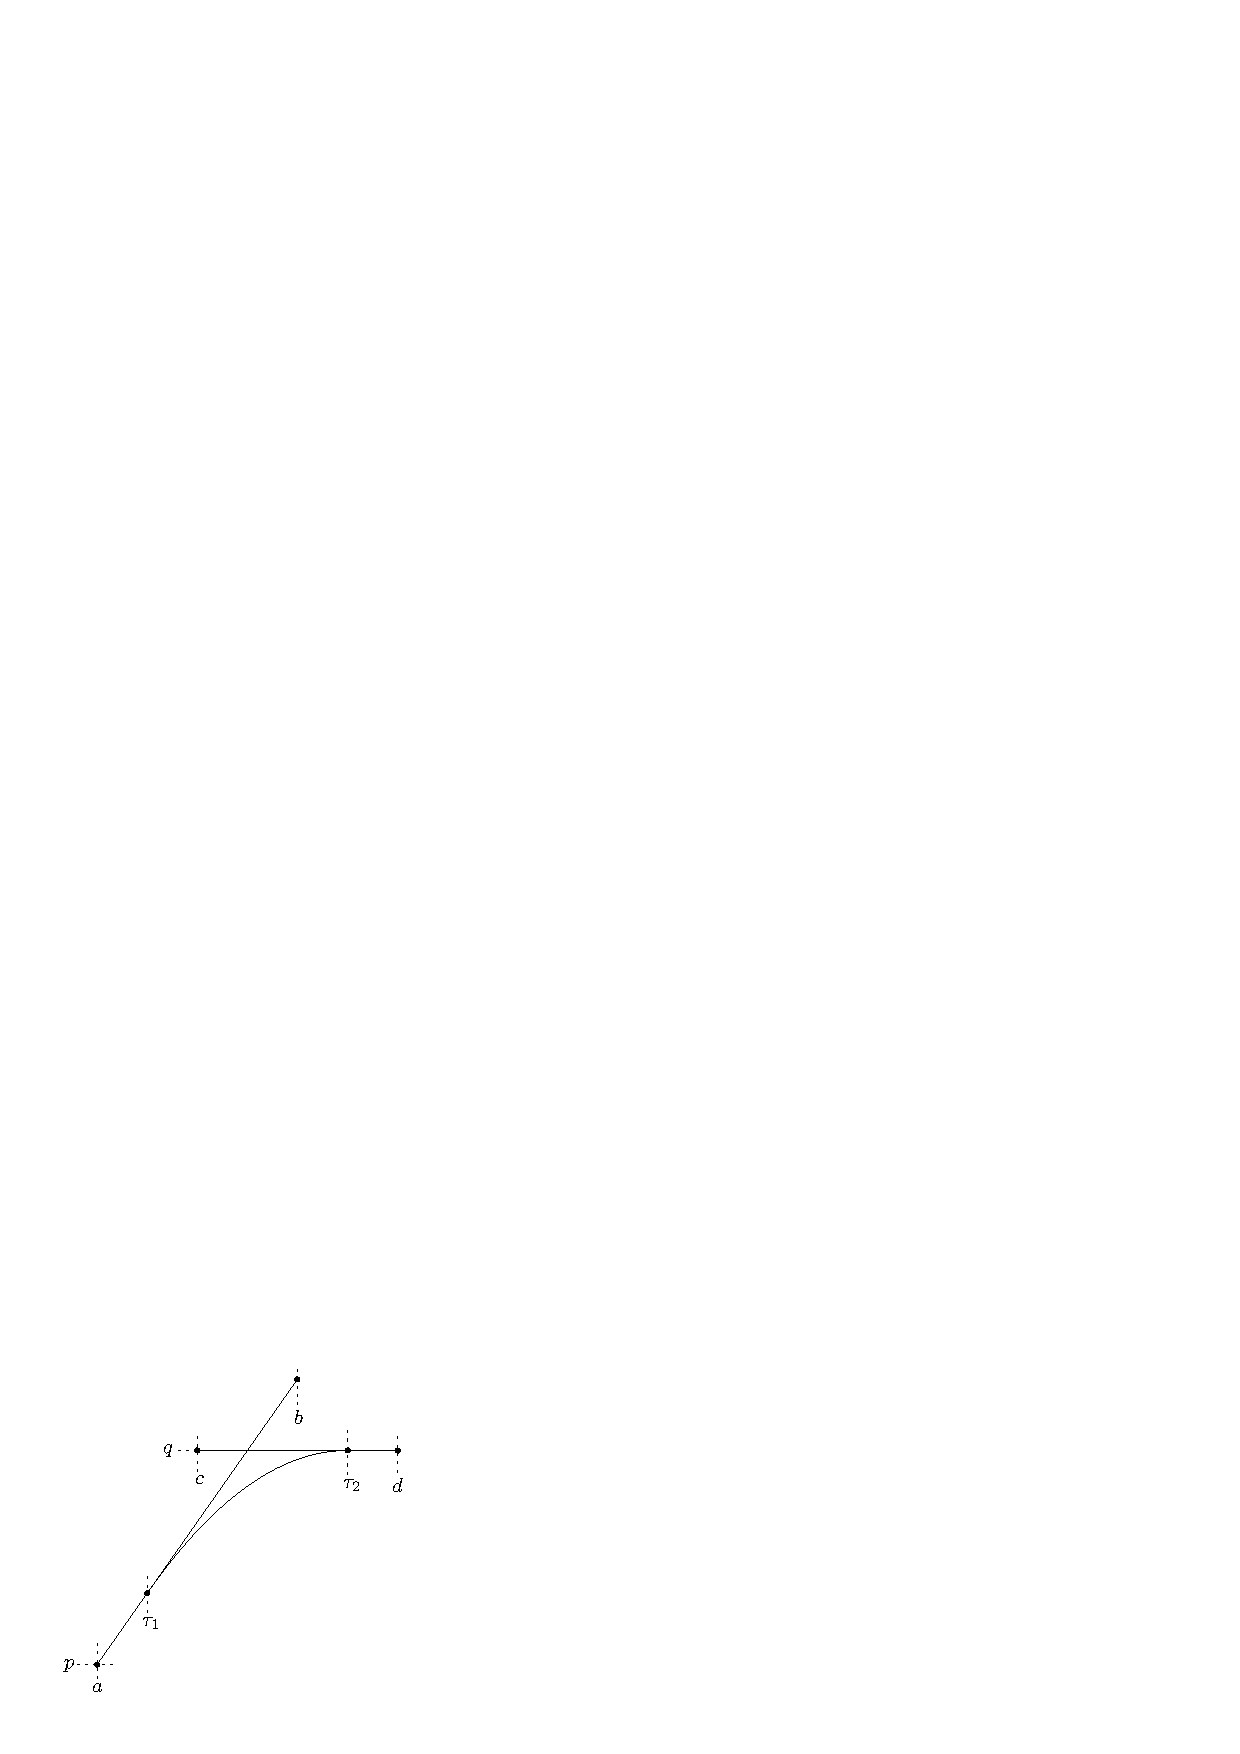
\includegraphics[width=0.9\linewidth]{figures/motion/lemma_full_still}
  \captionof{figure}{$x^{1} \rightarrow x^{0}$}
  \label{fig:full_still}
\end{minipage}%
\hspace{1.0em}
\begin{minipage}{.45\textwidth}
  \centering
  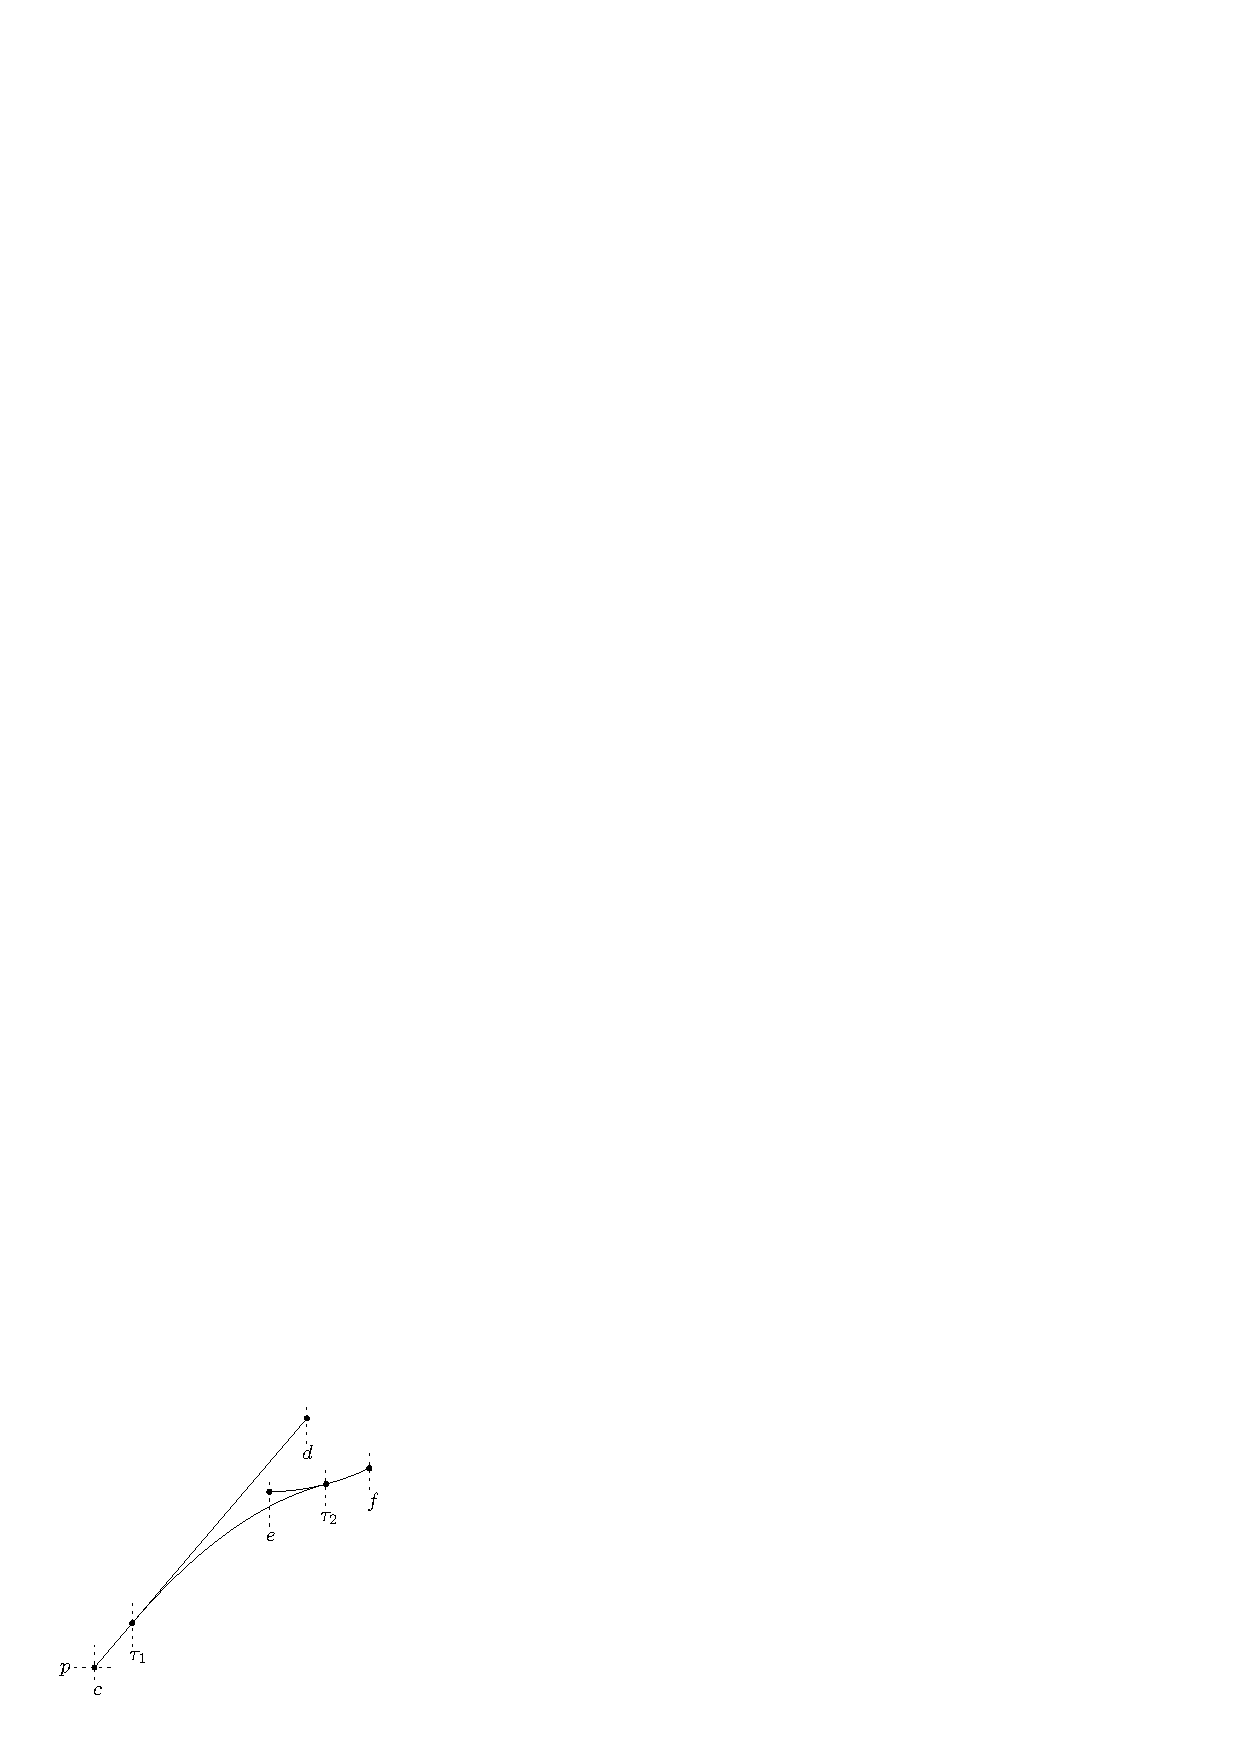
\includegraphics[width=0.9\linewidth]{figures/motion/lemma_full_acc}
  \captionof{figure}{$x^{1} \rightarrow x^{+}$}
  \label{fig:full_acc}
\end{minipage}
\end{figure}


  % {\color{Navy}
  % Expanding the left-hand side of the state equation gives
  % \begin{align*}
  %   x^{-}[x^{1}[p,a,b](\tau_{1}), \tau_{1}, \tau_{2}](\tau_{2}) =
  %   \begin{pmatrix}
  %     p + \tau_{1} - a + (\tau_{2} - \tau_{1}) - \omega(\tau_{2} - \tau_{1})^{2}/2 \\
  %     1 - \omega(\tau_{2} - \tau_{1})
  %   \end{pmatrix} .
  % \end{align*}
  % }

% \begin{lemma}[$x^{1} \rightarrow x^{+}$]
%   Let $x^{1}[p, a, b]$ and $x^{+}[x, c, d]$ be two trajectories.
%   Considering $\tau_{1}$ and $\tau_{2}$ as variables in the equation
%   \begin{align*}
%     x^{-}[x^{1}[p,a,b](\tau_{1}), \tau_{1}, \tau_{2}](\tau_{2}) = x^{+}[x, c, d](\tau_{2}),
%   \end{align*}
%   it has solution $\dots$.
% \end{lemma}
% \begin{proof}
%   Expanding the state equation gives the system of equations
%   \begin{align*}
%     \begin{cases}
%       p - a + \tau_{2} - \omega (\tau_{2} - \tau_{1})^{2}/2 = x_{1} + x_{2}(\tau_{2} - c) + \omega(\tau_{2} - c)^{2} / 2 \\
%       1 - \omega(\tau_{2} - \tau_{1}) = x_{2} + \omega(\tau_{2} - c)
%     \end{cases}
%   \end{align*}
%   We use the second equation to derive
%   $\tau_{2} - \tau_{1} = (1-x_{2})/\omega - \tau_{2} + c$. Substituting this in
%   the first equation yields the quadratic equation
%   \begin{align*}
%     \omega (\tau_{2} - c)^{2} - 2(1-x_{2})\tau_{2} - 2cx_{2} - p + a + c + x_{1} + (1-x_{2})^{2}/2\omega = 0
%   \end{align*}
% \end{proof}

To keep the expressions for the case of joining $x^{1} \rightarrow x^{+}$ a
little bit simpler, we first consider a full line joining to a acceleration
trajectory of full length $1/\omega$.

\begin{lemma}
  \label{lemma:line_acc}
  Consider some full acceleration trajectory $x^{+}[(p, 0), a, a+1/\omega]$ and the
  line through $(\lambda, 0)$ with slope 1. Whenever $\lambda$, which can be
  interpreted as a time epoch, satisfies $\lambda \in [a-p-1/2\omega, a-p+1/2\omega]$, then the equation
  \begin{align*}
    x^{+}[(p, 0), a, a+1/\omega](\tau) = x^{-}[(q, 1), q + \lambda, q + \lambda + 1/\omega](\tau) ,
  \end{align*}
  with $\tau$ and $q$ considered as variables, has a unique solution
  \begin{align*}
    \tau &= a + 1/\omega - \sqrt{\frac{a - p + 1/2\omega - \lambda}{\omega}} , \\
    q &= 2\tau - a - 1/\omega - \lambda ,
  \end{align*}
  so the joining deceleration is given by $x^{-}[(q,1), q + \lambda, \tau]$
\end{lemma}
\begin{proof}
  First of all, the expanded system of state equations is given by
  \begin{align*}
    \begin{cases}
    p + \omega (\tau - a)^{2}/2 = q + (\tau - q - \lambda) - \omega (\tau - q - \lambda)^{2}/2 , \\
    \omega(\tau - a) = 1 - \omega(\tau - q - \lambda) .
      \end{cases}
  \end{align*}
  We use the second equation to express $q$ in terms of $\tau$, which yields
  \begin{align*}
    q = 2\tau - 1/\omega -a - \lambda ,
  \end{align*}
  which we substitute in the first equation to derive the equation
  \begin{align*}
    \omega \tau^{2}  - 2 (1 + \omega a) \tau + \omega a^{2} + a + p + \lambda + 1/2\omega = 0 .
  \end{align*}
  This is a quadratic equation in $\tau$, with solutions
  \begin{align*}
    \tau = a + 1/\omega \pm \sqrt{\frac{a - p + 1/2\omega - \lambda}{\omega}} ,
  \end{align*}
  of which only the smallest one is valid, because $\tau \leq a + 1/\omega$.
  Furthermore, we see that $\tau$ is defined as a real number when
  \begin{align*}
    a - p + 1/2\omega - \lambda \geq 0 \iff \lambda \leq a - p + 1/2\omega .
  \end{align*}
  The other requirement is that $\tau \geq a$, which is equivalent to
  \begin{align*}
    1/\omega \geq \sqrt{\frac{a - p + 1/2\omega - \lambda}{\omega}} \iff
    % 1/\omega \geq a - p - \lambda + 1/2\omega \iff
    \lambda \geq a - p - 1/2\omega .
  \end{align*}
\end{proof}

\begin{lemma}[$x^{1} \rightarrow x^{+}$]
Consider partial trajectories $x^{1}[p, c, d]$ and $x^{+}[x, e, f]$.
\end{lemma}
\begin{proof}
  First of all, observe that $x^{1}[p, c, d]$ lies on the line with slope 1
  through $(\lambda, 0) := (c - p, 0)$ and $x^{+}[x, e, f]$ lies on the full
  acceleration curve
  $x^{+}[(x_{1} - x_{2}^{2}/(2\omega) , 0), e - x_{2}/\omega, e - x_{2}/\omega + 1/\omega]$, see
  Figure~\ref{fig:full_acc}.
  %
  Now apply Lemma~\ref{lemma:line_acc} to $p = x_{1} - x_{2}^{2}/(2\omega)$,
  $a = e - x_{2}/\omega$ and $\lambda = c - p$ yields some solutions $\tau$ and $q$.
  %
  Let $\tau_{2} := \tau$ and let $\tau_{1}$ denote the time where the line and
  $x^{+}$ join, given by $\tau_{1} = \lambda + q$. Now we simply check whether this
  solution is also feasible for the smaller trajectories. We must have
  $\tau_{1} \in [c, d]$ and $\tau_{2} \in [e, f]$.
\end{proof}


\begin{lemma}
  \label{lemma:acc_hline}
  Consider the acceleration trajectory $x^{+}[(p, 0), a, b]$ and the horizontal
  line through $(0, q)$. Let $\tau_{1} = a + \sqrt{(q-p)/\omega}$ and
  $\tau_{2} = a + 2\sqrt{(q-p)/\omega}$. If $\tau_{1}$ satisfies
  $\tau_{1} \in [a, b]$, then both trajectories are joined by deceleration
  trajectory $x^{-}[x^{+}[(p, 0), a, b](\tau_{1}), \tau_{1}, \tau_{2}]$
\end{lemma}
\begin{proof}
  Consider the following equation
  \begin{align*}
    x^{-}[x^{+}[(p, 0),a,b](\tau_{1}), \tau_{1}, \tau_{2}](\tau_{2}) = (q, 0) .
  \end{align*}
  %
  The expanded system of state equations is given by
  \begin{align*}
    \begin{cases}
      p + \omega (\tau_{1} - a)^{2}/2 + (\omega(\tau_{1} - a)) (\tau_{2} - \tau_{1}) - \omega(\tau_{2} - \tau_{1})^{2}/2 = q , \\
      \omega(\tau_{1} - a) - \omega(\tau_{2} - \tau_{1}) = 0 .
    \end{cases}
  \end{align*}
  From the second equation, we derive $\tau_{1} - a = \tau_{2} - \tau_{1}$.
  Plugging this back in the first equation yields the quadratic equation
  $p + \omega(\tau_{1} - a)^{2} = q$ with solutions
  $\tau_{1} = a \pm \sqrt{(q-p)/\omega}$, of which only the larger one is valid.
  Finally, the second equation gives $\tau_{2} = 2\tau_{1} - a$.
\end{proof}

\begin{lemma}[$x^{+} \rightarrow x^{0}$]
  Consider partial trajectories $x^{+}[x, c, d]$ and $x^{0}[q, e, f]$.
\end{lemma}
\begin{proof}
  Observe that $x^{+}[x, c, d]$ lies on the full acceleration curve
  $x^{+}[(x_{1} - x_{2}^{2}/(2\omega), 0), c - x_{2}/\omega, c - x_{2}/\omega + 1/\omega]$.
  Hence, we can apply Lemma~\ref{lemma:acc_hline} with
  $p=x_{1} - x_{2}^{2}/(2 \omega)$, $a = c - x_{2}/\omega$, which yields some
  solutions $\tau_{1}$ and $\tau_{2}$, which are feasible solutions if
  $\tau_{1} \in [c, d]$ and $\tau_{2} \in [e, f]$.
\end{proof}

\begin{lemma}
  Consider full acceleration trajectories $x^{+}[(p, 0), a, b]$ and
  $x^{+}[(q, 0), c, d]$.
\end{lemma}
\begin{proof}
  Consider the equation
  \begin{align*}
    x^{-}[x^{+}[(p, 0), a, b](\tau_{1}), \tau_{1}, \tau_{2}](\tau_{2}) = x^{+}[(q, 0), c, d](\tau_{2}) ,
  \end{align*}
  expanded to the system of equations
  \begin{align*}
    \begin{cases}
      p + \omega(\tau_{1} - a)^{2}/2 + \omega(\tau_{1} - a)(\tau_{2} - \tau_{1}) - \omega(\tau_{2} - \tau_{1})^{2}/2 = q + \omega(\tau_{2} - c)^{2}/2 , \\
      \omega(\tau_{1} - a) + \omega(\tau_{2} - \tau_{1}) = \omega(\tau_{2} - c) .
    \end{cases}
  \end{align*}
\end{proof}

\begin{lemma}[$x^{+} \rightarrow x^{+}$]
  Consider partial trajectories $x^{+}[x, a, b]$ and $x^{+}[y, c, d]$.
\end{lemma}
\begin{proof}

\end{proof}

\newpage

Let $D[t_{0}, t_{1}]$ denote the set of all state trajectories
$x : [t_{0}, t_{1}] \rightarrow \mathbb{R}^{2}$ satisfying the double integrator
dynamics $\dot{x}_{1} = x_{2}, \dot{x}_{2} = u$, the speed constraint
$x_{2} \in [0, 1]$ and control constraint $u \in [-\omega, \omega]$.
Let $\bar{D}[t_{0}, t_{1}] \subset D[t_{0}, t_{1}]$ denote the set of
trajectories $x$ satisfying $x(t_{1}) = (0, 1)$. Let
$\widetilde{D}[t_{0}, t_{1}] \subset \bar{D}[t_{0}, t_{1}]$ denote those that
further satisfy $x(t_{0}) = (p_{0}, 1)$.
%
Furthermore, for each of the previous three sets, we use the notation
$D_{1}[t_{0}, t_{1}]$ to refer to the set of corresponding trajectories of the
position component $x_{1}$ only.

\begin{lemma}
  \label{lemma:above}
  Let $g, h \in D_{1}[a, b]$ such that $h''(t) = -\omega$ for all $t$. If
  $g(a) \geq h(a)$ and $g'(a) > h'(a)$, then $g(t) > h(t)$ for
  $t \in \openhalf{a}{b}$.
\end{lemma}
\begin{proof}
  For any $t \in [a, b]$, we have
  $g'(t) \geq g'(a) - \omega (t-a) > h'(a) - \omega(t-a) = h'(t)$.
\end{proof}

\begin{lemma}
  \label{lemma:below}
  Let $g, h \in D_{1}[a, b]$ such that $h''(t) = \omega$ for all $t$. If
  $g(a) \leq h(a)$ and $g'(a) < h'(a)$, then $g(t) < h(t)$ for
  $t \in \openhalf{a}{b}$.
\end{lemma}
\begin{proof}
  For any $t \in [a, b]$, we have
  $g'(t) \leq g'(a) + \omega (t-a) < h'(a) + \omega(t-a) = h'(t)$.
\end{proof}

\begin{lemma}
  \label{lemma:cross-dec}
  Consider $g,h \in D_{1}[a, b]$ such that $h''(t) = -\omega$ for all $t$.
  Suppose there is some touching time $c \in \openhalf{a}{b}$ such that $g(c) = h(c)$, then
  we have
  \begin{align*}
    g(a) < h(a) \implies g'(c) > h'(c) .
  \end{align*}
\end{lemma}
\begin{proof}
  Let $g(a) < h(a)$ and consider the smallest time $c \in \openhalf{a}{b}$ such
  that $g(c) = h(c)$. Suppose that $g'(c) = h'(c)$. Let $f:= h - g$, so we have
  $f(t) > 0$ for $t \in \halfopen{a}{c}$. Using the Taylor expansion of $f$
  around $c$ with $\tau > 0$, we derive
  \begin{align*}
    0 < f(c - \tau) &= f(c) - f'(c)\tau + f''(c)\tau^{2} / 2 + o(\tau^{2}) \\
    % &= h(c) - g(c) + (h'(c) - g'(c))\tau + (h''(c) - g''(c))\tau^{2} / 2 + o(\tau^{2}) \\
    &= (h''(c) - g''(c))\tau^{2} / 2 + o(\tau^{2}) \\
    &= (-\omega - g''(c))\tau^{2} / 2 + o(\tau^{2}) .
  \end{align*}
  Now dividing by $\tau^{2}$ and taking the limit $\tau \downarrow 0$ gives
  $g''(c) < -\omega$, which contradicts $g \in D_{1}[a,b]$. Hence, we have
  $g'(c) \neq h'(c)$. Observe that $g'(c) < h'(c)$ would mean that
  $g(c - \epsilon) \geq h(c - \epsilon)$ for some $\epsilon > 0$, contradicting our assumption that $c$
  was smallest. Therefore, we have shown that $g'(c) > h'(c)$. Hence, it follows
  from Lemma~\ref{lemma:above} that there can only be a single touching time $c$, which completes
  the proof.
\end{proof}

\begin{lemma}
  \label{lemma:cross-acc}
  Consider $g,h \in D_{1}[a, b]$ such that $h''(t) = \omega$ for all $t$.
  Suppose there is some touching time $c \in \openhalf{a}{b}$ such that $g(c) = h(c)$, then
  we have
  \begin{align*}
    g(a) > h(a) \implies g'(c) < h'(c) .
  \end{align*}
\end{lemma}
\begin{proof}
  Let $g(a) > h(a)$ and consider the smallest time $c \in \openhalf{a}{b}$ such
  that $g(c) = h(c)$. Suppose that $g'(c) = h'(c)$. Let $f:= h - g$, so we have
  $f(t) < 0$ for $t \in \halfopen{a}{c}$. Using the Taylor expansion of $f$
  around $c$ with $\tau > 0$, we derive
  \begin{align*}
    0 > f(c - \tau) &= f(c) - f'(c)\tau + f''(c)\tau^{2} / 2 + o(\tau^{2}) \\
    % &= h(c) - g(c) + (h'(c) - g'(c))\tau + (h''(c) - g''(c))\tau^{2} / 2 + o(\tau^{2}) \\
    &= (h''(c) - g''(c))\tau^{2} / 2 + o(\tau^{2}) \\
    &= (\omega - g''(c))\tau^{2} / 2 + o(\tau^{2}) .
  \end{align*}
  Now dividing by $\tau^{2}$ and taking the limit $\tau \downarrow 0$ gives
  $g''(c) > \omega$, which contradicts $g \in D_{1}[a,b]$. Hence, we have
  $g'(c) \neq h'(c)$. Observe that $g'(c) > h'(c)$ would mean that
  $g(c - \epsilon) \leq h(c - \epsilon)$ for some $\epsilon > 0$, contradicting our assumption that $c$
  was smallest. Therefore, we have shown that $g'(c) < h'(c)$. Hence, it follows
  from Lemma~\ref{lemma:below} that there can only be a single touching time $c$, which completes
  the proof.
\end{proof}


We first analyze the special case when the crossing time of the lead boundary
coincides with the scheduled crossing time of the current vehicle.

\begin{lemma}[Entry]
  \label{lemma:entry}
  Let $\bar{x} \in \bar{D}[t_{0}, t_{1}]$ be some lead boundary with control
  function $\bar{u}$ with alternating intervals
  $\bar{F}_{i}, \bar{D}_{i}, \bar{S}_{i}, \bar{A}_{i}$. Assume that problem
  \begin{align*}
    x^{*} := \arg\max_{x} \; &\int_{t_{0}}^{t_{1}} x_{1}(t) dt \\
            &x \in \widetilde{D}[t_{0}, t_{1}] , \\
            &x_{1}(t) \leq \bar{x}_{1}(t)  \text{ for all } t \in [t_{0}, t_{1}] ,
  \end{align*}
  is feasible, then an optimal trajectory $x^{*}$ is determined by the control
  ($t_{d1}$ and $\tau_{1}$ in proof)
  \begin{align*}
    u(t) = \begin{cases}
             0     &\text{ for } t \in (0, t_{d1}) , \\
             -\omega    &\text{ for } t \in (t_{d1}, \tau_{1}) , \\
             \bar{u}(t) &\text{ for } t \in (\tau_{1}, t_{1}) .
            \end{cases}
  \end{align*}

\end{lemma}
\begin{proof}
  \phantom{.}
  \begin{itemize}
    \item Assume feasibility (which means that $\underline{x}$ exists, analyze the exact
          conditions somewhere separately). Hence $t_{0} \leq t_{1} + p_{0}$
          (otherwise $\bar{x}(t_{1})$ would not be reachable). The case
          $t_{0} = t_{1} + p_{0}$ is trivial, because the optimal trajectory is
          to simply continue at full speed. When $t_{0} < t_{1} + p_{0}$, we
          need at least one interval of deceleration.
    \item Let $\tau_{1}$ denote the earliest possible entry time, which is the smallest
          time $t$ such that $x(t) = \bar{x}(t)$. This time is obviously
          well-defined, because $x(t_{1}) = \bar{x}(t_{1})$ by assumption. Next,
          we do a case distinction on where $\tau_{1}$ is on the lead vehicle
          boundary in terms of the type of alternating interval. For each case,
          we construct a feasible trajectory $x^{*}$ with one deceleration of
          length $d$ until $\tau_{1}$.
    \item Suppose $\tau_{1} \in \bar{S}_{i}$ for some $i$, then
          $x_{2}^{*}(\tau_{1}) = \bar{x}_{2}(\tau_{1}) = 0$. This implies that
          $u^{*}(t) = -\omega$ for $t \in (\tau_{1} - 1/\omega, \tau_{1})$ and
          $u^{*}(t) = 0$ for $t \in (t_{0}, \tau_{1} - 1/\omega)$. Hence, the
          position at the entry time needs to satisfy
          \begin{align*}
            \bar{x}_{1}(\bar{t}_{si}) = x^{*}_{1}(\tau_{1}) &= p_{0} + \tau_{1} - 1/\omega - t_{0} + p^{-}(1/\omega) \\
                                &= p_{0} + \tau_{1}- t_{0} -1/2\omega ,
          \end{align*}
          from which we derive that
          \begin{align*}
            \tau_{1} = t_{0} - p_{0} + 1/2\omega + \bar{x}_{1}(\bar{t}_{si}) .
          \end{align*}
          Furthermore, we have $t_{d1} = \tau_{1} - 1/\omega$.

    \item Suppose $\tau_{1} \in \bar{A}_{i}$ for some $i$, then
          $x_{1}^{*}(\tau_{1}) = \bar{x}_{1}(\tau_{1}) = \bar{x}_{1}(\bar{t}_{ai}) + p^{+}(\tau_{1} - \bar{t}_{ai}; \bar{x}_{2}(\bar{t}_{ai})) $
          and
          $x_{2}^{*}(\tau_{1}) = \bar{x}_{2}(\tau_{1}) = \bar{x}_{2}(\bar{t}_{ai}) + (\tau_{1} - \bar{t}_{ai}) \omega$.
          This means that the duration of the initial deceleration $d$ must be
          given by
          \begin{align*}
            d = \frac{1 - x^{*}_{2}(\tau_{1})}{\omega} = \frac{1 - \bar{x}_{2}(\bar{t}_{ai})}{\omega} - \tau_{1} + \bar{t}_{ai} .
          \end{align*}
          Observe that, starting from the initial position, the current vehicle
          drives at full speed for a duration of $\tau_{1} - d - t_{0}$ before
          decelerating, so the position of the entry point is given by
          \begin{align*}
            x^{*}_{1}(\tau_{1}) &= p_{0} + \tau_{1} - d - t_{0} + p^{-}(d) , \\
                    &= p_{0} + \tau_{1} - t_{0} - \omega d^{2} / 2 .
          \end{align*}
          %
          We can find $\tau_{1}$ by equating $x^{*}_{1}(\tau_{1}) = \bar{x}_{1}(\tau_{1})$,
          which yields the quadratic equation
          \begin{align*}
            &p_{0} + \tau_{1} - t_{0} - \omega d^{2} / 2 = \bar{x}_{1}(\bar{t}_{ai}) + \bar{x}_{2}(\bar{t}_{ai})(\tau_{1} - \bar{t}_{ai}) + \omega (\tau_{1} - \bar{t}_{ai})^{2} / 2 , \\
            &\begin{aligned}
            \; \implies \tau_{1} &= \bar{t}_{ai} -\frac{\bar{x}_{2}(\bar{t}_{ai})}{\omega} + \frac{1}{\omega} \\
            &\quad- \frac{1}{2}\sqrt{\frac{2}{\omega^{2}} + \frac{2(\bar{x}_{2}(\bar{t}_{ai}))^{2}}{\omega^{2}} + 4\left( \frac{p_{0} - t_{0} - \bar{x}_{1}(\bar{t}_{ai}) + \bar{t}_{ai}(1 + \bar{x}_{2}(\bar{t}_{ai}))}{\omega} \right)} \\
            t_{d1} &= \tau_{1} - d = 2 \tau_{1} - \bar{t}_{ai} + \frac{\bar{x}_{2}(\bar{t}_{ai}) - 1}{\omega} .
            \end{aligned}
          \end{align*}


    \item If $\tau_{1} \in \bar{F}_{i} \cup \bar{D}_{i}$, then we show that
          $\tau_{1} = t_{fi}$, so this case reduces to
          $\tau_{1} \in \bar{A}_{i}$.
          %
          Suppose there exists a trajectory $x \in \widetilde{D}[t_{0}, t_{1}]$
          and let $\tau_{1}$ denote its earliest entry time. First of all, if
          $\tau_{1} \in \bar{F}_{i}$ for some $i$, then it is obvious that
          $\tau_{1} = \bar{t}_{fi}$. Next, suppose
          $\tau_{1} \in \openhalf{\bar{t}_{di}}{\bar{t}_{si}}$, so
          $x_{1}(\bar{t}_{di}) < \bar{x}_{1}(\bar{t}_{di})$, then applying
          Lemma~\ref{lemma:cross-dec} yields $x_{2}(\tau_{1}) > \bar{x}_{2}(\tau_{1})$,
          contradicting the fact that $\tau_{1}$ was an entry time.

    \item Show that $x^{*}_{1}$ is an upperbound for any $x_{1} \in \widetilde{D}_{1}[t_{0},t_{1}]$.
          %
          Let $\tau_{0}^{*}$ denote the start of the first deceleration of
          $x^{*}$. Let $x$ be some feasible solution, then
          $x_{1}(t) \leq \bar{x}_{1}(t) = x_{1}^{*}(t)$ for
          $t \in [\tau_{1}, t_{1}]$. We show that $x_{1}(t) \leq x^{*}_{1}(t)$
          on $t \in [t_{0}, \tau_{1}]$ as well. Let $\tau_{0}$ denote the start
          of the first deceleration of $x$.
          %
          Suppose $\tau_{0} > \tau_{0}^{*}$, then we have
          $x_{1}(\tau_{0}) > x^{*}_{1}(\tau_{0})$ and
          $x_{2}(\tau_{0}) = 1 > x_{2}^{*}(\tau_{0}) = 1 - \omega (\tau_{0} - \tau_{0}^{*})$,
          so by applying Lemma~\ref{lemma:above} for $x^{*}$ and $x$ on
          $[\tau_{0}, \tau_{1}]$, we have
          $x_{1}(\tau_{1}) > x^{*}_{1}(\tau_{1}) = \bar{x}_{1}(\tau_{1})$, which
          violates the feasibility of $x$.
          %
          Suppose $\tau_{0} < \tau_{0}^{*}$, then we obviously must have
          $x_{1}(\tau_{0}^{*}) < x_{1}^{*}(\tau_{0}^{*})$. Suppose that
          $c = \inf\{ t \in (\tau_{0}^{*}, \tau_{1}): x_{1}(t) > x_{1}^{*}(t) \}$
          exists, i.e., $x$ crosses $x^{*}$ at $c$ for the first time.
          Application of Lemma~\ref{lemma:cross-dec} gives
          $x_{2}(c) > x^{*}_{2}(c)$. But then it follows from
          Lemma~\ref{lemma:above} that
          $x_{1}(\tau_{1}) > x_{1}^{*}(\tau_{1}) = \bar{x}_{1}(\tau_{1})$, which
          violates the feasibility of $x$.

    \item Now $x^{*}$ is optimal, because
          $\int_{t_{0}}^{t_{1}} x_{1}^{*}(t) dt \geq \int_{t_{0}}^{t_{1}} x_{1}(t) dt$
          for any $x \in \widetilde{D}_{1}[t_{0},t_{1}]$. \qedhere
  \end{itemize}
\end{proof}

We now consider the general case in which the scheduled crossing time does not
need to coincide with the end of the lead vehicle boundary.
%
Invoke Lemma~\ref{lemma:entry} to obtain $\bar{x}'$ and argue that it is a valid
upperbound for any feasible trajectory, so we can use it instead of $\bar{x}$
without changing the problem.

\begin{lemma}[Exit]
  \label{lemma:exit}
  Let $\bar{x}' \in \widetilde{D}[t_{0}, t_{1}]$ be some lead boundary. Let $t_{2} > t_{1}$, and assume that problem
  \begin{align*}
    x^{*} = \arg\max_{x} \; &\int_{t_{0}}^{t_{1}} x_{1}(t) dt \\
            &x \in \widetilde{D}[t_{0}, t_{2}] , \\
            &x_{1}(t) \leq \bar{x}'_{1}(t)  \text{ for all } t \in [t_{0}, t_{1}] ,
  \end{align*}
  is feasible, then an optimal trajectory $x^{*}$ is given by \dots
\end{lemma}
\begin{proof}
  \phantom{.}
  \begin{itemize}
    \item We define the boundary $\bar{x}''$ by $\bar{x}''(t) = 1/2\omega$ for
          $t \leq t_{1} - 1/\omega$ and
          $\bar{x}''(t) = x^{+}[(-1/2\omega, 0), t_{1} - 1/\omega, t_{1}](t)$
          for $t \in [t_{1} - 1/\omega, t_{1}]$. We argue that $\bar{x}''$ is an
          upperbound for all feasible trajectories. Let
          $x \in \widetilde{D}[t_{0}, t_{2}]$ be any trajectory that has
          $x_{1}(t) > -1/2\omega$ for some $t \leq t_{0} - 1/\omega$, so that
          $x_{1}(t_{0} - 1/\omega) > -1/2\omega = \bar{x}_{1}''(t_{0} - 1/\omega)$.
          Now because $x \in \widetilde{D}[t_{0}, t_{1}]$, we have
          $x(t_{2}) = \bar{x}''(t_{2}) = (0, 1)$, but
          Lemma~\ref{lemma:cross-acc} yields
          $x_{2}(t_{2}) < \bar{x}''(t_{2}) = 1$, a contradiction.

    \item Next, we construct a trajectory $x^{*}$ by joining $\bar{x}'$ and
          $\bar{x}''$ using a deceleration part $x^{-}$. Argue that such $x^{*}$
          must always exist. Argue that $x^{*}$ is unique.

    \item We argue that $x^{*}$ is an upperbound for any feasible trajectory.
          First of all, $\bar{x}'$ is an upperbound, so
          $x_{1}(\tau_{1}) \leq \bar{x}_{1}'(\tau_{1})$. Suppose there is some
          $c \in (\tau_{1}, \tau_{2})$ such that $x$ crosses $x^{-}$, so
          $x_{1}(c) = x_{1}^{-}(c)$ and $x_{2}(c) > x_{2}^{-}(c)$, then by
          Lemma~\ref{lemma:above}, we have
          $x_{1}(\tau_{2}) > x^{-}_{1}(\tau_{2}) = \bar{x}_{1}''(\tau_{2})$,
          which contradicts the fact that $\bar{x}''$ is an upperbound.

    \item Now $x^{*}$ is optimal, because
          $\int_{t_{0}}^{t_{2}} x_{1}^{*}(t)dt \geq \int_{t_{0}}^{t_{2}} x_{1}(t) dt$
          for any $x \in \widetilde{D}_{1}[t_{0}, t_{2}]$.


    % \item Let $\tau_{2}$ denote the latest possible exit time, which is the smallest
    %       $t$ such that there exists a feasible $x$ with $x(t) = \bar{x}(t)$.
    %       This time is well-defined, because $x(t_{0}) = \bar{x}(t_{0})$ by
    %       assumption. Next, we do a case distinction on where $\tau_{2}$ is on the
    %       bounary in terms of the type of alternating interval. For each case,
    %       we construct a feasible trajectory $x^{*}$ with one deceleration and
    %       one acceleration.
  \end{itemize}
\end{proof}


\newpage
\section{Platoons in tandem of two intersections}

\begin{figure}
  \centering
  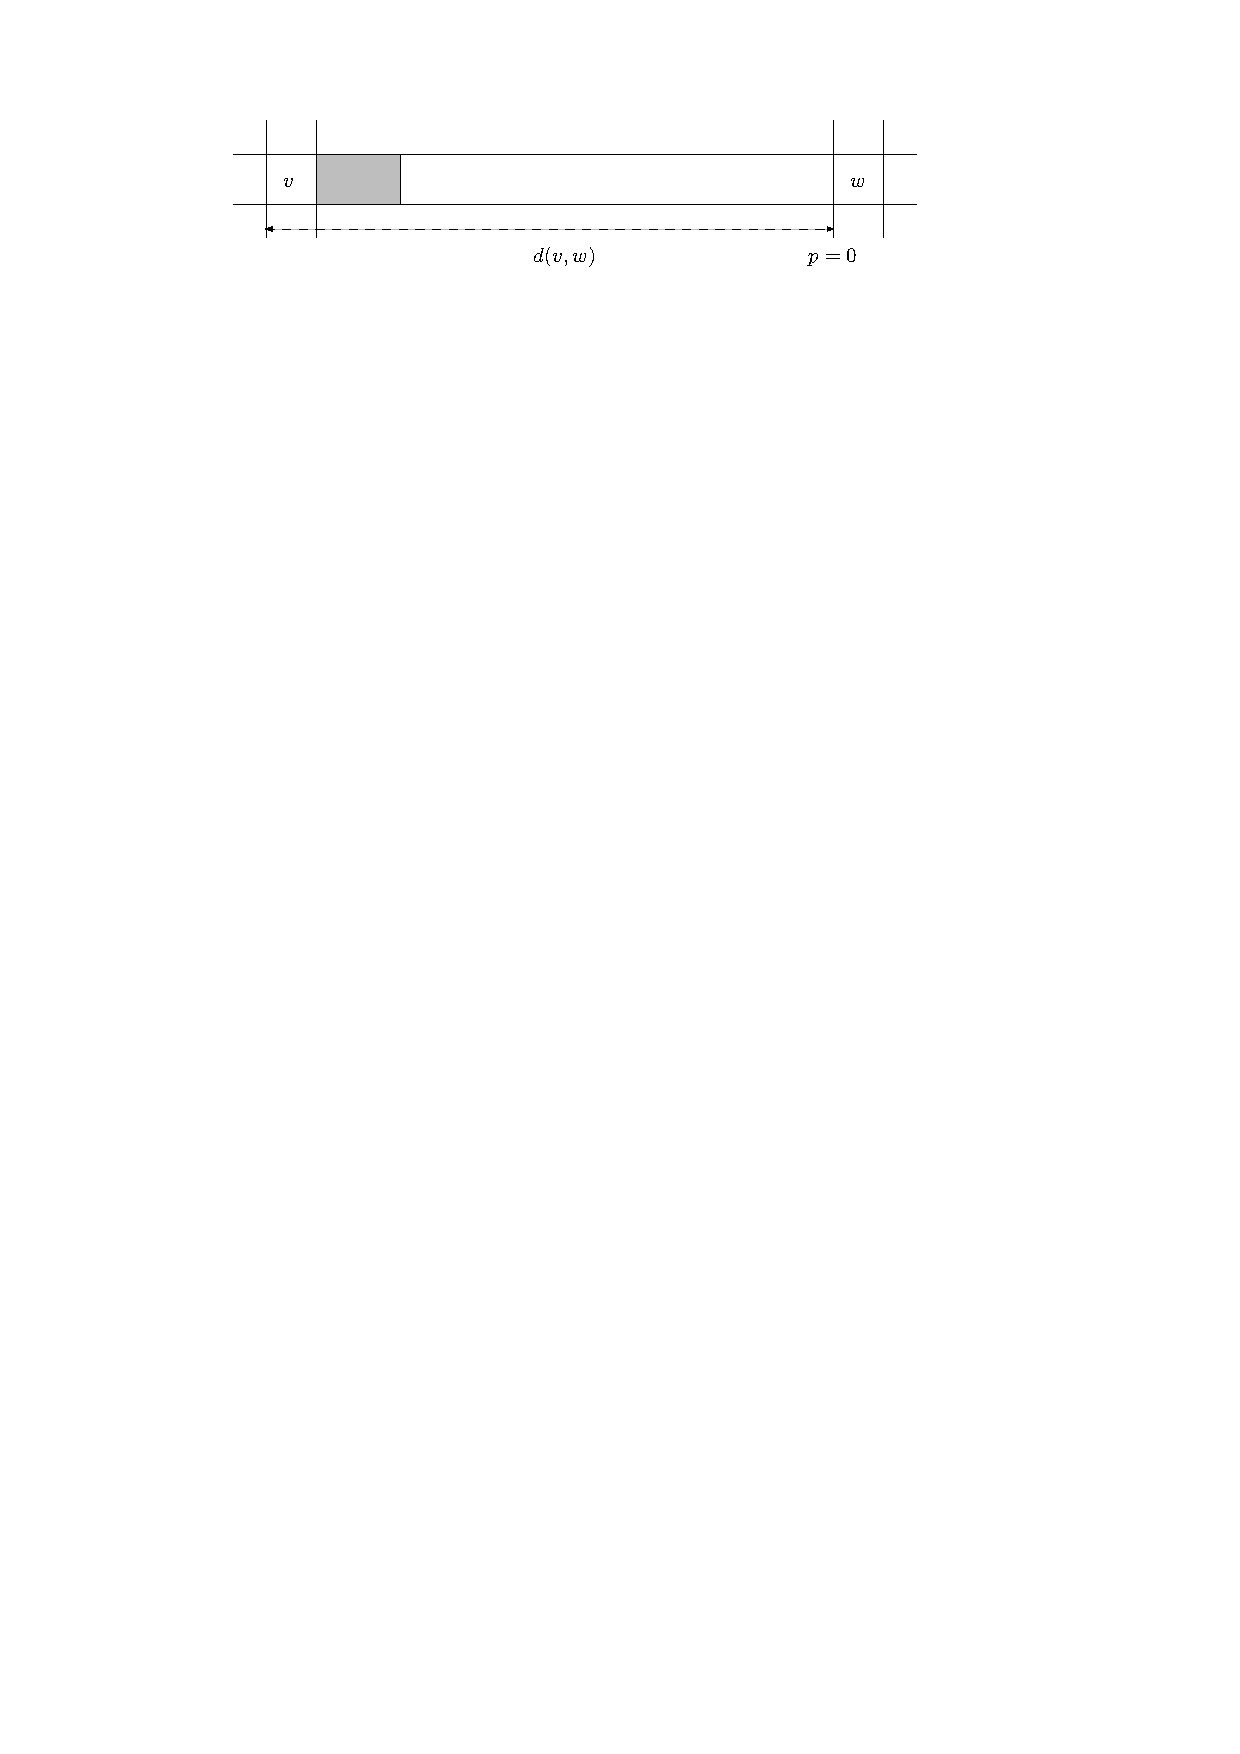
\includegraphics[width=0.99\textwidth]{figures/motion/tandem}
  \caption{Tandem of two intersections $v$ and $w$ with lane of length $d(v,w)$.
    The grey rectangle represents some vehicle that just left intersection $v$.
    We assume that vehicles must drive at maximum speed as long as they occupy
    any intersection, so deceleration is only allowed from the shown position
    onwards.}
  \label{fig:tandem}
\end{figure}

When considering multiple vehicles driving between intersection, we must take
into account the capacity of the lane segment between them, because the fact
that only a limited number of vehicles can drive or wait at the same time on a
lane between intersections may cause network-wide effects.
%
The capacity of lanes between intersections is intimately related to the
trajectories of vehicles, which we first want to understand better. We will be
using an optimal control formulation with the objective that keeps the vehicles
as close as possible to the next intersection at all times, which is similar to
the MotionSynthesize problem considered in
\cite{miculescuPollingsystemsbasedAutonomousVehicle2016}. This problem can be
solved using direct transcription, which works well enough if we just want to
simulate the behavior of the system. However, we show that it is possible to
explicitly formulate the optimal controller and explain how to compute
trajectories without using time discretization.

\subsection{Problem formulation}

Before we turn to the general case of networks of intersection, we will first
investigate the trajectories of vehicles in a tandem of two intersections as
depicted in Figure~\ref{fig:tandem}. Let $v$ denote the left intersection and
$w$ the right intersection and assume that vehicles drive from left to right.
% We will sometimes refer to intersection $w$ as the downstream intersection.
Furthermore, we will call the road segment strictly between both intersection
areas the \textit{lane}. In the following discussion, let $p(t)$ and $v(t)$ denote the
position and velocity of the vehicle, respectively, and we call
$x(t) = (p(t), v(t))$ its \textit{state}. Let the length and width of a vehicle
$i$ be denoted by $L_{i}$ and $W_{i}$, respectively. We measure the position of
a vehicle at the front bumper. We fix position $p=0$ at the stop line of
intersection $w$.
%
We make the following additional assumptions about our lane model.

\begin{assump}
  \label{assump:same_geometry}
  Vehicles are represented as rectangles, all having the same length $L_{i} = L$
  and width $W_{i} = W$. Lanes are axis-aligned and have width $W$, such that
  when lanes intersect, the intersection area is a square.
  Vehicles are not able to overtake other vehicle.
\end{assump}

\begin{assump}
  All vehicles satisfy the same double integrator dynamics
  $\dot{p} = v, \, \ddot{p} = u$ with velocity bounds
  $0 \leq v \leq v_{\max}$ and symmetric control
  bounds $-\omega \leq u \leq \omega$.
  We assume that the maximum
  speed is $v_{\max} = 1$, which is without loss of generality, because we can
  always achieve this by appropriate scaling of positions and the acceleration
  bound $\omega$.
\end{assump}

\begin{assump}
  \label{assump:full_speed}
  Vehicles drive at full speed when entering
  an intersection and keep driving at full speed as long as they occupy an
  intersection.
\end{assump}

Now assume that some vehicle is scheduled to start entering the lane at time
$t_{0} < 0$ and has to start entering $w$ at time $t=0$. Let
$p_{0} = -d(v,w) + W$ denote the position from where the vehicle starts to enter
the lane.
%
We will refer to the vehicle driving in front of the current vehicle as the
\emph{lead vehicle}. Let $\bar{p}(t)$ denote the position of rear bumper of the lead vehicle,
assuming there is one.
%
To avoid collision with this vehicle, the current vehicle must satisfy the \textit{lead}
constraint $p(t) \leq \bar{p}(t)$ at all times.
%
We try to keep the vehicle as close to $w$ as possible at all times. This yields
the optimal control problem
\begin{equation}
  \label{eq:optimal_control}
  \begin{aligned}
  \max_{u}    \quad & \int_{t_{0}}^{0} p(t) dt \\
    \begin{alignedat}{2}\text{s.t.}\\\\ {}\end{alignedat}
              \quad &\begin{alignedat}{2}
                     &\dot{p}=v, \; \ddot{p} = u , \\
                     &p(t_{0}) = p_{0} , \;\; &&  p(0) = 0 , \\
                     &v(t_{0}) = 1 ,  && v(0) = 1 , \\
                    \end{alignedat} \\
                    &\begin{alignedat}[t]{2}
                     {-\omega} \leq \; &u(t) \leq \omega , \\
                     0 \leq \; &v(t) \leq 1 , \\
                    \end{alignedat} \\
                    &\quad p(t) \leq \; \bar{p}(t) .
  \end{aligned}
\end{equation}

{\color{Navy}It is straightforward to solve problem~\eqref{eq:optimal_control}
  by using direct transcription. Maybe show some example solutions at this point
  to further motivate the definitions in the next paragraph?}

To support the upcoming discussion, we define the following auxiliary functions
to describe parts of optimal trajectories where
$u(t) \in \{ -\omega, \omega \}$.
%
Without any additional constraints, the vehicle dynamics imply that the time it
takes to fully accelerate from rest to maximum velocity is given by
$d_{f} := 1 / \omega$. Similarly, it also takes $d_{f}$ time to fully
decelerate from maximum velocity to rest. The corresponding full acceleration
and deceleration trajectories are given, respectively, by
\begin{alignat*}{3}
  p^{+}(t) &:= \omega t^{2} / 2 \quad  &\text{ for } 0 \leq t \leq d_{f} , \\
  p^{-}(t) &:= t - \omega t^{2} / 2 \quad &\text{ for } 0 \leq t \leq d_{f} .
\end{alignat*}
Due to the symmetry of the control bounds, $p^{-}$ can also be expressed as
\begin{align*}
  p^{-}(t) = p^{+}(d_{f}) - p^{+}(d_{f} - t) \quad \text{ for } 0 \leq t \leq d_{f} .
\end{align*}
%
Now suppose that we start accelerating with initial velocity
$0 \leq v_{0} \leq 1$
and accelerate for $\tau$ time, which must satisfy $\tau \leq (1 - v_{0}) / \omega $, then
the distance traveled is given by
\begin{align*}
  p^{+}(\tau ; v_{0}) &:= p^{+}(v_{0}/ \omega  + \tau) - p^{+}(v_{0}/\omega ) \\
                     &= v_{0} \tau + \omega \tau^{2}/2 .
\intertext[0.3em]{Similarly, for deceleration with initial velocity, we have again from symmetry}
  p^{-}(\tau ; v_{0}) &:= p^{+}(\tau ; v_0 - \omega \tau) \\
  &= v_{0} \tau - \omega \tau^{2}/2 .
\end{align*}


\newpage
\subsection{Optimal control}

The aim of this section is to provide an explicit parameterization of optimal
solutions of problem~\eqref{eq:optimal_control}.
%
Before we proceed, we first rewrite it to the following standard form of optimal
control problems
\begin{align}
  \label{eq:standard_problem}
  \begin{split}
  \max \quad & \int_{t=t_{0}}^{t_{f}} F(x(t), u(t), t) dt \\
  \text{ s.t. } \;\, & \dot{x}(t) = f(x(t), u(t), t) , \quad x(t_{0}) = x_{0} , \\
             & a(x(t_{f}), t_{f}) \geq 0 , \\
             & b(x(t_{f}), t_{f}) = 0 , \\
                & g(x(t), u(t), t) \geq 0 , \\
             & h(x(t), t) \geq 0 ,
  \end{split}
\end{align}
where $x$ is the vector of state variables and $u$ is the control input.
%
Here, the constraints $g$ are called mixed state constraints, because they
involve both state and control variables, while constraints $h$ are called pure
state constraints.
%
In this subsection, we will write the state as $x = (x_{1}, x_{2})$ with
position $x_{1}$ and velocity $x_{2}$. The control function $u$ again
corresponds to acceleration. The initial state is $(p_{0}, v_{0})$ and the
target state is $(0, 1)$. We write $v_{0}$, because we will be considering
optimal trajectories with $v_{0} < 1$ as an intermediate step of the analysis.
%
Let $\bar{x}$ denote the state trajectory of the rear bumper of the lead vehicle.
%
With this new notation, optimal control problem~\eqref{eq:optimal_control} is equivalent to~\eqref{eq:standard_problem} for
$v_{0} = 1$ and setting\footnote{Instead of using quadratic expressions, constraints $g$ and $h_{1}$ could have each been written as two linear constraints, e.g., we could have chosen $g(x, u, t) = (\omega - u, \omega + u)$. However, this would violate the constraint qualification conditions of the theorem that we use in Section~\ref{sec:single_vehicle}.}
% \begin{align}
%   \label{eq:settings}
% \begin{split}
%   F(x, u, t) &= x_{1} , \\
%   f(x, u, t) &= (x_{2}, u) , \\
%   x_{0} &= (p_{0}, v_{0}) , \\
%   b(x, t) &= (x_{1}, x_{2} - 1) , \\
%   g(x, u, t) &= \omega^{2} - u^{2} , \\
%   h_{1}(x, t) &= x_{2} - x_{2}^{2} , \\
%   h_{2}(x, t) &= y_{1}(t) - x_{1} - L .
% \end{split}
% \end{align}
\[
\renewcommand{\arraystretch}{1.2}
\begin{NiceArray}{ r r @{} >{{}}c<{{}} @{} l l @{} }
  &t_{f} &=& 0 , \\
  &\;F(x, u, t) &=& x_{1} , \\
  &f(x, u, t) &=& (x_{2}, u) , \\
  (\text{2a}) \,\;\quad & x_{0} &=& (p_{0}, v_{0}) , & \Block{2-1}{\;\,(\text{2b})} \\
  &b(x, t) &=& (x_{1}, x_{2} - 1) , \;\; \\
  &g(x, u, t) &=& \omega^{2} - u^{2} , \\
  &h_{1}(x, t) &=& x_{2} - x_{2}^{2} , \\
  &h_{2}(x, t) &=& \bar{x}_{1}(t) - x_{1} . \;\,
\label{eq:setting}
\CodeAfter\SubMatrix.{1-1}{8-4}\}
\CodeAfter\SubMatrix\{{1-2}{7-1}.
\end{NiceArray}
\]
%
We refer to problem (\hyperref[eq:setting]{2a}) as the \emph{single vehicle
  variant}, because ignoring the lead constraint is equivalent to
considering a single vehicle in the system. For both problem variants, we will
denote an instance using the tuple $z = (t_{0}, p_{0}, v_{0})$.

In the upcoming analysis, we will encounter control functions that switch
between no acceleration, full deceleration and full acceleration, to which we
might refer as \emph{bang-off-bang} control. Furthermore, we will see that optimal
solutions have a particularly simple structure, illustrated in Figure~\ref{fig:tandem_trajectory}, to
which we refer as \emph{alternating control}. The following definition makes
this notion precise and introduces the notation that we use to completely
characterize optimal trajectories.

\begin{define}
  Let $\{x(\cdot), u(\cdot)\}$ be a feasible solution pair for problem~\eqref{eq:standard_problem}. Suppose there
  exists a partition of the control time interval $[t_{0}, t_{f}]$, denoted by
  \begin{align*}
    t_{0} = t_{f1} \leq t_{d1} \leq t_{s1} \leq t_{a1} \leq t_{f2} \leq t_{d2} \leq t_{s2} \leq t_{a2} \leq \dots \leq t_{f,n+1} = t_{f},
  \end{align*}
  such that we have the following consecutive intervals
  \begin{alignat*}{6}
    F_{i} &:= [t_{f,i}, t_{d,i}] \quad &\text{ (full speed), } \quad
    S_{i} &:= [t_{s,i}, t_{a,i}] \quad &\text{ (stopped), } \\
    D_{i} &:= [t_{d,i}, t_{s,i}] \quad &\text{ (deceleration), } \quad
    A_{i} &:= [t_{a,i}, t_{f,i+1}] \quad  &\text{ (acceleration), }
  \end{alignat*}
  then $\{x(\cdot), u(\cdot)\}$ is called \emph{alternating on $[t_{0}, t_{f}]$}
  if the control function $u$ satisfies
  \begin{align*}
    u(t) = \begin{cases}
             -\omega & \text{ when } t \in \cup_{i} D_{i}, \\
             \omega & \text{ when } t \in \cup_{i} A_{i}, \\
             0      & \text{ otherwise, }
           \end{cases}
  \end{align*}
  such that the state trajectory $x$ satisfies $0 \leq x_{2} \leq 1$ and
  \begin{align*}
    x_{2}(t) = 1, \; \text{ for all } \; t \in \cup_{i} F_{i} , \\
    x_{2}(t) = 0, \; \text{ for all } \; t \in \cup_{i} S_{i} .
  \end{align*}
\end{define}

Note that alternating trajectory is a stronger notion than bang-off-bang
control, as we explicitly require two consecutive bangs to have opposite signs.


\begin{theorem}\label{thm:optimal_control}
  Consider optimal control problem~{\normalfont (\hyperref[eq:setting]{2a})}
  with $v_{0} = 1$ and lead vehicle trajectory $\bar{x}(\cdot)$ such that
  $\{\bar{x}(\cdot), \bar{u}(\cdot)\}$ is alternating on $[\hspace{0.1em}\bar{t}_{0}, \bar{t}_{f}]$, for
  some control function $\bar{u}$ and times $\bar{t}_{0} \leq t_{0}$ and
  $\bar{t}_{f} \leq t_{f}$, then any optimal pair $\{x^{*}(\cdot), u^{*}(\cdot)\}$ must be
  alternating.
\end{theorem}

\begin{figure}
  \centering
  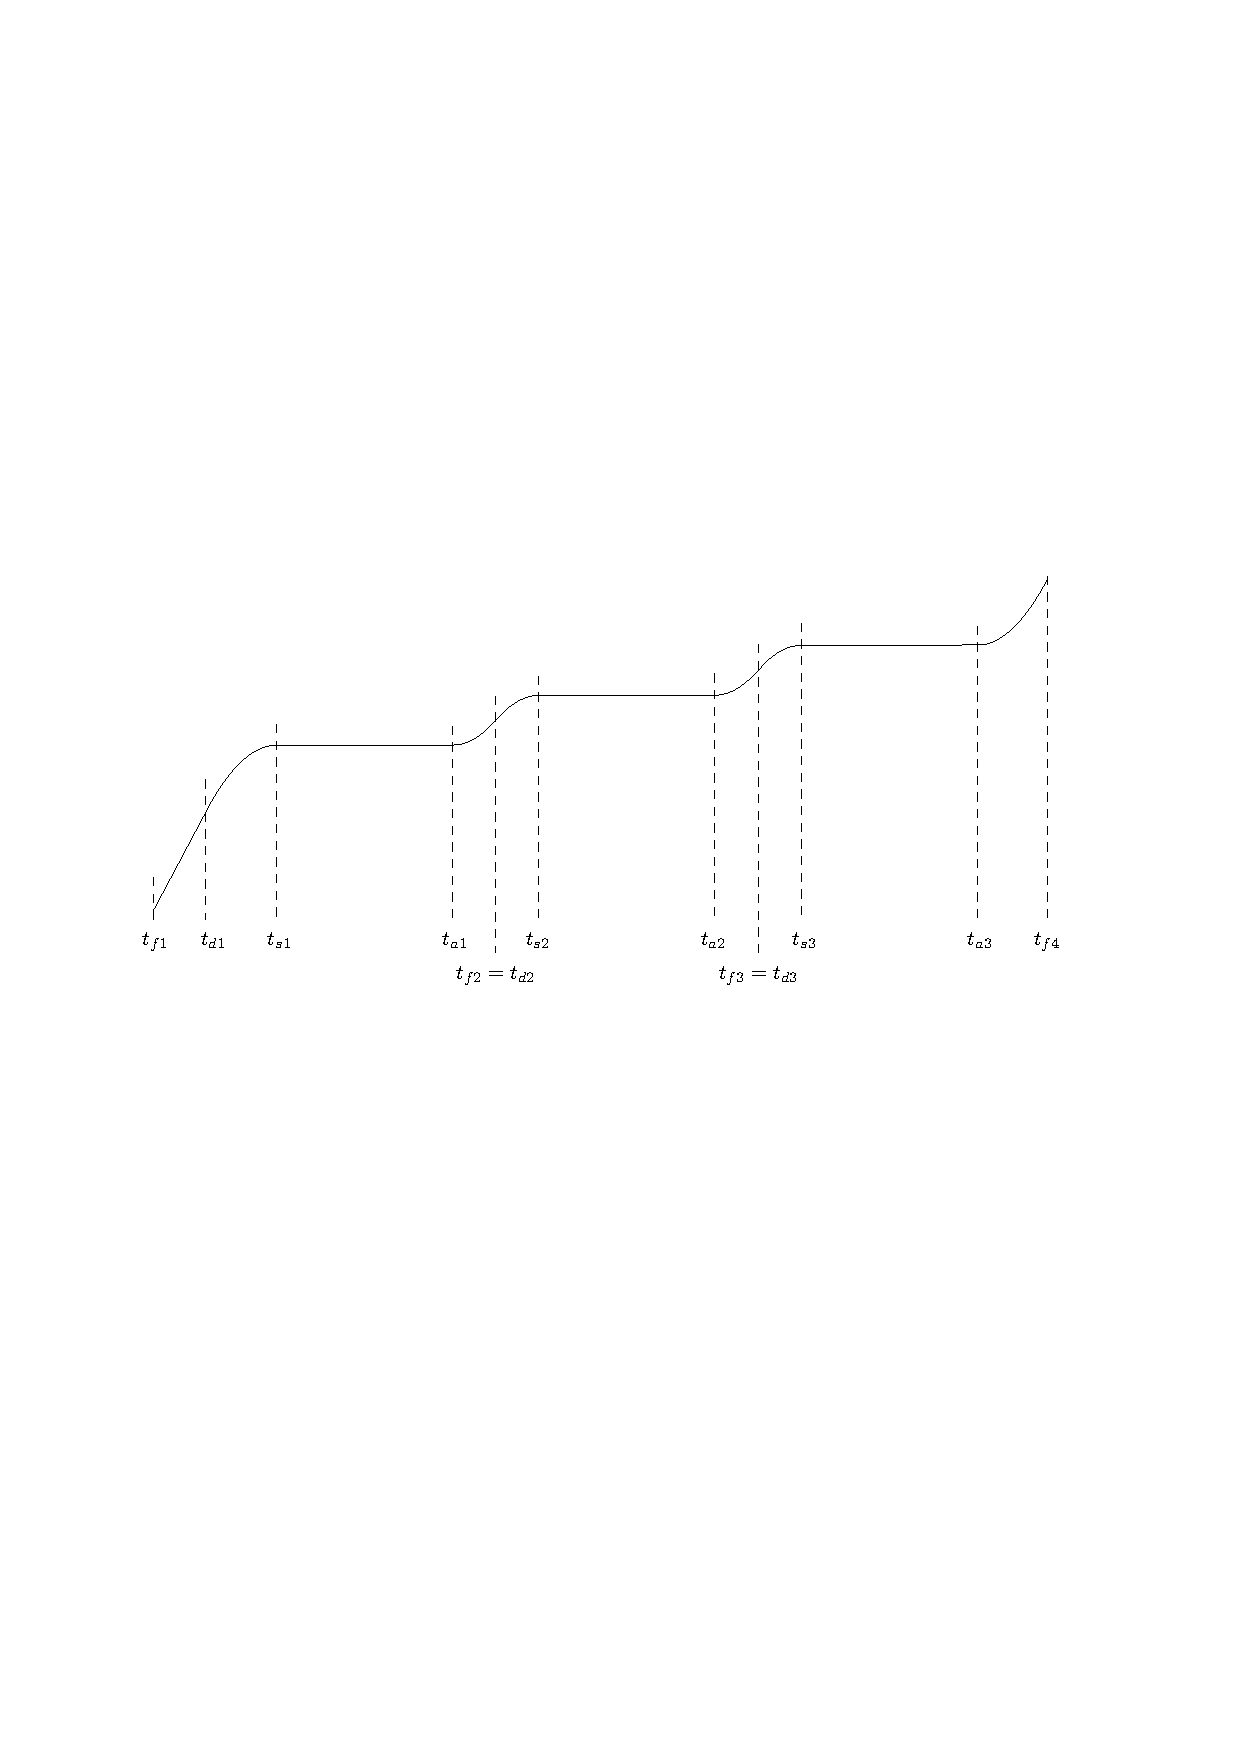
\includegraphics[width=0.99\textwidth]{figures/motion/tandem_trajectory}
  \caption{Some example of an alternating vehicle trajectory $x$. The particular
    shape of this trajectory is due to two preceding vehicles, which causes the
    two ``bumps'' at the times where these vehicles exit the lane. The
    trajectory of the current lead vehicle and previous lead vehicles that gave
    rise to this particular shape are not shown for clarity.}
  \label{fig:tandem_trajectory}
\end{figure}

The proof of this result will also show how optimal solutions can be computed.
We will first consider situations in which the lead constraint $h_{2}$ is
inactive, such that it can essentially be ignored. Next, we generalize this
resulting lemma slightly to also allow non-maximal initial velocities
$v_{0} < 1$. This lemma is then used characterize the optimal trajectories of
the original problem with constraint $h_{2}$.


%
% \begin{align*}
%   \max \int_{0}^{T} \underbrace{x_{1}(t)}_{F(x,u,t)} dt
% \end{align*}
% \begin{align*}
%   \dot{x} = f(x,u,t) = \begin{pmatrix} x_{2} \\ u \end{pmatrix} , \quad
%   x(0) = \begin{pmatrix}
%            p_{0} \\ 1
%          \end{pmatrix}
% \end{align*}
% \begin{align*}
%   -a_{\max} \leq u(t) \leq a_{\max} \quad &\iff \quad \underbrace{a_{\max}^{2} - u^{2}}_{g(x,u,t)} \geq 0 \\[1em]
%   0 \leq x_{2}(t) \leq 1 \quad &\iff \quad \underbrace{x_{2} - x_{2}^{2}}_{h(x,t)} \geq 0 \\[1em]
%   x(T) = \begin{pmatrix} 0 \\ 1 \end{pmatrix} \quad &\iff \quad
%   \underbrace{\begin{pmatrix}
%     x_{1}(T) \\ x_{2}(T) - 1
%   \end{pmatrix}}_{b(x(T), T)} = 0
% \end{align*}
%

Since the system dynamics are time-homogeneous, i.e., they do not depend on
time, we can apply Bellman's optimality principle to show optimality of
subproblems as stated in the following result.

\begin{lemma}
  \label{bellman}
  Let $x^{*}: [t_{0}, 0] \rightarrow \openhalf{-\infty}{0}$ be an optimal
  trajectory for problem~\eqref{eq:optimal_control}. For any time $\tau \in [t_{0}, 0]$, consider the subproblem with
  $t_{0}' = t_{0} + \tau$ and $p_{0}' = p_{0} + x^{*}(\tau)$, then Bellman's
  principle of optimality implies that the optimal trajectory is now simply
  given by the truncation of $x^{*}$ to $[\tau, 0]$, which we will denote by
  $x^{*}|_{[\tau, 0]}$.
\end{lemma}


\subsubsection{Inactive lead constraint}
\label{sec:single_vehicle}

We now consider the case when the lead constraint $h_{2}$ can be ignored,
which might occur when the preceding vehicle is sufficiently far away, or the
current vehicle is the only vehicle in the system. In this case, we consider the
problem (\hyperref[eq:setting]{2a}). We prove Theorem~\ref{thm:optimal_control} in this special case
as Lemma~\ref{lemma1} below.
%
% The proof uses a variant of the Pontryagin Maximum Principle, specifically
% tailored to problems with state
% constraints~\cite{hartlSurveyMaximumPrinciples1995}.
%
When dealing with optimal control problems, Pontryagin's Maximum Principle (PMP)
provides a family of necessary conditions for optimality. We are going to apply
such a PMP-style necessary condition that deals with mixed and pure state
constraints to characterize the optimal control.
%
A common approach to deal with pure state inequality constraints $h$ is to
introduce a multiplier $\eta$ and append $\eta h$ to the Hamiltonian, which is known
as the direct adjoining approach. Instead, we use Theorem 5.1 from~\cite{hartlSurveyMaximumPrinciples1995} (see also
equations (4.29) in~\cite{sethiOptimalControlTheory2019}), which is a so-called indirect adjoining approach,
because $\eta h^{1}$ is appended to the Hamiltonian instead, where $h^{1}$ is
defined as
\begin{align*}
  h^{1} = \frac{dh}{dt} = \frac{\partial h}{\partial x}f + \frac{\partial h}{\partial t} .
\end{align*}
%
For our current problem, the first derivative of pure state constraint $h_{1}$
with respect to time $t$ is given by
\begin{align*}
  h_{1}^{1}(x, u, t) = u - 2x_{2} u ,
\end{align*}
which shows that $h_{1}$ is first-order, because the control $u$ appears after
differentiating once.

\begin{lemma}
  \label{lemma1}
  Consider problem~{\normalfont (\hyperref[eq:setting]{2a})} with $v_{0} = 1$.
  Let the acceleration/deceleration duration and the start of the deceleration
  period, respectively, be given by
  \begin{align*}
  d \;&= \, \min\left\{ 1 / \omega, \sqrt{(p_{0} - t_{0}) / \omega} \right\} , \\
  t_{d}\, &= \, \omega d^{2} - 2d + t_{0} -p_{0} .
  \end{align*}
  The problem is feasible if and only if $t_{0} \leq p_{0}$ and $t_{d} \geq 0$ and in
  that case the optimal control function is given by
  \begin{align*}
    u(t) = \begin{cases}
             -\omega & \text{ for } t_{d} < t < t_{d} + d ,\\
             \omega & \text{ for } {-d} < t < 0 , \\
             0 & \text{ otherwise. }
           \end{cases}
  \end{align*}
\end{lemma}
\begin{proof}
The initial velocity is $x_{2}(t_{0}) = 1$, so without any further deceleration,
the earliest possible time of arrival is $t_{0} - p_{0}$, so there is no
feasible control whenever $t_{0} > p_{0}$, showing the necessity of the first
feasibility condition. Whenever we have $t_{0} = p_{0}$, the optimal
controller is simply $u(t) = 0$. In the rest of the proof, we assume that
$t_{0} < p_{0}$. In that case, there needs to be at least one period of
deceleration and thus also at least one period of acceleration to satisfy
the boundary condition $x_{2}(t_{0})=x_{2}(0)=1$.

By adjoining $\mu g + \eta h_{1}^{1}$ to the Hamiltonian
$H(x, u, \lambda, t) = F(x,u,t) + \lambda f(x,u,t)$ we obtain the Lagrangian in so-called
Pontryagin form
\begin{align*}
  L(x, u, \lambda, \mu, \eta, t) &= H(x, u, \lambda, t) + \mu g(x, u, t) + \eta h_{1}^{1}(x, u, t) \\
  &= x_{1}  + \lambda_{1}x_{2} + \lambda_{2}u + \mu(\omega^{2} - u^{2}) + \eta(u - 2x_{2}u) .
\end{align*}
%
Let $\{ x^{*}(t), u^{*}(t) \}$ denote an optimal pair for problem~(\hyperref[eq:setting]{2a}),
which must satisfy the necessary conditions in Theorem~5.1 from~\cite{hartlSurveyMaximumPrinciples1995}.
%
The Hamiltonian maximizing condition requires
\begin{align*}
  \lambda_{2}u^{*}(t) \geq \lambda_{2} u \quad \text{ at each } t \in [t_{0}, 0] ,
\end{align*}
for all $-\omega \leq u \leq \omega$ such that $u - 2x^{*}_{2}u \geq 0$
whenever $x_{2}^{*} = 0$ or $x_{2}^{*} = 1$. Hence, the optimal controller must
satisfy
\begin{align}
  \label{eq:optimal_u}
  \begin{split}
  u^{*}(t) =
  \begin{cases}
  -\omega &\text{ when } \lambda_{2}(t) < 0, \; x^{*}_{2}(t) > 0 , \\
  \omega &\text{ when } \lambda_{2}(t) > 0, \; x^{*}_{2}(t) < 1 , \\
  0 &\text{ otherwise. }
  \end{cases}
  \end{split}
\end{align}

Observe that the Lagrange multipliers $\mu(t)$ and $\eta(t)$ must satisfy the
complementary slackness conditions
\begin{align*}
  \mu (\omega^{2} - {(u^{*})}^{2}) = 0 ,& \quad \mu \geq 0 , \\
  \eta (x_{2} - x_{2}^{2}) = 0 ,& \quad \eta \geq 0 \; \text{ and } \; \dot{\eta} \leq 0 .
\end{align*}
%
Whenever $u^{*} \neq 0$ on any open interval, then it is clear that we must have
$0 < x_{2} < 1$ on that interval, so the second complementary slackness
condition requires that we have $\eta = 0$. Hence, we have $\eta u^{*} = 0$
almost everywhere.
%
Next, we investigate the costate trajectory $\lambda$, which must satisfy the adjoint
equations
\begin{align*}
  \dot{\lambda} = - L_{x}(x^{*}, u^{*}, \lambda, \mu, \eta, t) \iff
  \begin{cases}
    \dot{\lambda_{1}} = -1 , \\
    \dot{\lambda_{2}} = - \lambda_{1} + 2 \eta u^{*} = -\lambda_{1} ,
  \end{cases}
\end{align*}
%
so we have $\dot{\lambda_{2}}(t) = t + c_{1}$ and
$\lambda_{2}(t) = \frac{1}{2}t^{2} + c_{1}t + c_{2}$ for some constants
$c_{1}, c_{2}$.
%
In view of~\eqref{eq:optimal_u} and the initial condition $x_{2}(t_{0}) = 1$, this shows that
$u^{*}(t)$ has at most one period of deceleration and at most one period of
acceleration.
%
As we argued above, we need at least one period of deceleration and
acceleration, so $\lambda_{2}(t)$ must have exactly two zeros. Let $t_{d}$ and $t_{a}$
denote the start of the deceleration and acceleration periods, respectively.
%
We show that these are uniquely determined by the necessary optimality
conditions when the problem is feasible, fixing a unique optimal control
function $u^{*}(t)$.
%
Let $d \geq 0$ denote the duration of the deceleration, which is also the duration
of the acceleration, because of the boundary conditions
$x_{2}(t_{0}) = x_{2}(0) = 1$. Observe that $d \leq 1 / \omega$ to satisfy velocity
constraint $h_{1}$.

First, we show that $t_{a}$ is uniquely determined in terms of $d$, using the
necessary condition
\begin{align}
  \label{eq:Lu}
  \frac{\partial L}{\partial u} |_{u=u^{*}(t)} = 0 \iff \lambda_{2} - 2 \mu u^{*} - 2 \eta x_{2}^{*} + \eta = 0 .
\end{align}
Suppose $t_{a} + d < 0$, which means $d = 1 / \omega$, then for
$t \in (t_{a} + 1 / \omega, 0)$, we have $x_{2}^{*}(t) = 1$ and $u^{*}(t) = 0$, so the
complementary slackness conditions require $\mu(t) = 0$, such that the necessary
condition gives $\lambda_{2}(t) = \eta(t)$. But this would mean that we have
$\dot{\eta}(t) = \dot{\lambda_{2}}(t) > 0$, which contradicts the necessary condition
$\dot{\eta}(t) \leq 0$, hence $t_{a} = - d$.
% \begin{align*}
%   \mu(t) = 0 \; & \text{ for } t \in (0, t_{d}) , \\
%   \eta(t) = 0 \;& \text{ for } t \in (t_{d}, t_{d} + d) , \\
%   \mu(t) = 0 \; & \text{ for } t \in (t_{d} + d, t_{a}) , \\
%   \eta(t) = 0 \;& \text{ for } t \in (t_{a}, t_{a} + d) , \\
%   \mu(t) = 0 \; & \text{ for } t \in (t_{a} + d, T) .
% \end{align*}
% \begin{align*}
%   \lambda_{2}(t) = \eta(t) \; & \text{ for } t \in (0, t_{d}) , \\
%   \lambda_{2}(t) = -2 \mu(t) \; & \text{ for } t \in (t_{d}, t_{d} + d) , \\
%   \lambda_{2}(t) = -\eta(t) \; & \text{ for } t \in (t_{d} + d, t_{a}) , \\
%   \lambda_{2}(t) = 2 \mu(t) \; & \text{ for } t \in (t_{a}, t_{a} + d) , \\
%   \lambda_{2}(t) = \eta(t) \;& \text{ for } t \in (t_{a} + d, T) .
% \end{align*}

Next, we show that $t_{d}$ is uniquely defined in terms of $d$.
%
Because the vehicle drives at full velocity initially, we have
$x_{1}^{*}(t_{d}) = p_{0} + t_{d}$.
%
During deceleration, the vehicle moves exactly $p^{-}(d ; 1) = p^{-}(d)$, so we have
\begin{align*}
  x_{1}^{*}(t_{d} + d) &= x_{1}^{*}(t_{d}) + p^{-}(d) \\
  &= p_{0} + t_{d} - t_{0} + d - \omega d^{2} / 2 .
\end{align*}
%
The vehicle is stationary in between $t_{d} + d$ and $t_{a}$, so we have
$x^{*}(t_{a}) = x^{*}(t_{d} + d)$. Observe that the vehicle moves the same distance
$p^{+}(d; 1 - \omega d) = p^{-}(d)$ during acceleration due to the symmetric
control bounds, which yields
\begin{align*}
  0 = x_{1}^{*}(0) &= x_{1}^{*}(t_{a}) + p^{-}(d) \\
                   &= p_{0} + t_{d} - t_{0} + 2 p^{-}(d) \\
                   &= p_{0} + t_{d} - t_{0} + 2d - \omega d^{2} .
\end{align*}
%
Hence, we have $t_{d} = \omega d^{2} - 2d + t_{0} - p_{0}$.
%which satisfies $t_{d} \leq -p_{0} \leq T$ and $t_{d} \geq 0$ for any $d$

Finally, we show that $d$ is uniquely determined whenever the problem is feasible.
%
Observe that $d$ determines a feasible control if and only if $0 \leq t_{d}$ and
$t_{d} + d \leq t_{a}$, where the last inequality must be equality whenever
$d < 1 / \omega$ in order to satisfy~\eqref{eq:optimal_u}.
%
Using the definitions of $t_{d}$ and $t_{a}$, inequality $t_{d} + d \leq t_{a}$
can be rewritten to
\begin{align}
  \label{eq:d_eq}
  d^{2} \leq (p_{0} - t_{0}) / \omega .
\end{align}
Suppose the problem has $1/ \omega^{2} \leq (p_{0} - t_{0}) / \omega$, and suppose
$d < 1/ \omega$, then $d^{2} < 1/\omega^{2} \leq (p_{0} - t_{0}) / \omega$, which is
not allowed by~\eqref{eq:optimal_u}, so $d = 1/ \omega$.
%
Otherwise, when $1 / \omega^{2} > (p_{0} - t_{0}) / \omega$, then we must have $d < 1/\omega$ and equality in~\eqref{eq:d_eq}, which yields $d = \sqrt{(p_{0} - t_{0}) / \omega}$.
%
Observe that
$1/\omega^{2} \leq (p_{0} - t_{0}) / \omega$ is equivalent to $1/ \omega \leq \sqrt{(p_{0} - t_{0}) / \omega}$,
which allows us to conveniently write these two solutions as a single expression
$d = \min\{1/ \omega, \sqrt{(p_{0} - t_{0}) / \omega}\}$.
\end{proof}

\begin{remark}
  The feasibility constraint $t_{0} \leq p_{0}$ gives a lower bound on the amount
  of time in which the vehicle can travel across the lane to the next
  intersection. Therefore, we will refer to it as the \emph{travel constraint}.
\end{remark}


\begin{lemma}
  \label{lemma3}
  Consider problem~{\normalfont (\hyperref[eq:setting]{2a})} with $v_{0} = 0$.
  Define the candidate durations
  \begin{align*}
    a^{(1)} &= \sqrt{-p_{0} / \omega - 1/2\omega^{2}} , \\
    a_{1}^{(2)} &= \frac{p_{0} + 1/2\omega}{1 + t_{0}\omega} - \frac{1 + t_{0}\omega}{4 \omega} , \\
    d^{(2)} &= -t_{0}/2 - 1/2\omega , \\
    a_{2}^{(2)} &= -a_{1}^{(2)} + 1/2\omega - t_{0}/2 .
  \end{align*}
  % \begin{align*}
  %   \alpha &= \sqrt{-p_{0} / \omega - 1/2\omega^{2}} , \\
  %   \beta &= -t_{0}/2 - 1/2\omega , \\
  %   a_{1}^{(2)} &= \beta/2 + \alpha^{2}/2d , \\
  %   a_{2}^{(2)} &= \beta/2 - \alpha^{2}/2d + 1/\omega .
  % \end{align*}
  Furthermore, define the candidate subproblem
  $z_{1} := (t_{1}, p_{1}, 1) := (t_{0} + 1 / \omega, p_{0} + 1/2\omega, 1)$ and let
  $d(z_{1})$ and $t_{d}(z_{1})$ denote the duration and start, respectively, of
  the deceleration period as given by Lemma~{\normalfont\ref{lemma1}} for subproblem
  $z_{1}$. Problem {\normalfont (\hyperref[eq:setting]{2a})} is feasible if and
  only if $t_{0} \leq -1/\omega$ and $p_{0} \leq -1/2\omega$ and one of the cases holds
  in the definition
  \begin{align*}
    (a_{1},t_{d},d,a_{2}) := \begin{cases}
              (1 / \omega, t_{1} + t_{d}(z_{1}), d(z_{1}), d(z_{1})) & \text{ if } \, t_{1} \leq p_{1} \text{ and } \; t_{d}(z_{1}) \geq 0 , \\
                               (a^{(1)}, t_{0} + a^{(1)}, a^{(1)}, 1/\omega) & \text{ if }  a^{(1)} \in [0, 1/\omega] \text{ and }  a^{(1)} < d^{(2)} , \\
              (a_{1}^{(2)}, t_{0} + a_{1}^{(2)}, d^{(2)}, a_{2}^{(2)}) & \text{ if } a_{1}^{(2)}, d^{(2)}, a_{2}^{(2)} \in [0, 1/\omega] ,
            \end{cases}
  \end{align*}
  and in that case, the optimal control function is given by
  \begin{align*}
    u(t) = \begin{cases}
             \omega & \text{ for } t_{0} < t < t_{0} + a_{1} , \\
             -\omega & \text{ for } t_{d} < t < t_{d} + d ,\\
             \omega & \text{ for }  {-a_{2}} < t < 0 , \\
             0 & \text{ otherwise. }
           \end{cases}
  \end{align*}
\end{lemma}
\begin{proof}
  The necessary optimality conditions of the current problem lead to the same
  Hamiltonian maximization condition and adjoint equations as in
  Lemma~\ref{lemma1}. Since $v_{0} = 0$, there must be at least one acceleration
  period, followed by an optional deceleration and an optional acceleration. Let
  $a_{1}, d, a_{2}$ denote the durations of these three periods, respectively.
  %
  From~\eqref{eq:optimal_u} follows that the first acceleration happens on
  $(t_{0}, t_{0} + a_{1})$. From~\eqref{eq:Lu} follows that the second
  acceleration must happen on $(-a_{2}, 0)$, by the same argument as in
  Lemma~\ref{lemma1}. Let $t_{d}$ denote the start of the deceleration period.
  Furthermore, let $s_{1} := t_{d}-t_{0}-a_{1}$ and $s_{2} := -a_{2}-t_{d}-d$ denote
  the times between the two consecutive pairs of period, such that
  $t_{0} + a_{1} + s_{1} + d + s_{2} + a_{2} = 0$.
  %
  Suppose that $t_{0} > -1/\omega$, then any trajectory satisfies $x_{2}(0) < 1$,
  which is infeasible, so the first feasibility condition is necessary.
  % Observe that the earliest time of arrival $t_{e}$ can only be achieved when
  % $a_{1} = \min\{ 1/\omega, -t_{0} \}$ and $d=a_{2}=0$. In that case, we have
  % $x_{2}(t) = 1$ for every $t \in (t_{0} + a_{1}, 0)$, which yields
  % $t_{e} = a_{1} - p^{+}(a_{1}) - p_{0}$.
  Observe that any trajectory must accelerate for a duration of at least
  $1/\omega$, which causes a displacement of at least
  $p^{+}(1/\omega) = 1/2\omega$. Hence, a feasible trajectory only exists if
  $p_{0} \leq -1/2\omega$.

  \vspace{0.5em}
  \noindent
  \textit{Full first acceleration.}\;
  Suppose there exists a trajectory $x$ with $a_{1} = 1/\omega$. In this case, we can
  leverage Lemma~\ref{lemma1} as follows. Observe that $x_{2}(t_{1}) = 1$, so
  due to Lemma~\ref{bellman}, the truncated trajectory $x|_{[t_{1}, 0]}$ is a solution to
  subproblem $z_{1} = (t_{1}, x_{1}(t_{1}), 1)$. Therefore, $z_{1}$ must satisfy
  the two feasibility conditions of Lemma~\ref{lemma1}. Furthermore, we must have
  $a_{2} = d$.

  Next, we show that when a trajectory $x$ exists with $a_{1} = 1/\omega$, then
  there cannot exist another feasible trajectory with $a_{1} < 1/\omega$ that
  satisfies the necessary optimality conditions, so $x$ must be optimal.
  %
  Assume there exists an optimal trajectory $x'$ with $a_{1}' < 1 / \omega$, then
  $s_{1}' = 0$ and $d' \leq a_{2}'$.
  %
  First, suppose $x$ is such that $d = 1/ \omega$, then the total travel distance satisfies
  \begin{align*}
    x_{1}'(0) &= p_{0} + p^{+}(a_{1}') + p^{-}(d') + p^{+}(a_{2}') \\
              &< p_{0} + p^{+}(1/\omega) + s_{1} + p^{-}(1/\omega) + p^{+}(1/\omega) = x_{1}(0) = 0,
  \end{align*}
  which shows that $x'$ is infeasible.
  %
  Otherwise, $x$ is such that $d < 1/\omega$, so $s_{2} = 0$. First, we show that
  $a_{2}' > d$, which holds trivially when $s_{2}' > 0$, because then we have
  $a_{2}' = 1/\omega$. When $s_{2}' = 0$, we derive it using
  \begin{align}
    \begin{split}
    \label{eq:time_equal}
    &t_{0}+ a_{1}' + d' + a_{2}' = t_{0} + a_{1} + s_{1} + 2d = 0 , \\
    &\; \implies 2a_{2}' \geq d' + a_{2}' > s_{1} + 2d \geq 2d .
    \end{split}
  \end{align}
  %
  It also follows from~\eqref{eq:time_equal} that
  $t_{2} := t_{0} + a_{1}' + d' < t_{0} + a_{1} + d$. Because $a_{1}' < a_{1}$,
  we have $x_{1}'(t_{2}) < x_{1}(t_{2})$. Furthermore, we have
  $x_{1}'(-a_{2}') > x_{1}(- a_{2}')$.
  %
  But this leads to the contradiction
  \begin{align}
    \label{eq:contradiction}
    x_{1}'(t_{2}) < x_{1}(t_{2}) \leq x_{1}(-a_{2}') < x_{1}'(- a_{2}') = x_{1}'(t_{2}) .
  \end{align}

\begin{figure}
  \centering
  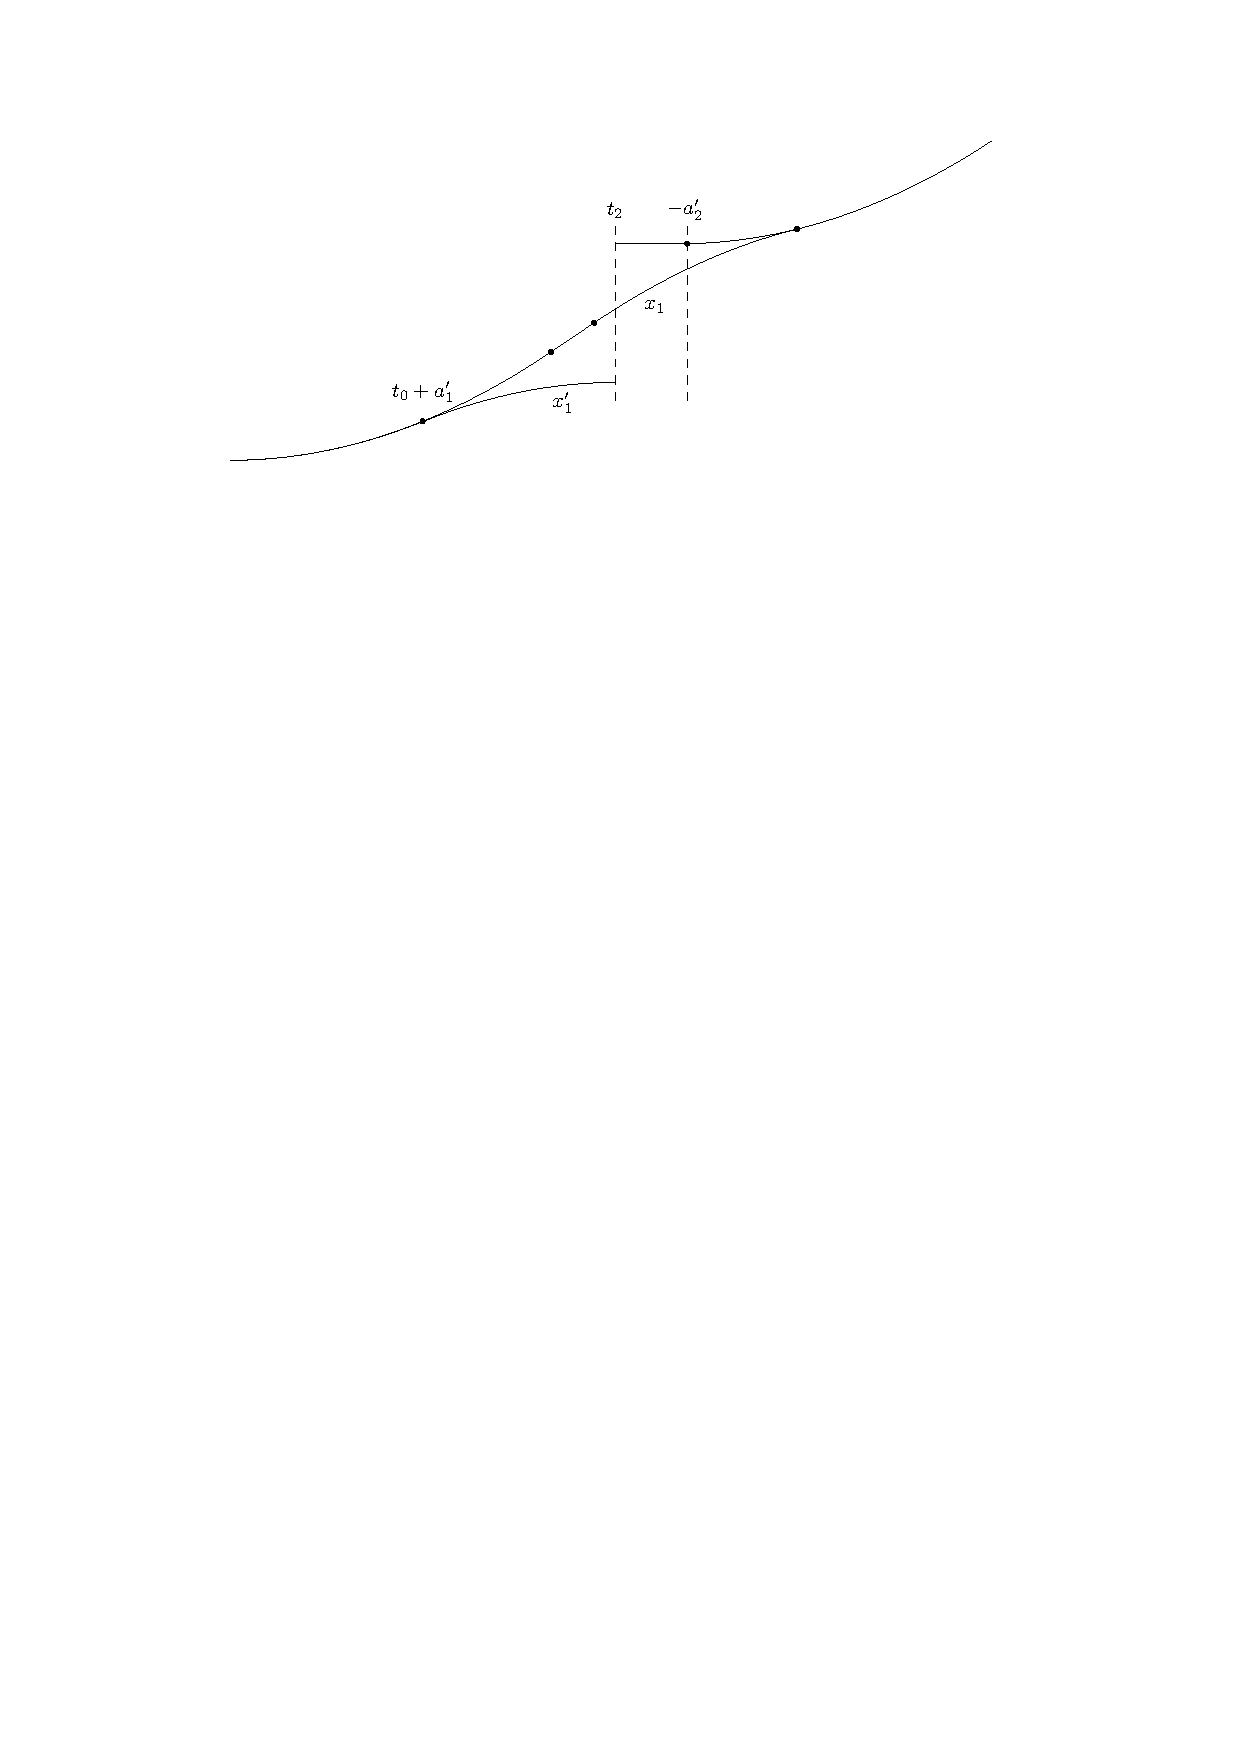
\includegraphics[width=0.80\textwidth]{figures/motion/lemma3_proof1}
  \caption{Illustration of contradiction~\eqref{eq:contradiction} for proving
    that a trajectory $x'$ with $a_{1}' < 1/\omega$ does not exist when a
    trajectory $x$ exists with full first acceleration $a_{1} = 1/\omega$. The
    dots mark the control switching times for both trajectories. Hence, the
    left-most and right-most dot correspond to an inflection point of $x'$ and
    $x$, respectively.}
  \label{fig:lemma3_proof1}
\end{figure}


  \vspace{0.5em}
  \noindent
  \textit{Partial first acceleration.}\; Suppose there exists a trajectory $x$ with
  $a_{1} < 1 / \omega$, then $s_{1} = 0$ and $t_{d} = t_{0} + a_{1}$. First, suppose
  $s_{2} > 0$, then $d = a_{1}\in [0, 1/\omega]$ and $a_{2} = 1/ \omega$, so this
  happens if only if $t_{0} + 2a_{1} + 1/\omega < 0$, which is equivalent to
  $a_{1} < d^{(2)}$.
  %
  Due to the symmetric control bounds, we have
  $p^{+}(a_{1}) = p^{-}(a_{1};\omega a_{1})$ and we can find $a_{1}$ using the
  total travel distance equation
  \begin{align*}
    0 = x_{1}(0) &= p_{0} + 2p^{+}(a_{1}) + p^{+}(1/\omega) \\
    % &= p_{0} + \omega a_{1}^{2} + 1 / 2\omega \\
    &\implies a_{1} = \sqrt{-p_{0} / \omega - 1/2\omega^{2}} .
  \end{align*}

  Next, suppose $s_{2} = 0$, then $a_{1},d,a_{2} \in [0, 1/\omega]$ can be
  determined by solving a system of three equations. We have the total time
  equation $t_{0} + a_{1} + d + a_{2} = 0$ and the total acceleration equation
  $a_{1} - d + a_{2} = 1 / \omega$, from which we can derive
  \begin{align*}
    a_{1} + a_{2} &= d + 1/\omega = -t_{0} - d  \\
    % &\implies t_{0} + 2d = -1/\omega \\
    &\implies d = -1/2\omega - t_{0}/2 \\
    &\implies a_{2} = -a_{1} + 1/2\omega - t_{0}/2.
  \end{align*}
  %
  We can find $a_{1}$ from the total travel distance equation
  \begin{align*}
    0 = x_{1}(0) &= p_{0} + p^{+}(a_{1}) + p^{-}(d; \omega a_{1}) + p^{+}(a_{2}; \omega (a_{1} - d)) \\
      % &= p_{0} + \omega a_{1}^{2}/2 + \omega a_{1} d - \omega d^{2} /2 + \omega(a_{1} - d)a_{2} + \omega a_{2}^{2} / 2 \\
      % &= p_{0} + (\omega / 2) (a_{1}^{2} + a_{2}^{2} + 2a_{1}a_{2} + 2d(a_{1}- a_{2}) - d^{2}) \\
      % &= p_{0} + (\omega / 2) ((a_{1} + a_{2})^{2} + 2d(2 a_{1} + t_{0}  + d) - d^{2}) \\
      % &= p_{0} + (\omega / 2) ((d + 1/\omega)^{2} + 4d a_{1} + 2d t_{0}  + d^{2}) \\
      % &\implies 4d a_{1} = \frac{-2p_{0}}{\omega} - (d+1/\omega)^{2}  - 2d t_{0}  - d^{2} \\
      % &\implies a_{1} = \frac{-p_{0}}{2 \omega d} - \frac{(d+1/\omega)^{2}}{4d}  - t_{0}/2  - d/4 \\
      % &\quad = \frac{-p_{0}}{2\omega d} - \frac{d + t_{0} + 1/\omega}{2} - \frac{1}{4d\omega^{2}} \\
      % &\quad = \frac{p_{0} + 1/2\omega}{1 + t_{0}\omega} - \frac{1 + t_{0}\omega}{4 \omega} .
    &\implies a_{1} = \frac{p_{0} + 1/2\omega}{1 + t_{0}\omega} - \frac{1 + t_{0}\omega}{4 \omega} .
  \end{align*}
  % Finally, observe that in order for $a_{1}^{(2)}, d^{(2)}, a_{2}^{(2)}$ to
  % define a feasible trajectory, they must each lie in the interval
  % $[0, 1/\omega]$.
  % However, from the feasibility condition $t_{0} \leq -1/\omega$, it already follows
  % that $d^{(2)} \geq 0$ and $a^{(2)} \geq 0$, so we only include the remaining
  % inequalities as feasibility conditions.


  Finally, we show that when a trajectory $x$ exists such that
  $a_{1} < 1/\omega$ and $s_{2} > 0$, we show that there cannot exist another
  optimal trajectory $x'$ with $s_{2}' = 0$.
  %
  Suppose such $x'$ exists, then it satisfies $a_{1}' < 1/\omega$, as shown in the
  previous section of the proof. Therefore, we have
  $(a_{1}', d', a_{2}') = (a_{1}^{(2)}, d^{(2)}, a_{2}^{(2)})$, so feasibility
  of $x'$ implies $a_{2}^{(2)} = a_{1}' \leq 1/\omega$.
  %
  It is straightforward to verify that this inequality can be rewritten to
  \begin{align*}
    a_{2}^{(2)} &= d^{(2)}/2 - (a^{(1)})^{2}/2d^{(2)} + 1/\omega  \leq 1/\omega ,
  \end{align*}
  from which we derive that $a^{(1)} \geq d^{(2)}$. However, this contradicts
  $a^{(1)} = a_{1} < d^{(2)}$, which must hold because we assumed that $x$ was such that
  $s_{2} > 0$.
\end{proof}

% \begin{lemma}
%   \label{lemma2}
%   Consider problem~{\normalfont (\hyperref[eq:setting]{2a})} with
%   $0 \leq v_{0} < 1$. Let $\alpha = (1-v_{0}) / \omega$ be the maximum initial
%   acceleration duration and define
%   \begin{align*}
%     p_{0}(a) &= p_{0} + p^{+}(a; v_{0}) - p^{-}(\alpha - a) , \\
%     T(a) &= T - 2 a + \alpha , \\
%    \alpha_{1} &= -\frac{v_{0}}{\omega} \pm \sqrt{\frac{\alpha^{2}}{2} - \frac{\alpha + p_{0}}{\omega}} ,
%     \quad\quad \alpha_{2} = \frac{\alpha + T}{4} + \frac{p_{0} + T}{\omega (\alpha - T)} .
%   \end{align*}
%   Let $d(a)$, $t_{d}(a)$ and $t_{a}(a)$ be as given by Lemma~\ref{lemma1} for
%   $p_{0} \equiv p_{0}(a)$ and $T \equiv T(a)$. Let
%   \begin{align*}
%     a_{1} =
%   \begin{cases}
%   \alpha &\text{ if } \; p_{0}(\alpha) + T(\alpha) \geq 0 \; \text{ and } \; t_{d}(\alpha) \geq 0 , \\
%   \alpha_{1} &\text{ if } \; 1 / \omega < p_{0}(\alpha_{1}) + T(\alpha_{1}), \\
%   \alpha_{2} &\text{ if } \; 0 \leq p_{0}(\alpha_{2}) + T(\alpha_{2}) < 1 / \omega ,
%   \end{cases}
%   \end{align*}
%   %
%   and let $a_{1}$ be undefined if none of the above three conditions holds.
%   Whenever $a_{1}$ is defined, problem~{\normalfont (\hyperref[eq:setting]{2a})}
%   is feasible and the optimal control is given by
%   \begin{align*}
%     u(t) = \begin{cases}
%              \omega & \text{ for }  0 < t < a_{1} , \\
%              -\omega & \text{ for } a_{1} + t_{d}(a_{1}) < t < a_{1} + t_{d}(a_{1}) + d(a_{1}) ,\\
%              \omega & \text{ for }  a_{1} + t_{a}(a_{1}) < t < a_{1} + t_{a}(a_{1}) + d(a_{1}) , \\
%              0 & \text{ otherwise. }
%            \end{cases}
%   \end{align*}

% \end{lemma}

% \paragraph{1.}
% By the Hamiltonian maximization condition, the first acceleration period will
% take as long as possible, which means that the remaining problem from
% $x(a_{1})$ onwards is still feasible. Suppose that $a_{1} = \alpha$, then the
% vehicle travels $p^{+}(a_{1}; v_{0})$ in the first acceleration, so define
% \begin{align*}
%   p_{0}' &= p_{0} + p^{+}(a_{1}; v_{0}) \\
%           &= p_{0} + \alpha v_{0} + \omega \alpha^{2} / 2 , \\
%   T' &= T - \alpha , \\
%   t_{d}' &= -p_{0}' - 2d + \omega d'^{2} .
% \end{align*}
% Because we have $x_{2}(t_{f}) = 1$, we can now apply Lemma~\ref{lemma1} to the
% remaining part of the trajectory. Lemma~\ref{lemma1} now yields
% %
% \begin{align*}
%   a_{2} = d &= \min\left\{ \frac{1}{\omega}, \sqrt{\frac{p_{0}' + T'}{\omega}} \right\} \\
%       &= \min\left\{ \frac{1}{\omega}, \sqrt{\frac{p_{0} + T}{\omega} + \frac{\alpha v_{0} + \omega \alpha^{2} / 2 - \alpha}{\omega}} \right\} \\
%       &= \min\left\{ \frac{1}{\omega}, \sqrt{\frac{p_{0} + T}{\omega} - \frac{\alpha^{2}}{2}} \right\} .
% \end{align*}

% \paragraph{2.}
% Suppose that $a_{1} < \alpha$, then we have
% $s_{1} = 0 \implies x(t_{f}) = x(t_{d})$. Therefore, by computing the total
% distance traveled, we obtain the following equation
% \begin{align}
%   \label{eq:distance_equation}
%   p_{0} + p^{+}(a_{1}; v_{0}) + p^{-}(d; v_{0} + \omega a_{1}) + p^{+}(a_{2}; v_{0} + \omega(a_{1} - d)) = 0 .
% \end{align}
% We now show that this uniquely determines $a_{1}$, by making the following
% case distinction based on $a_{2}$.

% \paragraph{2a.}
% Assume $a_{2} = d_{f}$, then $x_{2}(t_{a}) = v_{0} + \omega(a_{1} - d) = 0$,
% which implies that $a_{1} = d - v_{0} / \omega$.
% Now solving~\eqref{eq:distance_equation} for $d$ yields
% \begin{align*}
%   0 &= p_{0} + p^{+}(a_{1}; v_{0}) + p^{-}(d; v_{0} + \omega a_{1}) + p^{+}(d_{f}; 0) \\
%     &= p_{0} + 1/ 2\omega + v_{0}a_{1} + \omega a_{1}^{2} / 2 + (v_{0} + \omega a_{1}) d - \omega d^{2}/2 \\
%     &= p_{0} + 1/ 2\omega + v_{0}(d - v_{0}/\omega) + \omega(d - v_{0}/\omega)^{2}/2 + v_{0} d + \omega d(d- v_{0}/\omega) - \omega d^{2} / 2 \\
%     &= p_{0} + 1/2\omega + v_{0}d - v_{0}^{2} / \omega + \omega(d^{2}/2 - v_{0} d / \omega + v_{0}^{2} / 2 \omega^{2}) + v_{0}d + \omega d^{2} -v_{0}d - \omega d^{2}/2 \\
%     &= p_{0} + 1/2\omega - v_{0}^{2}/2\omega + \omega d ^{2} \\[0.4em]
%   & \implies d = \sqrt{ \frac{v_{0}^{2} - 1}{2 \omega^{2}} - \frac{p_{0}}{\omega} }  = \sqrt{\frac{\alpha^{2}}{2} - \frac{\alpha + p_{0}}{\omega}}
% \end{align*}

% \paragraph{2b.}
% Assume $a_{2} < d_{f}$, then we have
% \begin{align*}
%   \begin{cases}
%     a_{1} + d + a_{2} = T , \\
%     a_{1} - d + a_{2} = \alpha ,
%   \end{cases}
% \end{align*}
% from which it can be derived that
% \begin{align*}
%   d &= (T - \alpha) / 2 , \\
%   a_{1} &= T  - d - a_{2} = (T + \alpha) / 2 - a_{2} .
% \end{align*}
% Solving~\eqref{eq:distance_equation} for $a_{2}$ yields
% \begin{align*}
%   0 &= p_{0} + v_{0}a_{1} + \omega a_{1}^{2}/2 + (v_{0} + \omega a_{1}) d - \omega d^{2} / 2 + (v_{0} + \omega (a_{1} - d)) a_{2} + \omega a_{2}^{2} / 2 \\
%     &= p_{0} + v_{0} a_{1} + \omega a_{1}^{2} / 2 + v_{0}d + \omega a_{1}d - \omega d^{2} / 2 + v_{0}a_{2} + \omega a_{1}a_{2} -\omega d a_{2} + \omega a_{2}^{2} / 2 \\
%   &= p_{0} + v_{0}T + \omega(a_{1}^{2} + a_{2}^{2} + 2a_{1}a_{2} + 2a_{1}d - 2da_{2} - d^{2}) / 2 \\
%   &= \dots \\
%   &= p_{0} + v_{0}T + \frac{\omega}{2} \left( \left(\frac{T + \alpha}{2}\right)^{2} +2 \left(\frac{T + \alpha}{2}\right)\left(\frac{T - \alpha}{2}\right) - \left(\frac{T - \alpha}{2}\right)^{2} - 4 \left(\frac{T - \alpha}{2}\right) a_{2} \right) \\
%   % &= p_{0} + v_{0}T + \omega((T-d)^{2} + 2a_{1}d - 2da_{2} - d^{2}) / 2 \\
%   % &= p_{0} + v_{0}T + \omega((T-d)^{2} + 2a_{1}d - 2d(T-d-a_{1}) - d^{2}) / 2 \\
%   % &= p_{0} + v_{0}T + \omega((T-d)^{2} + 4a_{1}d - 2d(T-d) - d^{2}) / 2 \\
%   % &= p_{0} + v_{0}T + \omega(T-d)^{2}/2 + 2\omega a_{1}d - \omega d(T-d) - \omega d^{2} / 2 \\
%   % &= p_{0} + v_{0}T + \omega T^{2}/2 - \omega Td + \omega d^{2}/2 + 2\omega a_{1}d - \omega d(T-d) - \omega d^{2} / 2 \\
%   % &= p_{0} + v_{0}T + \omega T^{2}/2 - \omega Td +  2\omega a_{1}d - \omega d(T-d) \\
%   % &= p_{0} + v_{0}T + \omega T^{2}/2 - 2\omega Td +  2\omega a_{1}d - \omega d^{2} \\
%   % &\implies
%   %   a_{1} = \frac{-p_{0} - v_{0}T - \omega T^{2}/2  + 2 \omega Td + \omega d^{2}}{2\omega d}
%   &\iff \frac{p_{0} + T}{\omega} - \frac{\alpha T}{2} + \frac{T-\alpha}{2} (a_{1} - a_{2}) = 0
% \end{align*}


\newpage
\subsubsection{Active lead constraint}

We now consider problem~(\hyperref[eq:setting]{2b}) when lead constraint $h_{2}$
becomes active somewhere along the optimal trajectory. Throughout the following
discussion, let $\bar{x}$ denote the trajectory of the lead vehicle's rear
bumper and assume that there is some control function $\bar{u}$ such that
$\{\bar{x}(\cdot), \bar{u}(\cdot)\}$ is alternating. Let the corresponding switching times
be denoted as $\bar{t}_{\cdot i}$.
%
The lead constraint is of second order, because the control function $u$ only
appears after differentiating twice, as seen in
\begin{align*}
  h_{2}(x, t) &= \bar{x}_{1} - x_{1}, \\
  h_{2}^{1}(x, t) &= \bar{x}_{2} - x_{2}, \\
  h_{2}^{2}(x, u, t) &= \bar{u} - u .
\end{align*}

\vspace{0.5em}
\noindent
\textit{Proof sketch.}
\begin{itemize}
  \item The costate trajectory component $\lambda_{2}$ is exactly like in
        Lemma~\ref{lemma1} when we assume there are no discontinuities, so this
        would violate $h_{2}$, so we must have at least one discontinuity, which
        can only happen at $h_{2}$ entry time.
  \item This discontinuity must take $\lambda_{2}$ from negative to positive.
        This can be used to show that there is only one possible location for
        the discontinuity to happen.
  \item First deceleration must start such that $h_{2}$ is hit. We derive this
        \emph{entry time} $\tau_{1}$, which is later used to formulate our
        so-called \emph{buffer constraints} on the crossing times.
  \item Now given the ``shape'' of the trajectory, we can formulate a system of
        equations to determine the lengths of acceleration/deceleration at the
        end of the trajectory, after the \emph{exit time}.
\end{itemize}



\begin{proof}[\normalfont\textbf{Proof of Theorem}~\ref{thm:optimal_control}]
The Hamiltonian is still the same as in Lemma~\ref{lemma1}, but we need to add a new
term to the Lagrangrian, which is now
\begin{align*}
  L(x, u, \lambda, \mu, \eta_{1}, \eta_{2}, t) &= H(x,u,\lambda,t) + \mu g(x,u,t) + \eta_{1}h_{1}^{1}(x, u, t) + \eta_{2}h_{2}^{2}(x,u,t) \\
  &= x_{1} + \lambda_{1}x_{2} + \lambda_{2} u + \mu(\omega^{2} - u^{2}) + \eta_{1}(u - 2x_{2}u) + \eta_{2}(\bar{u} - u) .
\end{align*}
%
Due to the Hamiltonian maximization principle, the optimal control function
$u^{*}$ must satisfy the following form
\begin{align*}
  \begin{split}
  u^{*}(t) =
  \begin{cases}
  0 &\text{ when } \lambda_{2}(t) > 0, \; x^{*}_{2}(t) = 1 , \\
  0 &\text{ when } \lambda_{2}(t) < 0, \; x^{*}_{2}(t) = 0 , \\
  -\omega &\text{ when } \lambda_{2}(t) < 0, \; x^{*}_{2}(t) > 0 , \\
  \omega &\text{ when } \lambda_{2}(t) > 0, \; x^{*}_{2}(t) < 1, \; x_{1} < \bar{x}_{1} , \\
  \bar{u}(t) &\text{ when } \lambda_{2}(t) > 0, \; x^{*}_{2}(t) < 1, \; x_{1} = \bar{x}_{1} . \\
  \end{cases}
  \end{split}
\end{align*}

The adjoint equations are still the same as in the proof of Lemma~\ref{lemma1}. Hence,
whenever there exists an optimal controller such that $h_{2}$ does never become
active, it is equal to the controller from Lemma~\ref{lemma1}. Therefore, from here on we
assume that constraint $h_{2}$ becomes active, so let the corresponding first \textit{entry time}
be denoted by $\tau_{1}$.
%
We now argue that $\lambda_{2}$ must have a discontinuity at $\tau_{1}$.

\vspace{0.5em}
\noindent
\textit{Before entry time.}\;
First of all, suppose $\tau_{1}$ satisfies
$\bar{t}_{fi} \leq \tau_{1} \leq \bar{t}_{si}$ for some $i$, then we show that
$\tau_{1} = \bar{t}_{fi}$. {\color{Navy} Use Taylor approximation around
  $\tau_{1}$ to show that $\bar{t}_{fi} < \tau_{1} \leq \bar{t}_{si}$ would
  imply that $x_{2} < -\omega$ somewhere, which is not possible.}

Otherwise, suppose $\tau_{1}$ satisfies $\bar{t}_{si} \leq \tau_{1} \leq \bar{t}_{ai}$ for
some $i$, then $x_{2}(\tau_{1}) = \bar{x}_{2}(\tau_{1}) = 0$. This implies that
$u(t) = -\omega$ for $t \in (\tau_{1} - 1/\omega, \tau_{1})$ and $u(t) = 0$ for
$t \in (t_{0}, \tau_{1} - 1/\omega)$. Hence, the position of the entry point
needs to satisfy
\begin{align*}
  \bar{x}_{1}(\bar{t}_{si}) = x_{1}(\tau_{1}) &= p_{0} + \tau_{1} - 1/\omega - t_{0} + p^{-}(1/\omega) \\
                       &= p_{0} + \tau_{1}- t_{0} -1/2\omega ,
\end{align*}
from which we derive that
\begin{align*}
  \tau_{1} = t_{0} - p_{0} + 1/2\omega + \bar{x}_{1}(\bar{t}_{si}) .
\end{align*}
Furthermore, we have $t_{d1} = \tau_{1} - 1/\omega$ in this case.

Otherwise, suppose $\tau_{1}$ satisfies
$\bar{t}_{ai} \leq \tau_{1} \leq \bar{t}_{f,i+1}$ for some $i$, then
$x_{1}(\tau_{1}) = \bar{x}_{1}(\tau_{1}) = \bar{x}_{1}(\bar{t}_{ai}) + p^{+}(\tau_{1} - \bar{t}_{ai}; \bar{x}_{2}(\bar{t}_{ai})) $
and
$x_{2}(\tau_{1}) = \bar{x}_{2}(\tau_{1}) = \bar{x}_{2}(\bar{t}_{ai}) +  (\tau_{1} - \bar{t}_{ai}) \omega$.
This means that the duration of the initial deceleration $d$ must be given by
\begin{align*}
  d = \frac{1 - x_{2}(\tau_{1})}{\omega} = \frac{1 - \bar{x}_{2}(\bar{t}_{ai})}{\omega} - \tau_{1} + \bar{t}_{ai} .
\end{align*}
Observe that, starting from the initial position, the current vehicle drives at full speed for
a duration of $\tau_{1} - d - t_{0}$ before decelerating, so the position of the
entry point is given by
\begin{align*}
   x_{1}(\tau_{1}) &= p_{0} + \tau_{1} - d - t_{0} + p^{-}(d) , \\
          &= p_{0} + \tau_{1} - t_{0} - \omega d^{2} / 2 .
\end{align*}
%
We can find $\tau_{1}$ by equating $x_{1}(\tau_{1}) = \bar{x}_{1}(\tau_{1})$,
which yields the quadratic equation
\begin{align*}
  p_{0} + \tau_{1} - t_{0} - \omega d^{2} / 2 &= \bar{x}_{1}(\bar{t}_{ai}) + \bar{x}_{2}(\bar{t}_{ai})(\tau_{1} - \bar{t}_{ai}) + \omega (\tau_{1} - \bar{t}_{ai})^{2} / 2 , \\
  \implies \tau_{1} &= \bar{t}_{ai} -\frac{\bar{x}_{2}(\bar{t}_{ai})}{\omega} + \frac{1}{\omega} \\
  &\quad\quad - \frac{1}{2}\sqrt{\frac{2}{\omega^{2}} + \frac{2(\bar{x}_{2}(\bar{t}_{ai}))^{2}}{\omega^{2}} + 4\left( \frac{p_{0} - t_{0} - \bar{x}_{1}(\bar{t}_{ai}) + \bar{t}_{ai}(1 + \bar{x}_{2}(\bar{t}_{ai}))}{\omega} \right)} \\
  t_{d1} &= \tau_{1} - d = 2 \tau_{1} - \bar{t}_{ai} + \frac{\bar{x}_{2}(\bar{t}_{ai}) - 1}{\omega} .
\end{align*}

\vspace{0.5em}
\noindent
\textit{After exit time.}\; Now consider the part of the trajectory after
leaving the boundary. We leverage the result from Lemma~\ref{lemma3}.
\end{proof}

We now show how the result of Theorem~\ref{thm:optimal_control} can be used to
compute the trajectories of a sequence of vehicles scheduled to drive through a
lane. We keep $p_{0} = -d(v,w) + W$ fixed.
%
Let the entry and exit times be denoted, respectively, by $y(i, v)$ and
$y(i, w)$, for some vehicle indices $i = 1, \dots, n$. Assume these
\textit{crossing times} $y$ enable a feasible sequence of trajectories $x^{(i)}$.
%
We use $x[t_{0}, p_{0}, \bar{x}_{1}](t)$ to denote the optimal trajectory given
by Theorem~\ref{thm:optimal_control}, evaluated at time $t$. Similarly, we write
$x[t_{0}, p_{0}, \varnothing]$ to denote the solution given by
Lemma~\ref{lemma1}, so when the lead constraint can be ignored.
%
For the very first vehicle that arrives, we compute
\begin{align*}
  x^{(1)}(t) = x[y(1,v)-y(1,w), \; p_{0}, \; \varnothing](t - y(1,w)) .
\end{align*}
For every next vehicle $i \geq 2$, we recursively compute
\begin{align*}
  x^{(i)}(t) = x[y(i,v)-y(i,w), \; p_{0}, \; x_{1}^{(i-1)}(t - y(j,w)) - L](t - y(j, w)) .
\end{align*}
{\color{Navy} Include illustration to support this notation and derivation.
Discuss where these trajectories are actually defined (domain).}


\newpage
\subsection{Feasibility of crossing times}

\begin{theorem}
  Given crossing times $y(i, v)$ and $y(i, w)$, there exists a feasible
  trajectory $x$ if and only if the crossing times satisfy the follow constraints
  $y(i, v) \geq y(i-1, v) + \rho$ and $y(i, w) \geq y(i-1, w) + \rho$ and buffer constraint $y(i, v) \geq \dots$ and
  travel constraint $y(i, v) + p_{0} \leq y(i, w)$.
\end{theorem}
\begin{proof}
  Argue travel constraint. Argue follow constraint. Rest is for buffer constraint.

\vspace{0.5em}
\noindent
\textit{Necessary.}\;
  Consider crossing times $y(i, v)$ and define
  $t_{a} := y(i - c(v,w), w) - 1/\omega$ and $t_{d} := t_{a} + \min\{1/\omega, \sqrt{L/\omega}\}$.

\vspace{0.5em}
\noindent
\textit{Sufficient.}\;
\end{proof}

\begin{figure}
  \centering
  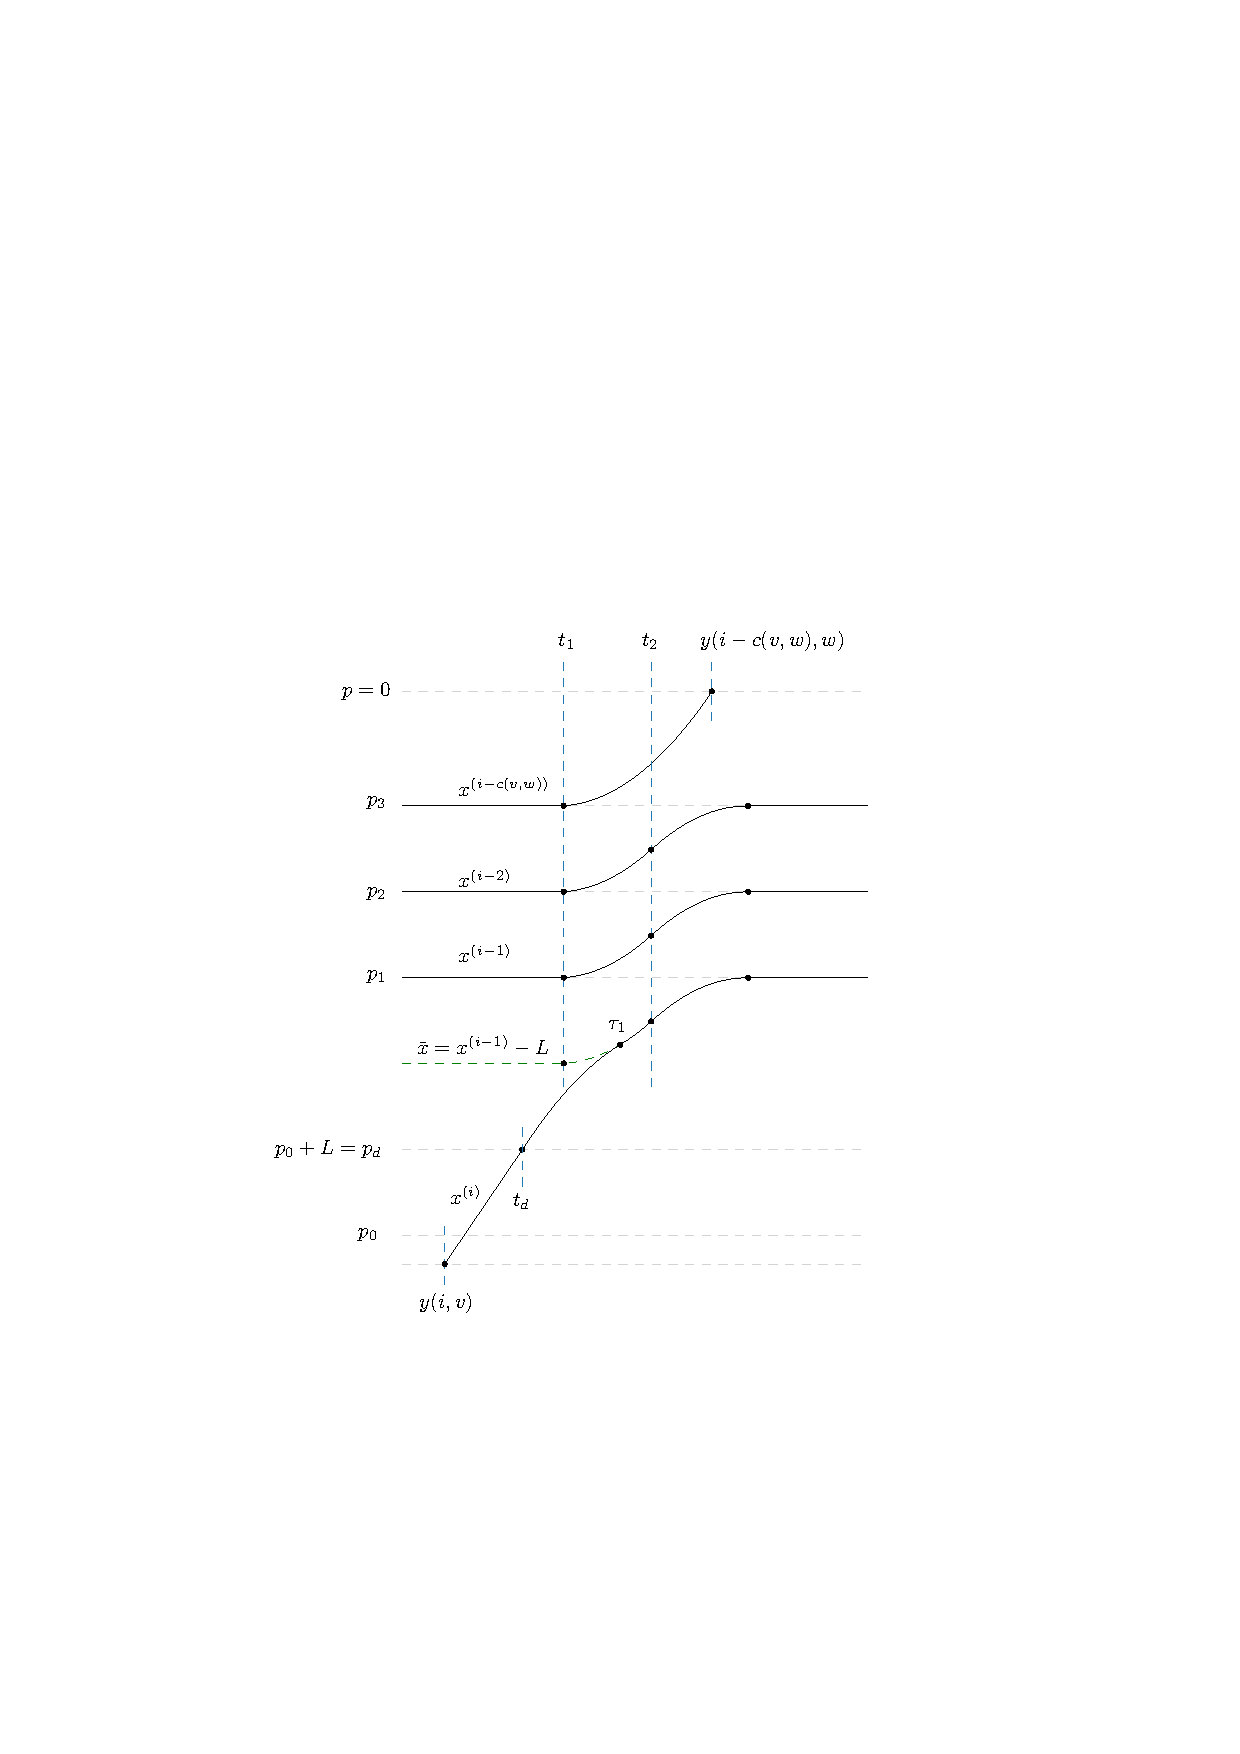
\includegraphics[scale=1]{figures/motion/example1}
  \caption{Example with stationary capacity $c(v,w) = 3$.}
\end{figure}

We now investigate the limit on the number of vehicles that can occupy the lane
when waiting. Imagine that vehicles enter the lane until it is full and then
only after all vehicles have come to a full stop, they start to leave the lane
by crossing $w$. We refer to the maximum number of vehicles that can wait in the
lane as the \textit{stationary lane capacity}.
%
Suppose that we want to design the tandem network that has a stationary lane
capacity of at least $c(v,w)$. Vehicles are required to drive at full speed as
long as they occupy any intersection. Therefore, a vehicle crossing $v$ can only
start decelerating after $p(t) \geq p_{0} + L$, so the earliest position where a
vehicle can come to a stop is $p_{0} + L + p^{+}(d_{f})$.
%
Because vehicles need to gain maximum speed before reaching $w$,
the position closest to $w$ where a vehicle can wait is $- p^{+}(d_{f})$.
%
Hence, in order to accomodate for $c(v,w)$ waiting vehicles, the length of the
lane must satisfy
\begin{align*}
  d(v, w) \geq W + L + 2p^{+}(d_{f}) + (c(v,w) - 1) L ,
\end{align*}
as illustrated in Figure~\ref{fig:tandem_annotated}.
%
Conversely, given the lane length $d(v,w)$, the corresponding stationary lane
capacity is given by\footnote{Without Assumption~\ref{assump:same_geometry}, we
  cannot derive such a simple formula, because it would depend on the specific
  lengths of those vehicles currently in the system.}
\begin{align*}
  c(v, w) = \texttt{floor}\left( \frac{d(v,w) - W - 2 p^{+}(d_{f})}{L} \right) ,
\end{align*}
where $\texttt{floor}(x)$ denotes the largest integer smaller than or equal to
$x$.

{\color{Navy}
% emphasize fixed locations
It turns out that the fixed locations where vehicles wait in the above scenario
are helpful in describing the optimal trajectories, even when vehicles never
fully stop. We will denote these fixed \textit{waiting positions} as
\begin{align*}
  p_{k} = - p^{*}(d_{f}) - (c(v,w) - k) L,
\end{align*}
for $k = 1, \dots, c(v,w)$.
%
Furthermore, let $p_{d} = p_{1} - p^{*}(d_{f})$ denote the position from
which vehicles must decelerate in order to stop at the first waiting position
$p_{1}$.
%
Now consider a vehicle that moves from $p_{k}$ to the next waiting position
$p_{k+1}$, so it moves exactly distance $L$. We consider such a start-stop
movement, without considering any safe following constraints. By symmetry of the
control constraints, the vehicle moves the same distance during both
acceleration and deceleration. Furthermore, the vehicle needs to be at rest at
the start and end of such trajectory. Hence, it is clear that it takes the same
amount of time $d_{s}$ to accelerate and decelerate. We assume that
$d_{s} < d_{f}$, which ensures that maximum velocity is never reached during the
start-stop movement, which is illustrated in Figure~\ref{fig:start-stop}. In this case, it is
clear that we must have $L = 2 p^{*}(d_{s})$, from which we derive that
$d_{s} = \sqrt{L / a_{\max}}$.
}


% \begin{figure}
%   \centering
%   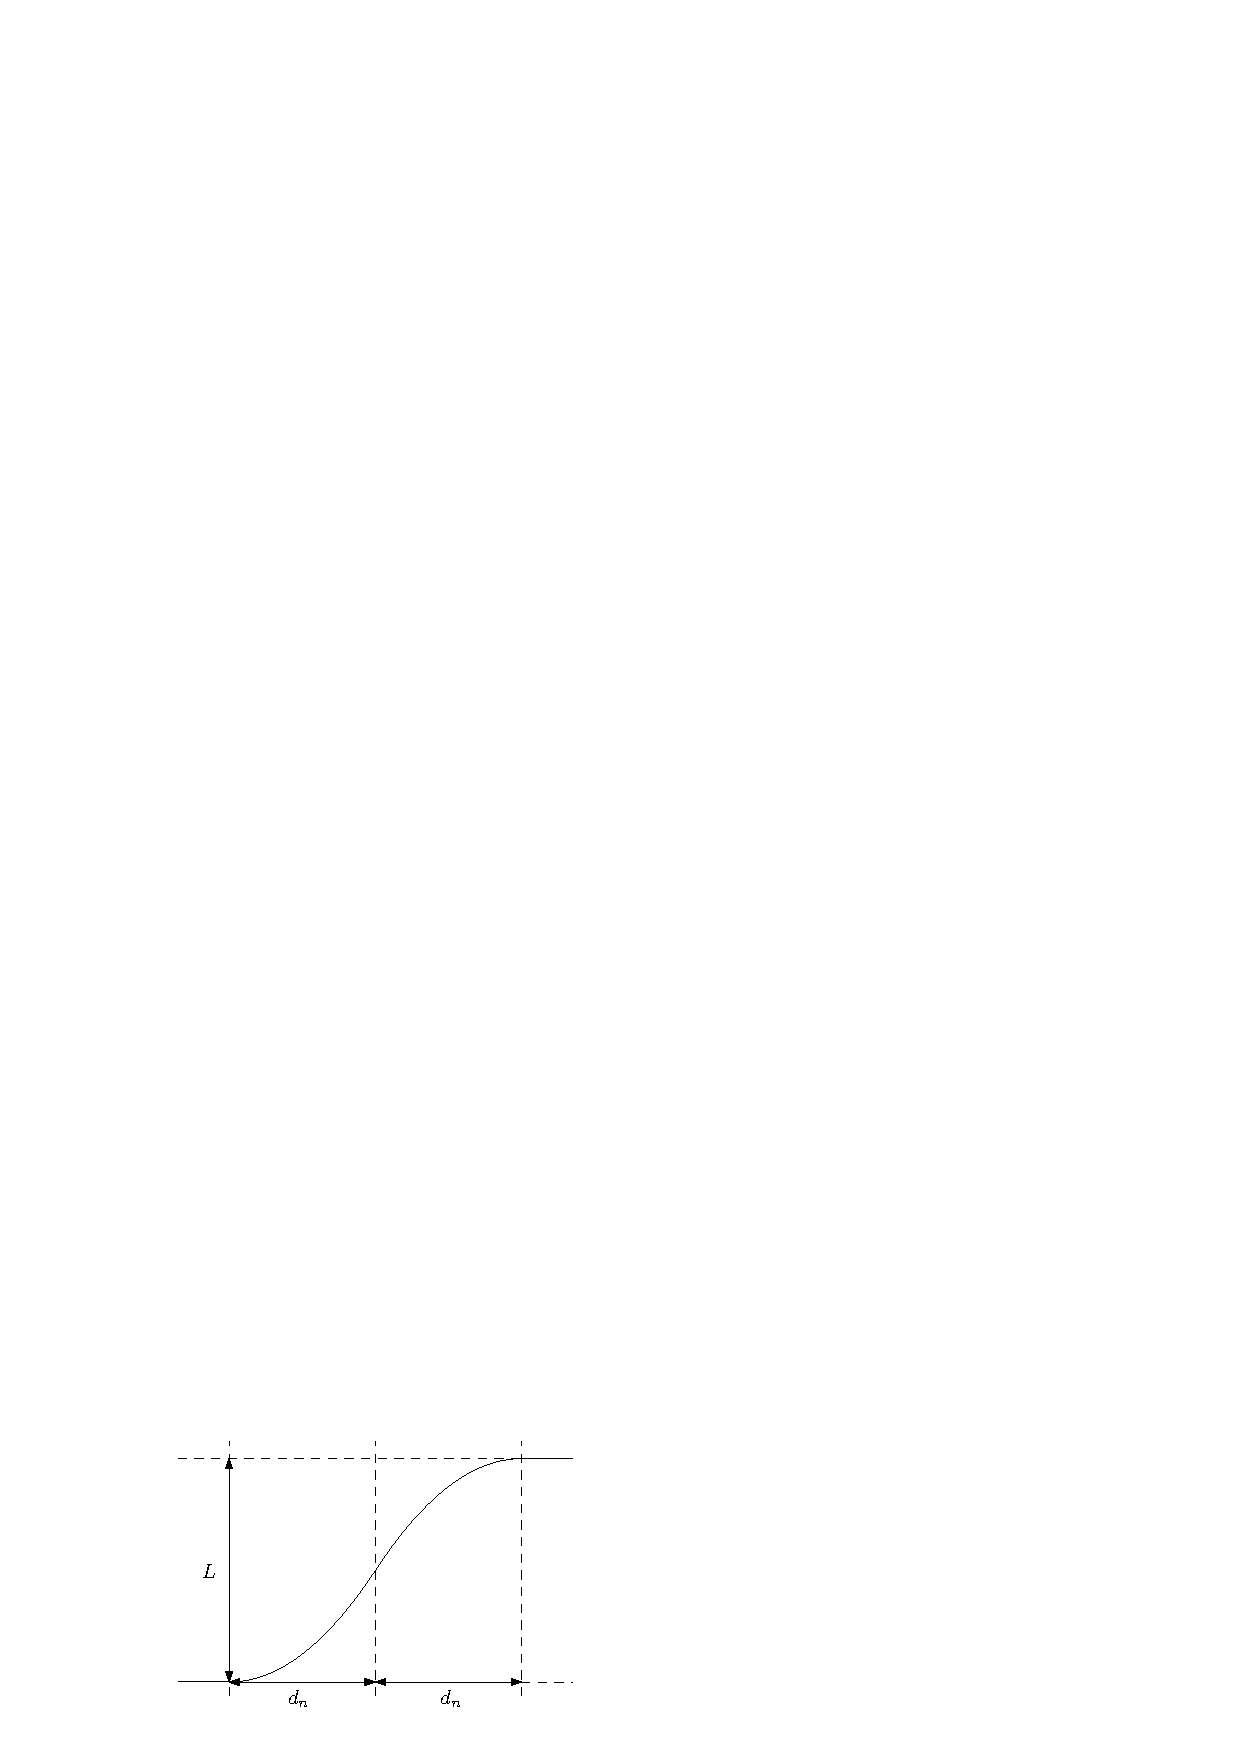
\includegraphics[scale=1.0]{figures/motion/start_stop_trajectory}
%   \caption{Shape of some start-stop trajectory of a single isolate vehicle
%     moving forward from some current waiting position $p_{k}$ to the next
%     $p_{k+1}$.}
%   \label{fig:start-stop}
% \end{figure}

% \begin{figure}
%   \centering
%   \includegraphics[width=0.99\textwidth]{figures/motion/merge}
%   \caption{Sketch how the initial deceleration merges with the first start-stop phase.}
%   \label{fig:merge}
% \end{figure}



% Finally, to simplify the upcoming analysis of optimal trajectories, we make the
% following assumption on lanes.

% \begin{assump}
%   Each lane has at least capacity for a single vehicle, so $c(v, w) \geq 1$,
%   or equivalently, the length of the lane must be at least
%   $d(v, w) \geq 2p^{+}(d_{f}) + W + L$, or in terms of the control problem
%   parameter $p_{0} \leq -2p^{+}(d_{f}) - L$.
% \end{assump}


\begin{figure}
  \centering
  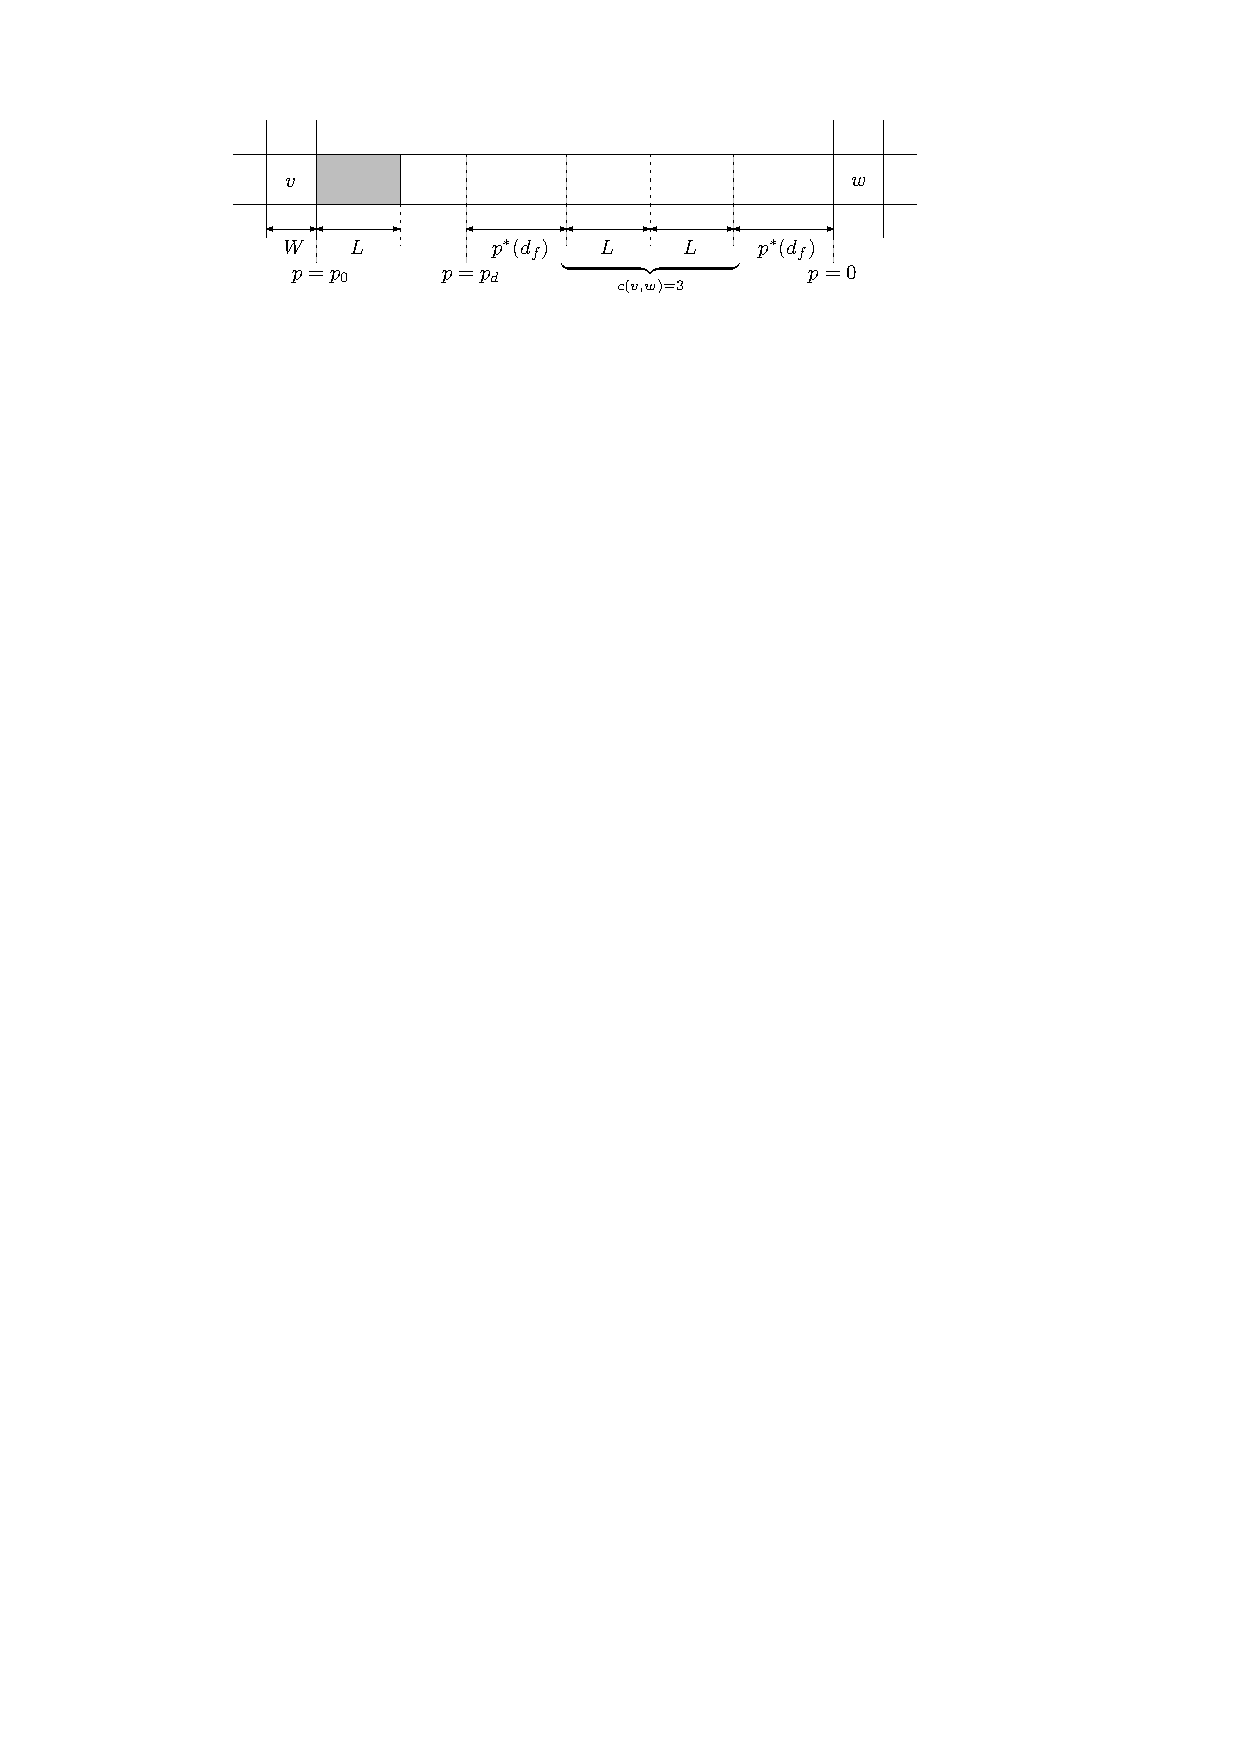
\includegraphics[width=0.99\textwidth]{figures/motion/tandem_annotated}
  \caption{Tandem of intersections with indicated distances used in the
    derivation of the stationary lane capacity, which is the maximum number of
    vehicles that can stop and wait in the lane, before they leave.}
  \label{fig:tandem_annotated}
\end{figure}


\newpage

\section{Vehicle scheduling in networks}

\begin{figure}
  \centering
  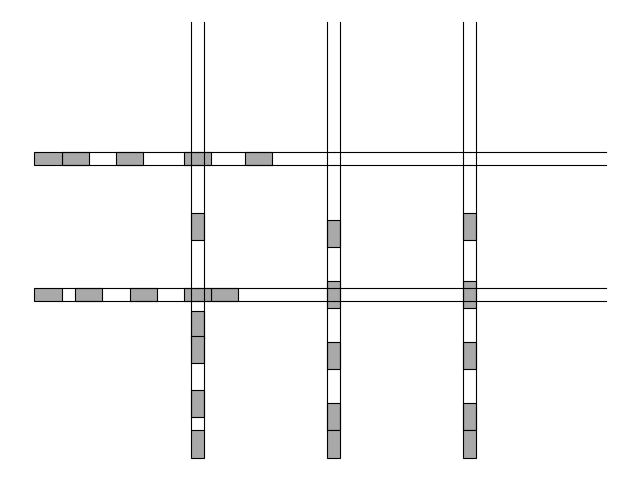
\includegraphics[width=0.55\textwidth]{figures/network/grid_example.png}
  \caption{Illustration of some grid-like network of intersections with vehicles
    drawn as grey rectangles. There are five vehicle routes: two from east to
    west and three from south to north. Turning at intersections is not
    allowed.}\label{fig:network_illustration}
\end{figure}

We now extend the single intersection model to a network of intersections
without turning routes, illustrated in Figure~\ref{fig:network_illustration}.
% network definition
We define a directed graph $(\bar{V},E)$ with nodes $\bar{V}$ and arcs $E$,
representing the possible paths that vehicles can follow. Nodes with only
outgoing arcs are \textit{entrypoints} and nodes with only incoming arcs are \textit{exitpoints}.
Let $V$ be the set of \textit{intersections}, which are all the nodes with
in-degree at least two.
%
Let $d(v, w)$ denote the distance between nodes $v$ and $w$.
%
For each route index $r \in \mathcal{R}$, we let
\begin{align*}
  \bar{V}_{r} = (v_{r}(0), v_{r}(1), \dots, v_{r}(m_{r}), v_{r}(m_{r}+1))
\end{align*}
be the path that vehicles $i \in \mathcal{N}_{r}$ follow through the network. We
require that the first node $v_{r}(0)$ is an entrypoint and that the last node
$v_{r}(m_{r}+1)$ is an exitpoint and we write
\begin{align*}
  V_{r} = \bar{V}_{r} \setminus \{ v_{r}(0), \, v_{r}(m_{r}+1) \}
\end{align*}
to denote the path restricted to intersections. We say that some $(v, w) \in E$
is on path $V_{r}$ whenever $v$ and $w$ are two consecutive nodes on the path
and we write $E_{r}$ to denote the set of all these edges. We require that
routes can only overlap at nodes by making the following assumption.

\begin{assump}\label{assump:disjoint_routes}
  Every arc $(v,w) \in E$ is part of at most one route $V_{r}$, such that routes
  do not share lanes. This ensures that the order of vehicles on each lane is
  completely determined by the order of vehicles on the corresponding lane.
\end{assump}

We start by considering networks in which all roads are axis-aligned such that
intersections always involve perpendicular lanes and where routes are such that
no turning is required. For each $v \in V_{r}$ define the conflict zone
$\mathcal{E}_{r}(v) = (b_{r}(v), e_{r}(v))$ and consider the union
\begin{align*}
  \mathcal{E}_{r} = \bigcup_{v \in V_{r}} \mathcal{E}_{r}(v)
\end{align*}
corresponding to the positions of vehicles $i \in \mathcal{N}_{r}$ for which it
occupies an intersection on its path $V_{r}$.
%
By reading $\mathcal{E}_{i} \equiv \mathcal{E}_{r}$ for $r(i) = r$, the single
intersection problem naturally extends to the network case. Like before, the
resulting problem can be numerically solved by a direct transcription method.

\subsection{General decomposition}
The general two-stage decomposition for the single intersection extends rather
naturally to the present model. Let for each pair $(i,v)$ of some vehicle
$i \in \mathcal{N}$ and an intersection $v \in V_{r(i)}$ along its route, let
\begin{align*}
\inf \{ t: x_{i}(t) \in \mathcal{E}_{r}(v) \} \;\; \text{ and } \; \sup \{ t: x_{i}(t) \in \mathcal{E}_{r}(v) \}
\end{align*}
be the crossing time and exit time, which we denote by $y(i,v)$ and
$y(i,v) + \sigma(i, v)$, respectively.
%
Instead of a single set of conflicts, we now define for each intersection
$v \in V$ in the network the set of conflict pairs
\begin{align*}
\mathcal{D}^{v} = \{ \{i,j\} \subset \mathcal{N} : r(i) \neq r(j), v \in V_{r(i)} \cap V_{r(j)} \} .
\end{align*}
Now the two-stage approach is to solve
\begin{align*}
  \min_{y,\sigma} \;\; & \sum_{r \in \mathcal{R}} F(y_{r}, \sigma_{r}) \\
  \text{ s.t. } & y(i,v) + \sigma(i,v) \leq y(j,v) \text{ or }  \\
                & y(j,v) + \sigma(j,v) \leq y(i,v) , & \text{ for all } \{i,j\} \in \mathcal{D}^{v} \text{ and } v \in V, \\
  & (y_{r}, \sigma_{r}) \in \mathcal{S}_{r} , \quad & \text{ for all } r \in \mathcal{R} ,
\end{align*}
%
where $F(y_{r}, \sigma_{r})$ and $\mathcal{S}_{r}$ are the value function and
set of feasible parameters, respectively, of the parametric trajectory
optimization problems
%
\begin{align*}
  F(y_{r}, \sigma_{r}) = \min_{x_{r}} & \; \sum_{i \in \mathcal{N}_{r}} J(x_{i}) \\
  \text{ s.t. } & x_{i}(t) \in D_{i}(s_{i,0}) , \quad & \text{ for } i \in \mathcal{N}_{r} , \\
  & x_{i}(y(i,v)) = b_{r}(v) , \quad & \text{ for } v \in V_{r} , i \in \mathcal{N}_{r} , \\
  & x_{i}(y(i,v) + \sigma(i,v)) = e_{r}(v) , \quad & \text{ for } v \in V_{r} , i \in \mathcal{N}_{r} , \\
  & x_{i}(t) - x_{j}(t) \geq L , \quad & \text{ for } (i, j) \in \mathcal{C} \cap \mathcal{N}_{r} ,
\end{align*}
where we again use subscript $r$ to group variables according to their associated route.


\subsection{Decomposition for delay objective}

Suppose we use use the crossing at the last intersection as performance measure, by defining the
objective function as
\begin{align*}
  J(x_{i}) = \inf \{ t: x_{i}(t) \in \mathcal{E}_{r}(v_{r}(m_{r}))\} .
\end{align*}
%
We show how to reduce the resulting problem to a scheduling problem, like we did
in the single intersection case.
%
We will again assume Assumption~\ref{assump:same_geometry} and
Assumption~\ref{assump:full_speed}, so vehicles will always cross intersections
at full speed, and all vehicles share the same geometry. Hence, the occupation
time $\sigma \equiv \sigma(i,v)$ is the same for all vehicles and intersections. For this
reason, we will write the shorthand $y_{r} \in \mathcal{S}_{r}$, because $\sigma_{r}$
is no longer a free variable.

As a consequence of Assumption~\ref{assump:same_geometry} and Assumption~\ref{assump:full_speed},
each lower-level trajectory optimization problem for a given route
$r \in \mathcal{R}$ decomposes into a sequence of problems, each corresponding to
two consecutive intersection along $V_{r}$.
%
This means that $y_{r} \in \mathcal{S}_{r}$ is equivalent to
$y_{(v,w)} \in \mathcal{S}_{(v,w)}$ for each $(v,w) \in E_{r}$, where
$y_{(v,w)}$ denotes the vector of all variables $y(i, v)$ and $y(i, w)$ for all
$i \in \mathcal{N}_{r}$ and $\mathcal{S}_{(v,w)}$ denotes the set of values of $y_{(v,w)}$ for which a feasible trajectory part can be found.
%
Hence, we will now focus on a tandem of two intersections and investigate the
trajectories of vehicles in this with the goal of stating sufficient conditions
for $y_{(v,w)} \in \mathcal{S}_{(v,w)}$.

\subsection{Crossing time scheduling}

%The Job-Shop Scheduling Problem (JSSP) is a widely studied problem in which a
%set of $n$ jobs must be assigned to non-overlapping time slots on a set of $m$
%machines. Each job $i$ has a set of $n_{i}$ operations
%$O_{i1}, \dots, O_{in_{i}}$ that need to be executed in this order. Each
%operation $O_{ij}$ requires $p_{ij}$ processing time on machine $M_{ij}$. Each
%machine can process at most one operation and early preemption is not allowed.
%The task of the scheduler is to determine a valid schedule of start times
%$y_{ij}$ for each operation, while minimizing some objective function. Let
%$C_{ij} = y_{ij} + p_{ij}$ denote the \textit{completion time} of operation
%$O_{ij}$, then the \textit{makespan} objective is given by the latest completion
%time $\max_{i,j} C_{ij}$. Another objective is the \textit{total completion
%  time}, given by
%\begin{align*}
%  \sum_{i=1}^{n} \sum_{j=1}^{m} C_{ij} ,
%\end{align*}
%which may be intuitively be thought of as representing some sort of total cost
%of inventory, assuming we need to physically store jobs somewhere.
%
%A commonly used representation of JSSP instances is the \textit{disjunctive
%  graph} $G = (\mathcal{O}, \mathcal{C}, \mathcal{D})$, with vertices
%$\mathcal{O} = \{ O_{ik} : 1 \leq i \leq n, 1 \leq k \leq n_{i} \}$
%corresponding all the operations. The set of \textit{conjunctive arcs}
%$\mathcal{C}$ encodes all the precedence constraints
%$O_{i,k} \rightarrow O_{i,k+1} $ among each job's operations. The set of
%\textit{disjunctive edges} $\mathcal{D}$ consists of undirected edges between
%each pair of operations from distinct jobs that need to be processed on the same
%machine, effectively encoding all such \textit{conflicts}. Each valid schedule
%induces an ordering of operations on machines that is encoded by fixing the
%direction of each disjunctive edge such that we obtain a direct acyclic graph.
%
%\begin{itemize}
%  \renewcommand\labelitemi{--}
%{\color{gray}
%% job-shop disjunctive graph
%\item Introduce general job-shop problem and disjunctive graph, see Figure~\ref{fig:disjunctive_graph}.
%% define travel constraints
%\item Introduce travel constraints and its disjunctive graph arcs.
%% define buffer constraints
%\item Introduce buffer constraints and its disjunctive graph arcs.
%
%% branch-and-bound
%\item Formulate MILP problem and investigate how the solving time scales with network
%size in terms of number of intersections and number of vehicles in the network.
%Do the single intersection cutting planes still hold? Are there any obvious
%cutting planes?
%}
%\end{itemize}
%
%Let $y(i,v)$ denote the crossing time of vehicle $i$ at intersection $v \in V$.
%Let $\mathcal{C}$ be the conjunctive pairs and let $\mathcal{D}^{v}$ denote the
%disjunctive pairs at intersection $v \in V$.
%%
%Writing $\texttt{conj(\dots)}$ and $\texttt{disj}(\dots)$ for the usual
%conjunctive and disjunctive constraints, we propose to solve the optimization
%problem
%\begin{subequations}\label{eq:network_problem}
%\begin{align}
%  \min_{y} \quad & \sum_{i \in \mathcal{N}} \sum_{v \in \mathcal{R}(l(i))} y(i,v) & \\
%  \text{s.t.} \quad & r_{i} \leq y(i, v_{0}(l(i))) & \text{ for } i \in \mathcal{N} , \\
%  & \texttt{conj}(y(i,v), y(j,v)) & \text{ for } (i,j) \in \mathcal{C}, v \in V , \\
%  & \texttt{disj}(y(i,v), y(j,v)) & \text{ for } \{i,j\} \in \mathcal{D}^{v}, v \in V , \\
%  & y(i, v) + d(v, w) \leq y(i, w) & \text{ for } i \in \mathcal{N}(l), (l, v, w) \in E, \label{eq:travel_delay} \\
%  & y(i, w) + \rho(v, w) \leq y(j, v) & \text{ for } (i,j,v,w) \in \mathcal{F} , \label{eq:buffer_constraints}
%\end{align}
%\end{subequations}
%where $\mathcal{F}$ is defined as
%\begin{align*}
%  \mathcal{F} = \{ (i,j,v,w) : i,j \in \mathcal{N}(l), k(i) + c(v,w) = k(j),  (l,v,w) \in E\}
%\end{align*}
%and we have $\rho(v, w) = c(v, w) L - d(v, w)$. Each $(i,j,v,w) \in \mathcal{F}$
%represents a pair of vehicles driving on the same lane $(v,w)$, for which the
%first vehicle must have made enough space in the lane before vehicle $j$ can
%enter.


Analogously to the single intersection case, we let the earliest crossing time
$\beta_{t}(i, v)$ for vehicle $i = (r,k) \in \mathcal{N}$ at network nodes
$v \in \bar{V}_{r}$ in current disjunctive graph $G_{t}$ be recursively
defined through
\begin{align*}
  \beta_{t}(i, v) =
  \begin{cases}
  a(i, v) & \text{ if $v$ is an entrypoint}, \\
  \max_{i \in \mathcal{N}_{t}^{-}(j)} \beta_{t}(i, v) + w(i, j) & \text{ otherwise},
  \end{cases}
\end{align*}
where $\mathcal{N}_{t}^{-}(j)$ is again the set of in-neighbors of node $j$ in
$G_{t}$.
%
For empty schedules, it is easily seen that we have
$\beta_{0}(i, v_{r}(0)) = a(i, v_{r}(0))$ for entrypoints and we have
$\beta_{0}(i, v_{r}(l + 1)) = \beta_{0}(i, v_{r}(l)) + d(v_{r}(l), v_{r}(l+1)) / v_{\max}$
for $l=1,\dots, m_{r}$, so between consecutive intersections on the same route.

There are two natural choices for the objective to optimize in this scheduling
setting.
%
We minimize the time each vehicle is in the system, which is equivalent to
minimizing the delay at the last intersection of each vehicle's route, written as
\begin{align*}
  \text{obj}_{1}(y) = \sum_{i \in \mathcal{N}} y(i, v_{r}(m_{r})) - \beta_{0}(i, v_{r}(m_{r})) .
\end{align*}
Alternatively, it also makes sense to minimize the delay at every
intersection along each vehicle's route, so we can also minimize
\begin{align*}
  \text{obj}_{2}(y) = \sum_{i \in \mathcal{N}} \sum_{v \in V_{r(i)}} y(i, v) - \beta_{0}(i, v) .
\end{align*}


%\begin{figure}
%  \centering
%  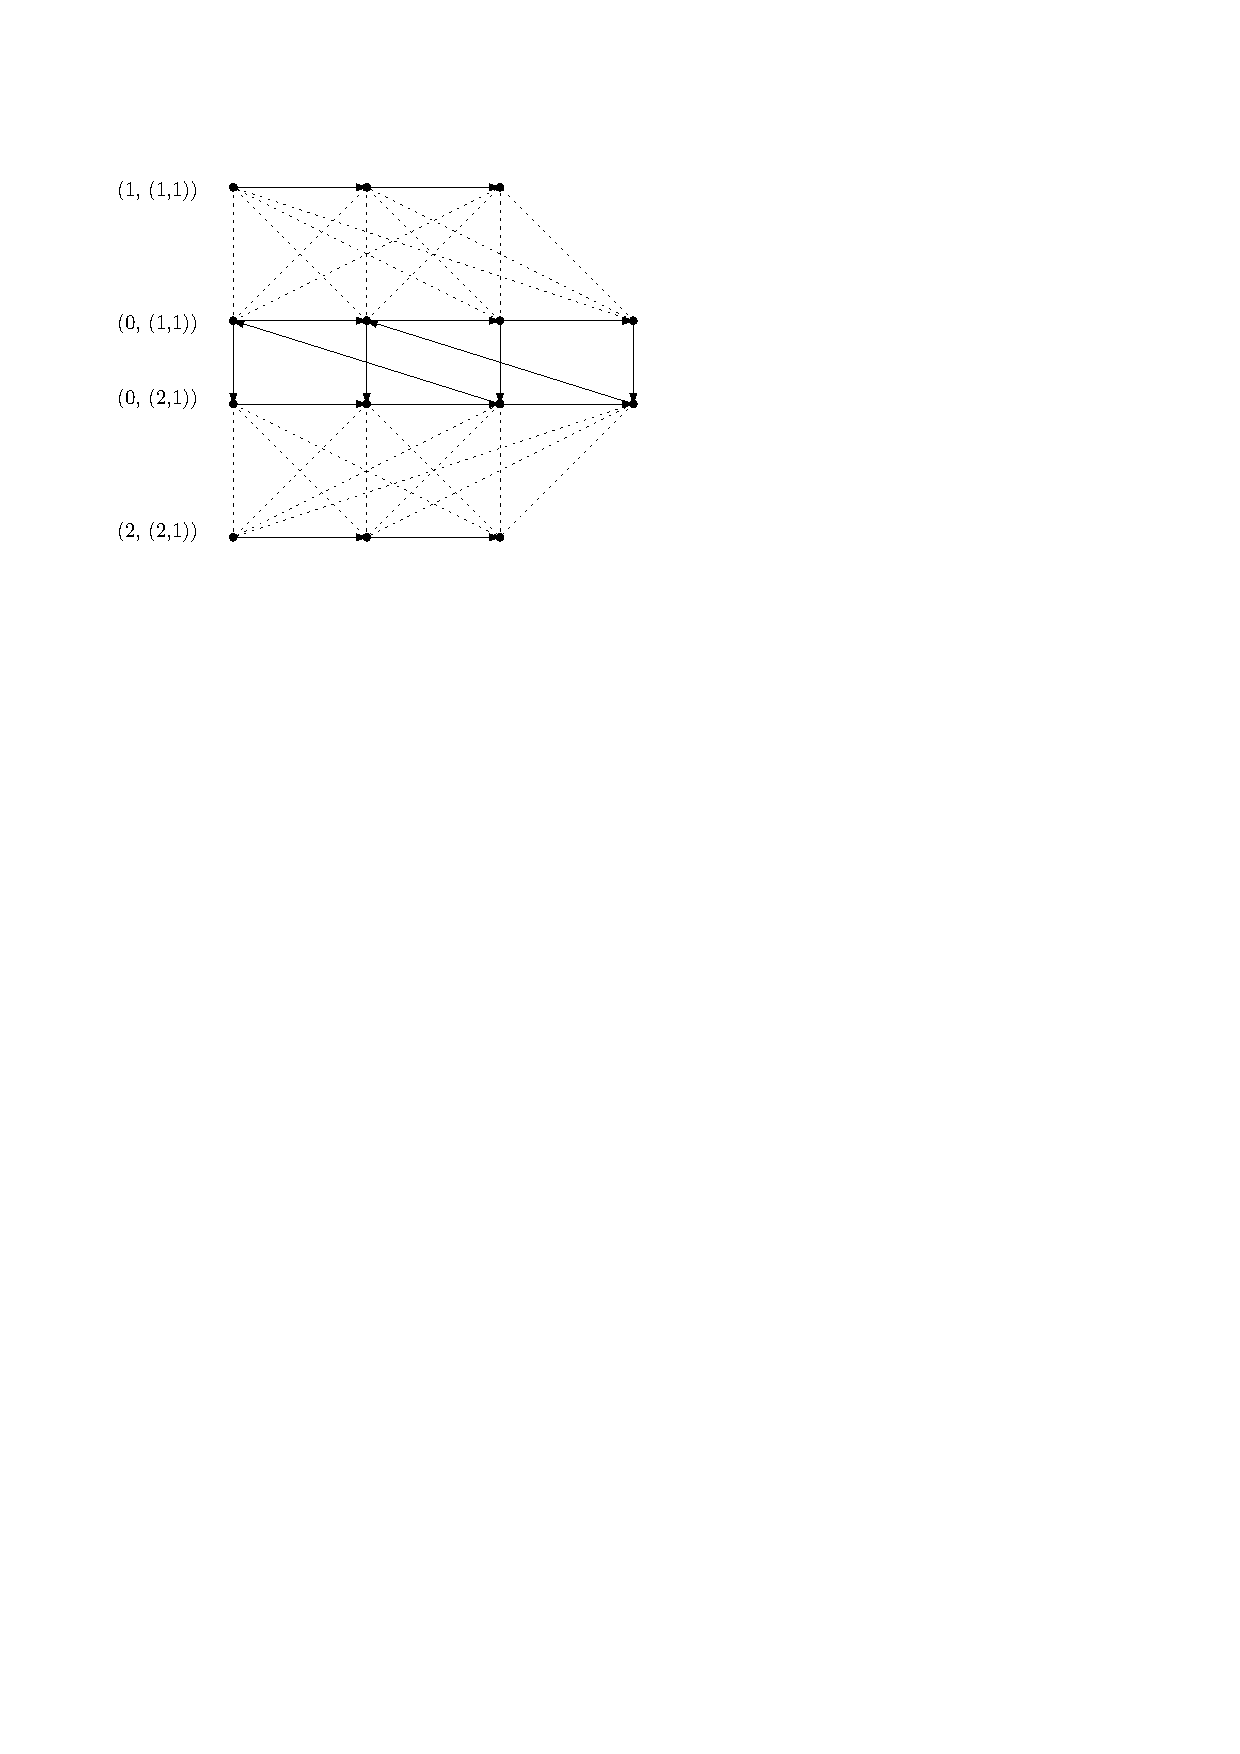
\includegraphics[scale=1]{figures/network/disjunctive_graph}
%  \caption{Empty disjunctive graph belonging to a tandem of two intersections,
%    labeled $v$ and $w$. There are three routes $\mathcal{R} = \{0, 1, 2\}$. On
%    route 0, four vehicle are arriving, the other two routes have 3 arrivals
%    each. Conjunctive arcs are drawn as from left to right, travel arcs are
%    drawn from top to bottom and disjunctive arcs are drawn as dotted lines. Two
%    buffer constraints are drawn as diagonal arcs, corresponding to a capacity
%    of 2 vehicles for the lane between both intersections.}
%  \label{fig:disjunctive_graph}
%\end{figure}

\newpage
\section{Learning to schedule}

Like in the single intersection case, we try to model optimal solutions using
autoregressive models.
%
In the single intersection case, we argued that each schedule is uniquely
defined by its route order $\eta$. Generalizing this to the case of multiple
intersections, we see that a schedule is uniquely defined by the set of route
orders $\eta^{v}$ at each intersection $v \in V$. Instead of working with such a set
of sequences, we will intertwine these sequences to obtain a single \textit{crossing sequence}
$\eta$, which consists of pairs $(r, v)$ of a route $r \in \mathcal{R}$ at some
intersection $v \in V_{r}$ and we will refer to such a pair as a \textit{crossing}. Of
course, this crossing sequence can be constructed in many different ways,
because it does not matter in which order the intersections are considered,
which is illustrated in Figure~\ref{fig:solution_equivalence}.
% \begin{align*}
%   | \{ t : \nu_{t} = v \} | = |\eta^{v}| \quad \text{ for each } v \in V ,
% \end{align*}
Given some problem instance $s$, we will consider autoregressive models of the form
\begin{align}
  \label{eq:autoregressive}
  p(\eta | s) =  \prod_{t=1}^{N} p(\eta_{t}| s, \eta_{1:t-1}) .
\end{align}

These models can also be understood in terms of a step-by-step schedule
construction process that transitions from a partial schedule state
$s_{t} = (s, \eta_{1:t})$ to the next state $s_{t+1}$ by selecting some \textit{action}
$\eta_{t+1} = (r_{t+1}, v_{t+1})$. We say a crossing is pending when it still has
unscheduled vehicles. Similarly, we say an intersection is pending when some of
its crossings are still pending. With these definitions, the set of \textit{valid actions}
$\mathcal{A}(s_{t})$ at some intermediate state $s_{t}$ is exactly the set of
pending crossings.
%
% multiple correct actions
We again emphasize that multiple sequences of actions lead to the same schedule,
because the order in which intersections are considered does not matter for the
final schedule, which is illustrated in Figure~\ref{fig:solution_equivalence}.
%
The models that we study can be understood as being parameterized as some
function of the disjunctive graph $G_{t}$ of partial schedule $s_{t}$, so an
alternative way of writing~\eqref{eq:autoregressive} that emphasizes this is
\begin{align}
  p(\eta = ((r_{1}, v_{1}), \dots, (r_{N}, v_{N})) \; | \; s) = \prod_{t=1}^{N} p(r_{t}, v_{t} | G_{t-1}) .
\end{align}
%
Instead of modeling the joint
probability distribution $p(r_{t}, v_{t} | G_{t-1})$ over crossings, we can also apply
the chain rule to factorize it as
\begin{align}
  p(r_{t}, v_{t} | G_{t-1}) = p(r_{t} | v_{t} , G_{t-1}) p (v_{t} | G_{t-1}) .
\end{align}
In this case, the model $p(r_{t} | v_{t}, G_{t-1})$ can be thought of as
predicting a set of actions, one for each intersection.

\begin{figure}
  \centering
  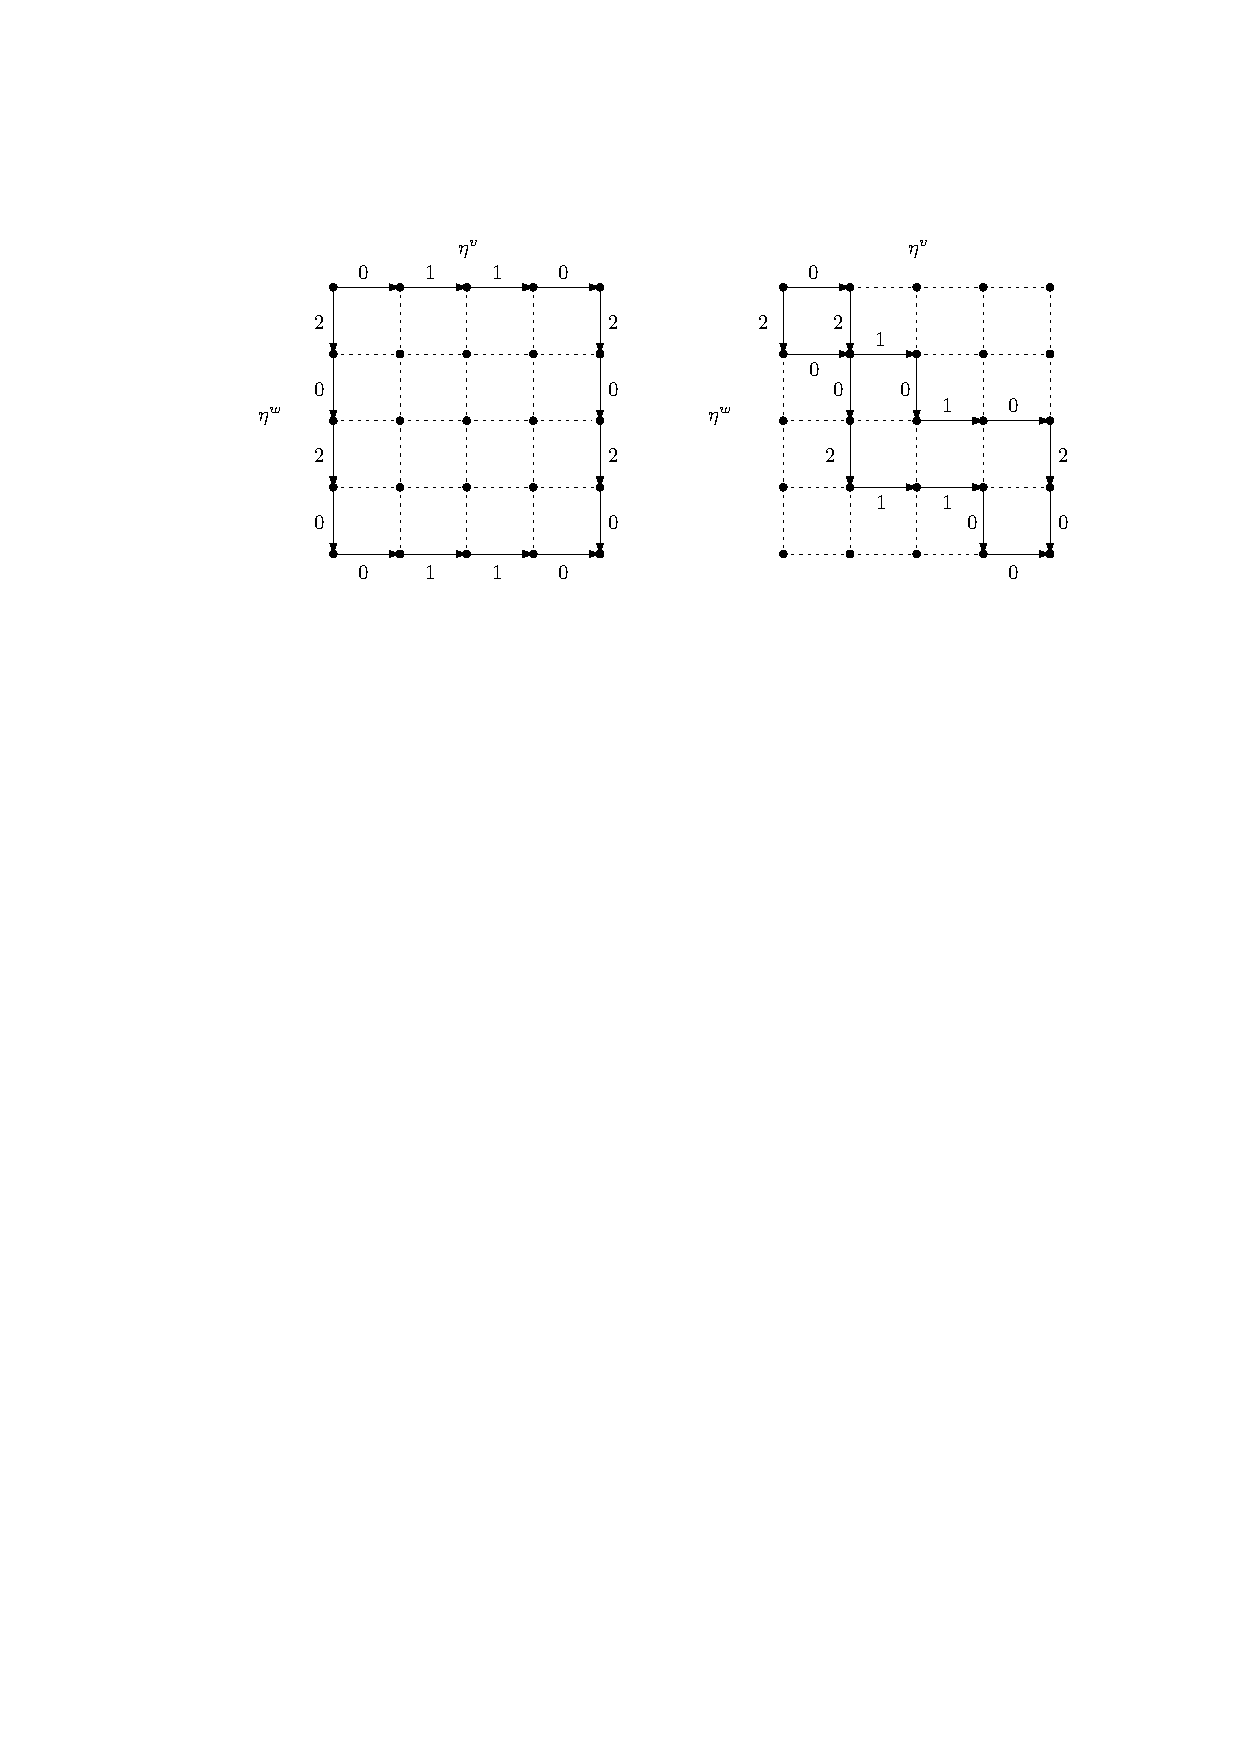
\includegraphics[width=0.9\textwidth]{figures/network/solution_equivalence}
  \caption{When each route order is locally fixed at every intersection, the
    global crossing sequence is not uniquely determined, because these local
    sequences may be merged in any order. Suppose we have a tandem of two
    intersections and a horizontal arrows correspond to taking the next local
    action at intersection $v$, a vertical arrows correspond to taking next
    local action at intersection $w$. Each valid crossing sequence corresponds
    to some path from the top-left to the bottom-right corner. Although any such
    crossing sequence produces the same schedule, it might be that our
    autoregressive model fits better on some sequences than others. For example,
    we might expect that sequences on the boundary of the grid, shown in the
    left grid, are harder to learn from data than sequences that stay closer to
    the diagonal, like in the right grid. The intuition is that we need to
    ``look into the future'' more to learn the former, while in the latter
    trajectories, progress in the two intersections is more balanced.}
  \label{fig:solution_equivalence}
\end{figure}

\paragraph{Intersection visit order.}
In the general class of autoregressive models for inputs and outputs with sets,
of which our model above is a special case (we have a set of sequences as
output), it has been noted before that the order in which inputs or outputs are
presented to the model during training has a considerable impact on the final
model fit~\cite{vinyalsOrderMattersSequence2016}.
%
For our model, we also expect to find this effect, so we will investigate the
impact of the order in which intersections are visited, determined by
$p(v_{t} | G_{t-1})$. We now propose some heuristic ways to define
$p(v_{t} | G_{t-1})$. Later, we will consider a neural network parameterization.
% random
First of all, the simple \textit{random} strategy would be to sample some
intersection with pending crossings at each step.
% ``boundary'' (or ``exhaustive'')
In the \textit{boundary} strategy, we keep visiting the same intersection until
it is done (when it has no pending crossings anymore), then move to some next
intersection. When the network of intersections is free of cycles, we could for
example follow some topological order. We use the term ``boundary'' because this
strategy produces trajectories along the boundary of the grid in
Figure~\ref{fig:solution_equivalence}.
% ``alternate''
In the \textit{alternating} strategy, we keep alternating between intersection to keep
the number of scheduled vehicles balanced among them. This produces trajectories
that can be understood as being close to the ``diagonal'' of the grid in
Figure~\ref{fig:solution_equivalence}. Again, the order in which we alternate between intersections may
again be based on some topological order.


\subsection{Model parameterization}

\subsubsection{Threshold heuristics}
It is straightforward to extend the threshold rule to networks of
intersections, when assuming a fixed intersection order. Each time some
next intersection is visited, we apply the single intersection threshold rule to
pick the next route. This is straightforward to do, because we can just consider
the disjunctive subgraph induced by the nodes belonging to that intersection to
arrive at the single intersection case.
%
Furthermore, the definition of the threshold rule itself does not depend on the
network of intersections. This is a desirable property, because it allows us to
tune the threshold on small networks and then apply it on larger ones.


\subsubsection{Neural constructive heuristic}
\label{sec:neural_constructive}

We will now propose a neural network parameterization of
$p(r_{t} | v_{t}, G_{t-1})$ and train it based on optimal schedules in a
supervised learning setting. The model can be best understood as solving a
so-called multi-label classification problem, because it needs to provide a
distribution over routes at every intersection.
%
The training data set $\mathcal{X}$ consists of pairs
$(G_{t-1}, (r_{t}, v_{t}))$, to which we refer to as \textit{state-action} pairs
to draw the parallel with the terminology used in the reinforcement learning
literature.
%
To obtain these pairs, we sample a collection of problem instances, which are
solved to optimality using a MILP solver. For each optimal schedule, we compute
the corresponding optimal route order $\eta^{v}$ for each intersection.
%
From these, we can construct $\mathcal{X}$ in different ways.
% sample a single intersection order for each instance
For example, for each solved instance, we can randomly select some intersection
order $\mu$, which fixes the crossing order $\eta$. We can then replay
this sequence of actions step-by-step to obtain the corresponding sequence of
state-action pairs.
% multiple intersection order per instance
The model might become more robust when training on multiple samples of
intersections orders per instance.
% fixed intersection order
Alternatively, we can consider one of the fixed intersection orders
described at the start of this section (random, boundary, alternating).
% lookahead
Furthermore, combined with one of the above strategies, we can also employ some
kind of fixed lookahead procedure, as illustrated in
Figure~\ref{fig:state_action_collection}.
% inference
At inference time, we use the same intersection order as during training and at
each step we greedily select $r_{t}$.

%\begin{figure}
%  \centering
%  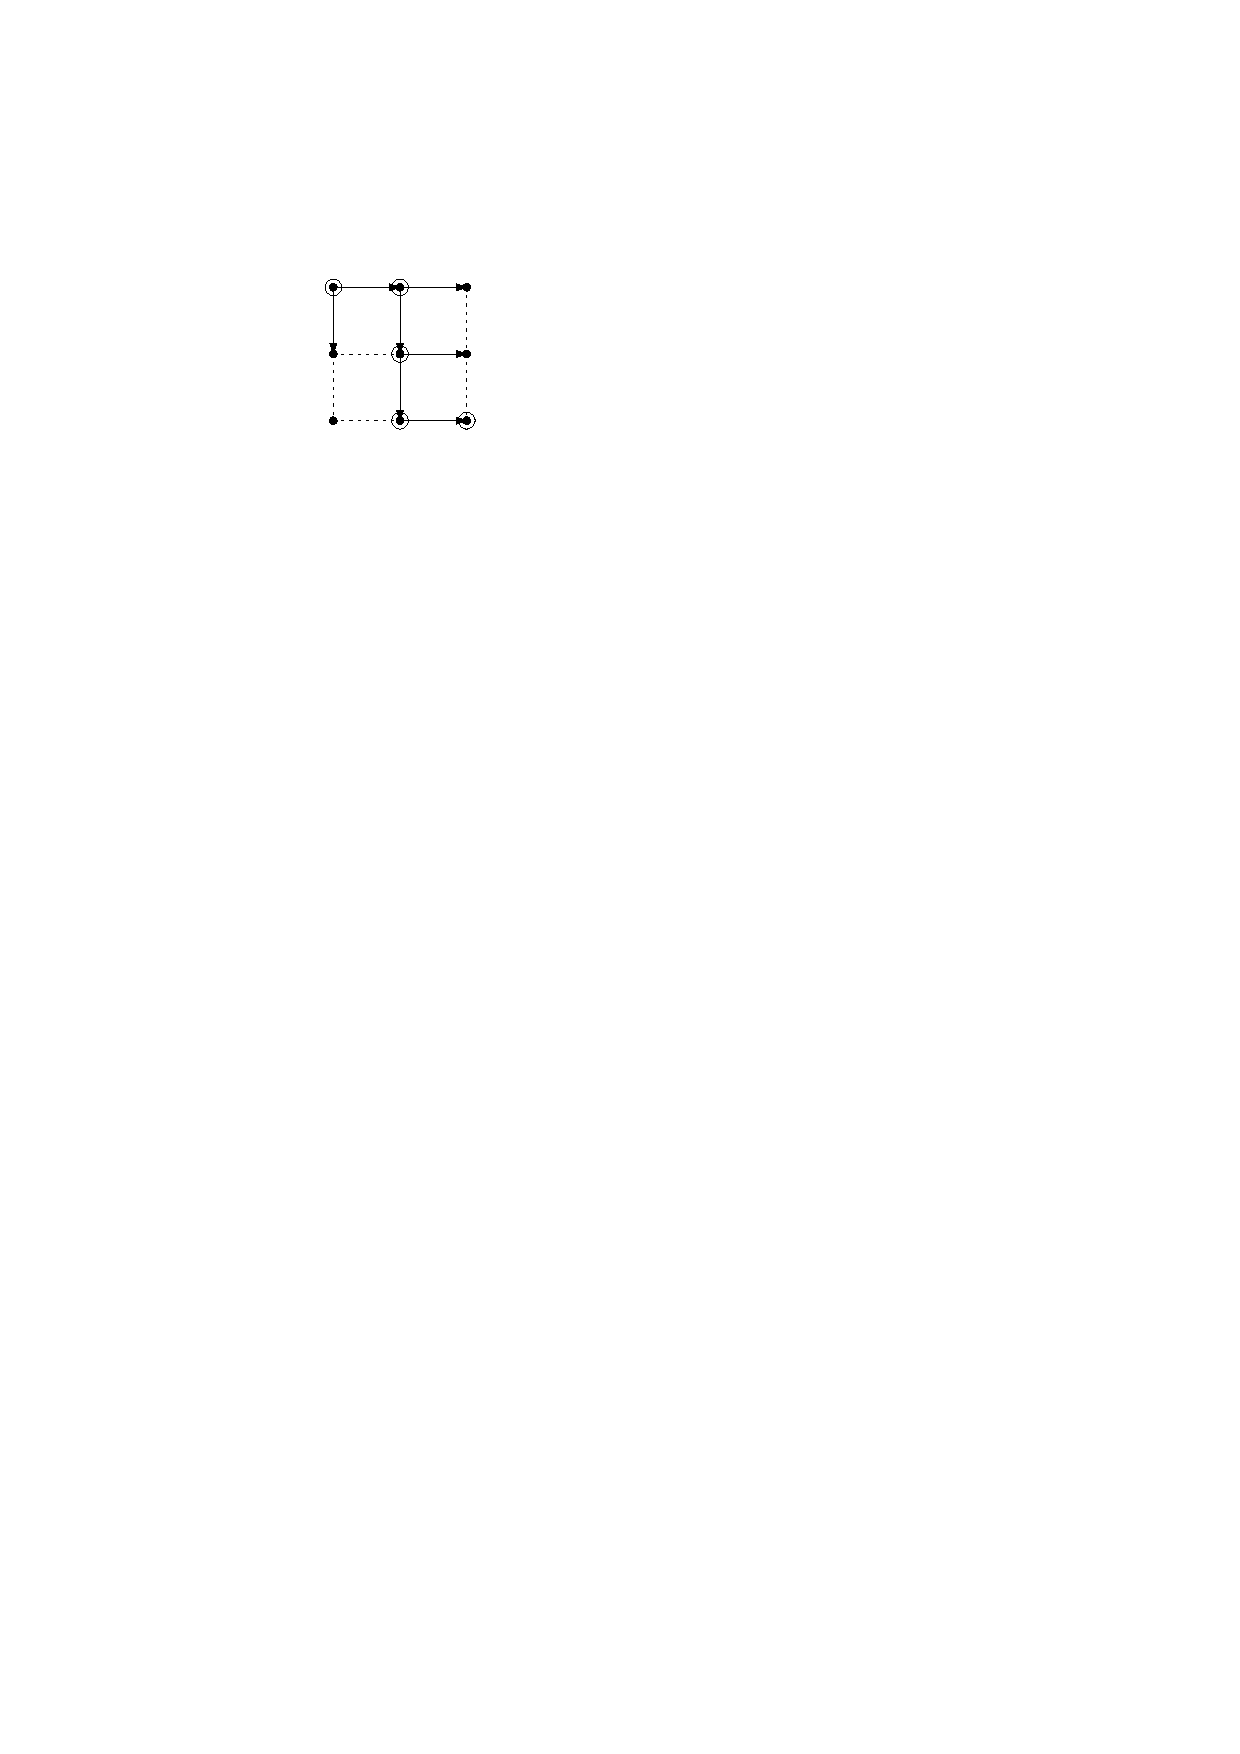
\includegraphics[scale=1.2]{figures/network/state_action_collection}
%  \caption{Possible strategy for collecting state-action pairs: one action
%    look-ahead. At every state $s_{t}$ with a set of possible actions
%    $\mathcal{A}(s_{t})$, we add all state-action pairs
%    $\{ (s, a) : a \in \mathcal{A}(s) \}$, but we pick a single action $a^{*}$
%    to move to the next state. In the figure, the state-action pairs are
%    depicted as solid arrows. The encircled dots are the states that are
%    actually visited. Observe that this procedure can be naturally generalized
%    to a look-ahead of arbitrary depth.}
%  \label{fig:state_action_collection}
%\end{figure}

We will now describe how the model is parameterized based on recurrent
embeddings of the sequences of crossing time lower bounds at each crossing, in a
somewhat similarly to how we used the horizons in the single intersection model.
%
Let $k(r, v)$ denote the number of scheduled vehicles at crossing $(r, v)$ and
let $n_{r}$ denote the total number of vehicles on route $r$. For each crossing
$(r, v)$, consider the earliest crossing time of the next unscheduled vehicle,
which we denote as
\begin{align*}
  T(r, v) = \beta(r, k(r, v) + 1, v) .
\end{align*}
We define the \textit{horizon} of crossing $(r, v)$ to be the sequence of relative lower bounds
\begin{align*}
  h(r, v) = (\beta(r, k(r, v) + 2, v) - T, \dots, \beta(r, n_{r}, v) - T) .
\end{align*}
%
Each such horizon is embedded using an Elman RNN. To produce a logit for each
crossing, these embeddings are fed through a feedforward network, consisting of
two hidden layers of size 128 and 64 neurons with relu activation and batch
normalization layers in between. See Figure~\ref{fig:rnn_model} for a schematic
overview of the architecture. {\color{Navy} Next: instead of $h(r, v)$, feed
  $(T(r, v), h(r, v))$ to the FF.}

%\begin{figure}
%  \centering
%  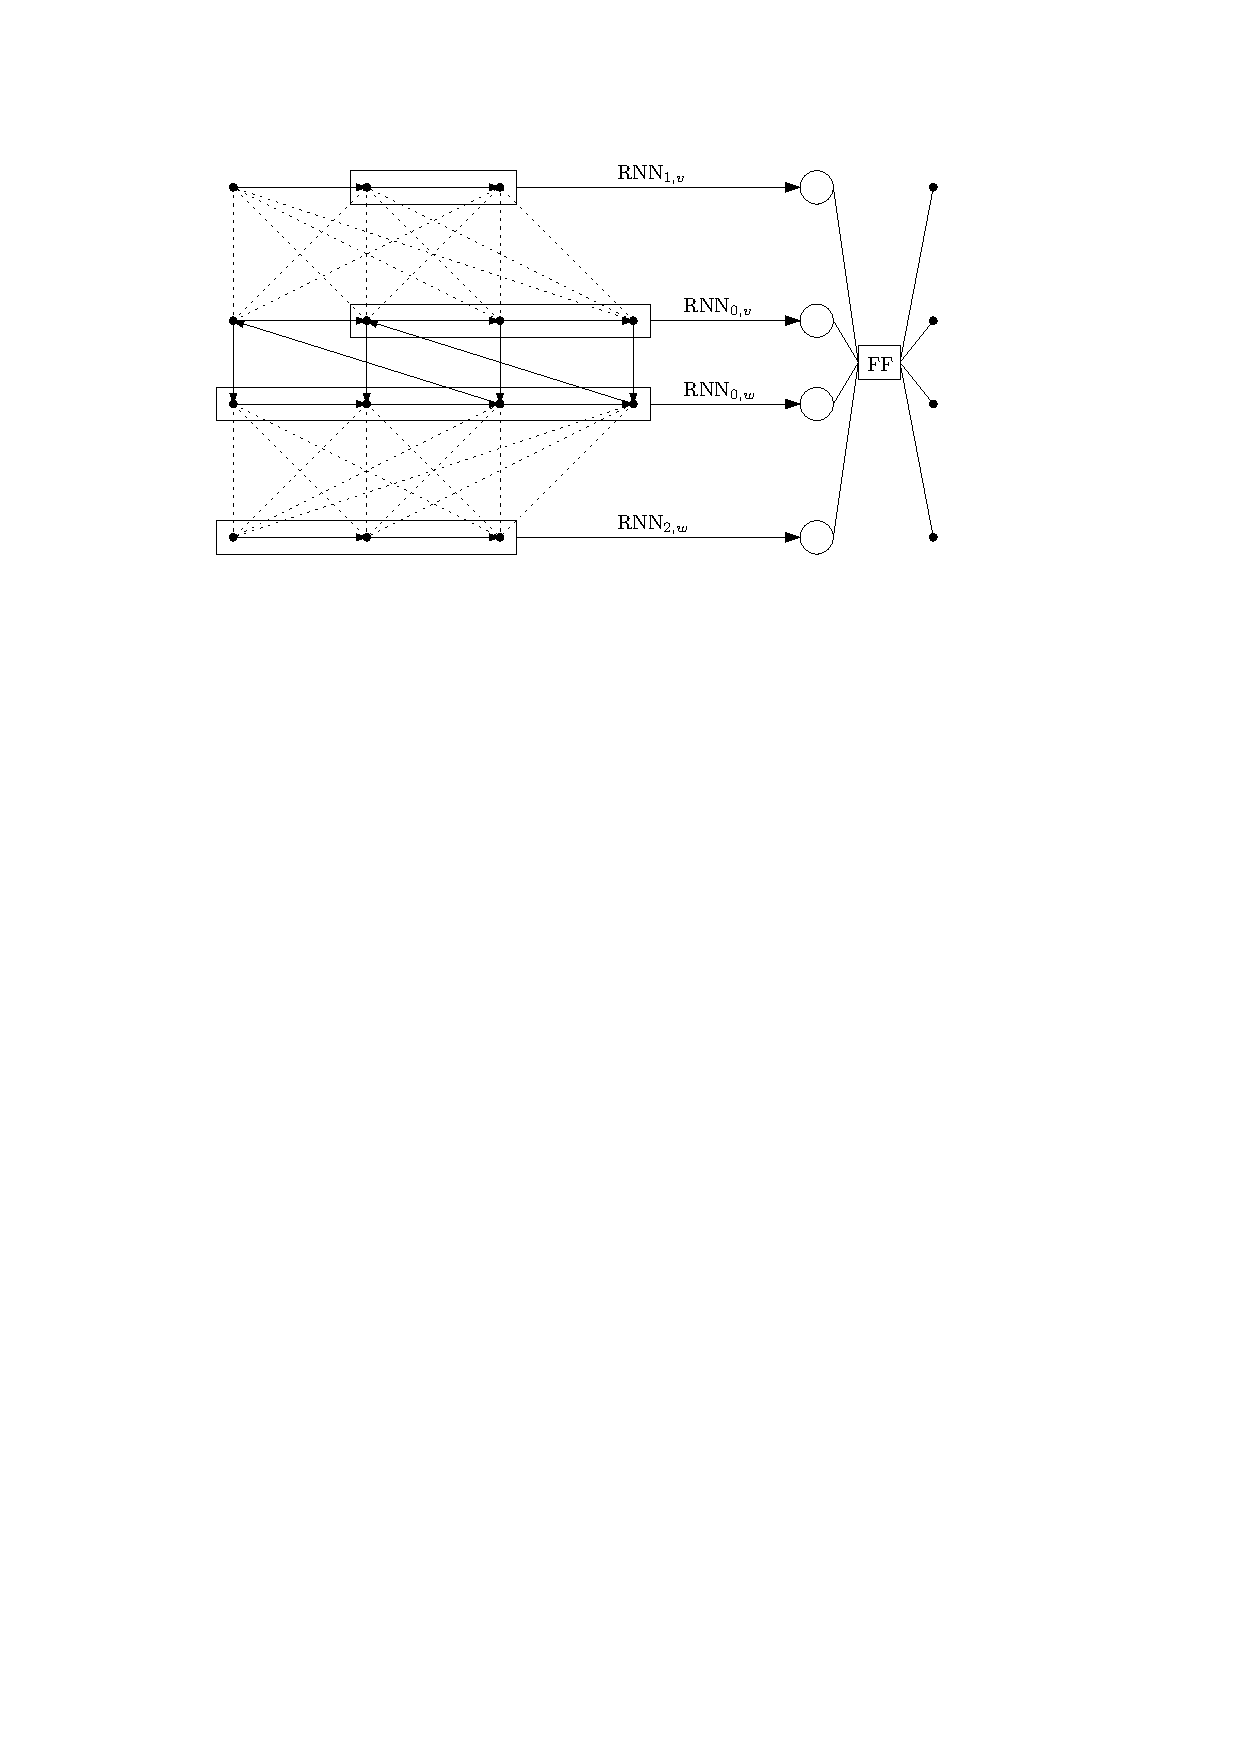
\includegraphics[scale=1]{figures/network/rnn_model}
%  \caption{Illustration of model with RNN encoding of horizon at each crossing.
%    The disjunctive graph nodes whose lower bounds are part of the current
%    horizons are indicated with rectangles. The RNN embeddings (open circles)
%    are fed through a final feedforward network to produce a logit (dots) for
%    each crossing.}
%  \label{fig:rnn_model}
%\end{figure}

To train the model, we use the Adam optimizer with learning rate~$10^{-4}$ and a
batch size of $40$ state-action pairs. We experienced a case of the exploding
gradients problem when we did not use the batch normalization layers. To allow a fair comparison of methods accross instances of different
sizes, both in terms of the number of vehicles and the size of the network, we
adapt both objective as follows.
% objective variant 1
For the first variant, we divide by the total number of vehicles, so we report
$\text{obj}_{1}(y) / |\mathcal{N}|$. Given some problem instance, let $N$ denote
the length of a crossing sequence, so it is also the total number of
vehicle-intersection pairs $(i, v)$ that need to be scheduled. For the second
objective variant, we consider the average delay per vehicle-intersection pair,
so we report $\text{obj}_{2}(y) / N$, which we report in Table~\ref{tab:results}.

% silent package loading


\begin{knitrout}
\definecolor{shadecolor}{rgb}{0.969, 0.969, 0.969}\color{fgcolor}\begin{table}
\centering
\caption{\label{tab:results}Average scaled optimal objective value computed using MILP and using the threshold heuristic with threshold $\tau = 0$. Each class of problem instances is identified by the number $n$ of vehicle arrivals per route and the grid network size as cols x rows.}
\centering
\resizebox{\ifdim\width>\linewidth\linewidth\else\width\fi}{!}{
\begin{tabular}[t]{cc|cc|c|c|c|ccc|cc|c|c|c|ccc|cc|c|c|c|ccc|cc|c|c|c|ccc|cc|c|c|c|ccc|cc|c|c|c|ccc|cc|c|c|c|ccc|cc|c|c|c|c}
\toprule
n & size & MILP & time & $\tau = 0$  (gap) & random (gap) & boundary (gap) & alternate (gap)\\
\midrule
5 & 2x1 & 57.27 & 0.06 & 65.27 (11.45\%) & 58.96 (2.95\%) & 58.72 (2.52\%) & 58.23 (1.66\%)\\
5 & 3x1 & 57.67 & 0.12 & 68.34 (15.44\%) & 59.77 (3.65\%) & 59.82 (3.74\%) & 58.72 (1.83\%)\\
5 & 3x2 & 57.35 & 1.38 & 69.17 (18.32\%) & 60.88 (6.16\%) & 60.36 (5.25\%) & 58.82 (2.56\%)\\
\bottomrule
\end{tabular}}
\end{table}

\end{knitrout}



\subsection{Reinforcement learning}

Instead of using a fixed training set $\mathcal{X}$ of state-action pairs during
training, we can fit our model from the perspective of a reinforcement learning
problem, which we already alluded to in Section~\ref{sec:neural_constructive}.
%
More precisely, given some scheduling problem instance $s$, we are dealing with
a Deterministic Markov Decision Process (DMDP), where partial disjunctive graphs
serve as states and crossings correspond to actions.
%
The potential benefit of using reinforcement learning is that we do not have to
fix an intersection order: our hope is that the training procedure will
automatically converge to some good intersection order.

{\color{Navy} The threshold heuristic ($\tau = 0$) can provide a
  \textit{baseline} for reinforcement learning, reducing the variance of the
  REINFORCE estimator.}

{\color{Navy} N.B. The step-numbering is different in
  $G_{0},\eta_{1},G_{1},\eta_{2}, \dots$ from the common RL notation
  $S_{0},A_{0},R_{1},S_{1},A_{1},\dots$, so generally $A_{t} = \eta_{t+1}$.}


\bibliography{references}
\bibliographystyle{ieeetr}


\appendix

\section{Pontryagin's Maximum Principle}

Because the literature does not provide a clear statement of Pontryagin's
maximum principle in case of pure state constraints of arbitrary order and our
main reference contains a typo, we first state the precise form that we are
going to use.
%
We present here the so-called indirect adjoining approach found
in~\cite{hartlSurveyMaximumPrinciples1995}. Instead of the general form, we
present here a variant specialized to the case when state constraints are of
first and second order.

Consider the optimal control problem with state constraints
\begin{align}
  \begin{split}
  \max \quad & \int_{t=t_{0}}^{t_{f}} F(x(t), u(t), t) dt \\
  \text{ s.t. } \;\, & \dot{x}(t) = f(x(t), u(t), t) , \quad x(t_{0}) = x_{0} , \\
             & a(x(t_{f}), t_{f}) \geq 0 , \\
             & b(x(t_{f}), t_{f}) = 0 , \\
                & g(x(t), u(t), t) \geq 0 , \\
             & h(x(t), t) \geq 0 ,
  \end{split}
\end{align}
with objective function
$F:\mathbb{R}^{n} \times \mathbb{R}^{m} \times \mathbb{R} \rightarrow \mathbb{R}$,
dynamics function
$f:\mathbb{R}^{n}\times\mathbb{R}^{m}\times\mathbb{R} \rightarrow \mathbb{R}^{n}$,
mixed constraints
$g: \mathbb{R}^{n}\times\mathbb{R}^{m}\times\mathbb{R} \rightarrow \mathbb{R}^{s}$,
pure constraints $h: \mathbb{R}^{n}\times\mathbb{R}\rightarrow \mathbb{R}^{q}$
and boundary constraint functions $a,b$ mapping $\mathbb{R}^{n}\times\mathbb{R}$
into $\mathbb{R}^{l}$ and $\mathbb{R}^{l'}$, respectively. These functions are
assumed to be continuously differentiable with respect to all their arguments.
%
Given some solution $\{x^{*}(t), u^{*}(t)\}$, we use the notation
$F^{*}[\,t\,] = F(x^{*}(t), u^{*}(t), t)$ for evaluation along this trajectory of
function $F$ and similarly for other functions.

% constraint qualification assumptions

Let $h_{1}(x,t)$ and $h_{2}(x,t)$ be pure state constraints of order
one and two, respectively. Let their derivatives be
\begin{align*}
  &h_{1}^{1}(x,u,t) = \frac{d h_{1}(x(t), t)}{dt} , \\
  &h_{2}^{1}(x,t) = \frac{d h_{2}(x(t), t)}{dt} , \quad
  h_{2}^{2}(x,u,t) = \frac{d h_{2}^{1}(x(t), t)}{dt} .
\end{align*}
%
The Hamiltonian is given by
\begin{align*}
  H(x,u,\lambda,t) = F(x,u,t) + \lambda f(x,u,t)
\end{align*}
and the Lagrangian is given by
\begin{align*}
  L(x,u,\lambda,\mu,\eta_{1},\eta_{2},t) = H(x,u,\lambda,t) + \mu g(x,u,t) + \eta_{1} h_{1}(x,u,t) + \eta_{2} h_{2}(x,u,t) .
\end{align*}
Let the control region be defined as
\begin{align*}
  \Omega(x,t) = \{ u \in \mathbb{R} \; | \; & g(x,u,t) \geq 0, \\ &h_{1}^{1}(x,u,t) \geq 0 \text{ if } h_{1}(x,t) = 0, \\
  &h_{2}^{2}(x,u,t) \geq 0 \text{ if } h_{2}(x,t) = 0 \} .
\end{align*}

\begin{theorem}[Pontryagin's Maximum Principle]
Let $\{ x^{*}(\cdot), u^{*}(\cdot) \}$ be an optimal pair for the optimal
control problem, then there exists a piecewise absolutely continuous costate
trajectory $\lambda(\cdot)$, piecewise continuous multiplier functions
$\mu(\cdot)$, $\eta_{1}(\cdot)$ and $\eta_{2}(\cdot)$, numbers
$\zeta^{0}(\tau_{i}), \zeta^{1}(\tau_{i}), \zeta^{2}(\tau_{i})$ for each point
$\tau_{i}$ of discontinuity of $\lambda(\cdot)$, such that the following
conditions hold almost everywhere:
\begin{gather*}
  u^{*}(t) = {\arg\max}_{u \in \Omega(x^{*}(t), t)} H(x^{*}(t),u,\lambda(t),t) , \\
  L_{u}^{*}[t] = 0 , \\
  \dot{\lambda}(t) = -L_{x}^{*}[t] , \\
  \mu(t) \geq 0, \mu(t) g^{*}[t] = 0 , \\
  \eta_{1} \geq 0, \dot{\eta_{1}}(t) \leq 0 , \eta_{1}h_{1}^{*}[t] = 0 , \\
  \eta_{2} \geq 0, \dot{\eta_{2}}(t) \leq 0 , \ddot{\eta_{2}}(t) \geq 0, \eta_{2}h_{2}^{*}[t] = 0 .
\end{gather*}
%
At each entry time $\tau$, the costate trajectory $\lambda$ may have a
discontinuity of the form
\begin{gather*}
  \lambda(\tau^{-}) = \lambda(\tau^{+}) + \zeta^{0}(\tau)(h_{1})_{x}^{*}[\tau] + \zeta^{1}(\tau)(h_{2})_{x}^{*}[\tau] + \zeta^{1}(\tau)(h_{2}^{1})_{x}^{*}[\tau] , \\
  H^{*}[\tau^{-}] = H^{*}[\tau^{+}] - \zeta^{0}(\tau)(h_{1})_{t}^{*}[\tau] - \zeta^{1}(\tau)(h_{2})_{t}^{*}[\tau] - \zeta^{1}(\tau)(h_{2}^{1})_{t}^{*}[\tau] , \\
  \zeta^{0}(\tau) \geq 0, \quad \zeta^{0}(\tau) h_{1}^{*}[\tau] = 0 , \\
  \zeta^{1}(\tau) \geq 0, \quad \zeta^{1}(\tau) h_{2}^{*}[\tau] = 0 , \\
  \zeta^{2}(\tau) \geq 0, \quad \zeta^{2}(\tau) h_{2}^{*}[\tau] = 0 .
\end{gather*}
\end{theorem}


% \section{Calculating vehicle trajectories (ad hoc)}

% \begin{proposition}
%   Optimal control $u(t)$ for problem~\eqref{eq:optimal_control} switches between no acceleration, full
%   acceleration or full deceleration in an alternating fashion, which we might
%   call ``bang-off-bang'' control.
%   More precisely, there is some sequence of
%   alternating disjoint deceleration and acceleration intervals
% \begin{align*}
%   (D_{0}, A_{1}, D_{1}, \dots, A_{n-1}, D_{n-1}, A_{n}) ,
% \end{align*}
% such that the optimal control is determined by
% \begin{align}
%   u(t) = \begin{cases}
%            {-a_{\max}} &\text{ if } t \in D_{k} \text{ for some } k , \\
%            \phantom{-} a_{\max}   &\text{ if } t \in A_{k} \text{ for some } k , \\
%            \phantom{-} \;\, 0 &\text{ otherwise. }
%          \end{cases}
% \end{align}
% \end{proposition}

% We will now present a method to calculate the trajectory of a vehicle based on
% its crossing times at $v$ and $w$ and the trajectory of the vehicle ahead of it.
% We start from a sequence of deceleration and acceleration intervals that are
% possibly overlapping and then merge them in pairs from left to right until they
% become disjoint.
% %
% Specifically, let
% \begin{align*}
%   t_{d} := t_{0} + \frac{p_{d} - p_{0}}{v_{\max}}
% \end{align*}
% be the start of the initial deceleration interval
% $D_{0} := [t_{d}, t_{d} + d_{f}]$, which is exactly the moment the vehicle needs
% to start decelerating in order to stop at the first waiting position $p_{1}$, so
% at time $t_{d}$ the vehicle is at position $p_{d}$.
% %
% Similarly, let $t_{a} = t_{f} - d_{f}$ be the start of the final acceleration
% interval $A_{f} := [t_{a}, t_{f}]$.

% Now for every $k = 1, \dots, c(v,w) - 1$, we consider a pair of start-stop
% intervals
% $S_{k} := (A_{k}, D_{k}) = ([t_{k}, t_{k} + d_{s}], [t_{k} + d_{s}, t_{k} + 2 d_{s}])$
% at some starting time $t_{k}$, moving the vehicle from $p_{k}$ to $p_{k+1}$.
% %
% The values of $t_{k}$ follow directly from the trajectory of the vehicle ahead.
% %
% We use the convention $t_{a}=t_{c(v,w)}$ to denote the start of the final acceleration.
% Using $t_{k}'$ to denote the times for the preceding vehicle, we have
% \begin{align*}
%   t_{k} = t_{k+1}' \text{ for } k = 1,\dots,c(v,w) - 1 .
% \end{align*}

% % show how to merge, assuming $S_{n}$ are disjoint
% We show how to merge $D_{0}$ and $S_{1}$.
% % case 1: separate
% When we have $t_{d} + d_{f} \leq t_{1}$, it is clear that both parts are already
% completely disjoint, so we do not have to do anything further.
% % case 2: merging
% When $t_{d}$ and $t_{1}$ are closer than $d_{f}$, we need to merge $D_{0}$
% and $A_{1}$. In this case, we observe that $D_{0}$ gets shorter
% at the end by some $\epsilon$ and the acceleration part of $S_{1}$ gets shorter at the
% beginning, also by the same amount $\epsilon$, because the velocities must match. More
% precisely, we construct two new consecutive intervals
% \begin{align*}
%   D_{0}' &= [t_{1} + 2 \epsilon - d_{f}, \; t_{1} + \epsilon] , \\
%   A_{1}' &= [t_{1} + \epsilon,   \; t_{1} + d_{s}],  \\
%   D_{1}  &= [t_{1} + d_{s},      \; t_{1} + 2 d_{s}] .
% \end{align*}
% %
% We now determine $\epsilon$ as a function of $t_{1} - t_{d}$.
% %
% Because $D_{0}'$ and $A_{1}'$ are both $\epsilon$ shorter, the total distance
% that is traversed is now $2 p^{*}(\epsilon)$ shorter. This means that the start
% of $D_{0}'$ should be $2 p^{*}(\epsilon) / v_{\max}$ later than $t_{d}$, which
% gives equation
% \begin{align*}
%   t_{d} + \frac{2 p^{*}(\epsilon)}{v_{\max}}  = t_{1} + 2\epsilon - d_{f} ,
% \end{align*}
% which is quadratic in $\epsilon$. Because we must have $\epsilon < d_{f}$, we need the
% smallest solution
% \begin{align*}
%   \epsilon = d_{f} - \sqrt{d_{f} (t_{1} - t_{d})} .
% \end{align*}
% % case 3: merged
% When we keep increasing $t_{d}$ while keeping $t_{1}$ fixed, we observe that
% eventually part $A_{1}$ will completely disappear and $D_{0}$ and $D_{1}$ will
% become a single interval, which is easily seen to happen when $\epsilon \geq d_{s}$.
% Equivalently, this happens when $t_{d}$ is such that
% $t_{d} \geq t_{1} - d_{f} + 2 d_{s} - 2p^{*}(d_{s}) / v_{\max}$.

% % merge start-stops (AD-AD)
% We now show how two start-stop parts have to be merged if they overlap. Consider
% two start-stop parts $A_{k},D_{k}$ and $A_{k+1},D_{k+1}$ and suppose that
% $t_{k} + 2 d_{s} < t_{k+1}$ such that both parts have to be merged. The parts
% $D_{k}$ and $A_{k+1}$ merge by removing $\epsilon$ on both sides, similarly as
% above. However, this causes the $D_{k},A_{k+1},D_{k+1}$ parts to shift up.
% Therefore, $A_{k}$ and $D_{k}$ each need to be lengthened at the side where they
% meet by some $\delta$ to match this.
% %
% Hence, it turns out we have to use the intervals
% \begin{align*}
%   A_{k}' &= [t_{k}, t_{k} + d_{s} + \delta] , \\
%   D_{k}' &= [t_{k} + d_{s} + \delta, t_{k+1} + \epsilon] , \\
%   A_{k+1}' &= [t_{k+1} + \epsilon, t_{k+1} + d_{s} ] , \\
%   D_{k+1} &= [t_{k+1}, t_{k+1} + d_{s}] .
% \end{align*}
% %
% We have that $\epsilon$ and $\delta$ need to satisfy
% \begin{align*}
%   \begin{cases}
%   2\delta + 2\epsilon = t_{k+1} - t_{k} , \\
%   2p^{*}(d_{s}+\delta) - 2p^{*}(d_{s} - \epsilon) = L .
%   \end{cases}
% \end{align*}
% Solving this system of equations yields
% \begin{align*}
%   \delta &= \frac{L / a_{\max}}{t_{k+1} - t_{k}} - d_{s} + \frac{t_{k+1} - t_{k}}{4} , \\
%   \epsilon &= (t_{k+1} - t_{k}) / 2 - \delta .
% \end{align*}
% %

% Finally, we consider the merge with the final acceleration bang.

% Note that the above types of merging are enough to process the whole sequence of
% bangs, because when the first merge of $D_{0}$ and $A_{1},D_{1}$ results in a
% single $D_{1}'$ and there is a next $A_{2},D_{2}$, we are again in the first
% situation.




\end{document}

% to enable the minted package
% Local Variables:
% TeX-command-extra-options: "-shell-escape"
% End:
